\documentclass[11pt, a4paper]{report}

% -----------------------------------------------------------------------
% Packages
% -----------------------------------------------------------------------
\usepackage[a4paper, top=25mm, bottom=25mm, left=28mm, right=28mm]{geometry}
\usepackage{graphicx}
\usepackage{xcolor}
\usepackage{booktabs}
\usepackage{enumitem}
\usepackage{hyperref}
\usepackage{fancyhdr}
\usepackage{titlesec}
\usepackage{parskip}
\usepackage{microtype}
\usepackage{mdframed}
\usepackage{fontawesome5}
\usepackage{array}
\usepackage{caption}
\usepackage{subcaption}
\usepackage{tcolorbox}
\usepackage{amsmath}
\usepackage[T1]{fontenc}
\usepackage{lmodern}
\usepackage{tikz}
\usepackage{longtable}
% -----------------------------------------------------------------------
% Colors
% -----------------------------------------------------------------------
\definecolor{upblue}{RGB}{30, 90, 160}
\definecolor{upaccent}{RGB}{220, 80, 60}
\definecolor{upgray}{RGB}{100, 100, 100}
\definecolor{uplightgray}{RGB}{245, 245, 245}
\definecolor{upboxborder}{RGB}{180, 200, 230}
\definecolor{tipgreen}{RGB}{40, 130, 80}

% -----------------------------------------------------------------------
% Hyperref
% -----------------------------------------------------------------------
\hypersetup{
    colorlinks  = true,
    linkcolor   = upblue,
    urlcolor    = upblue,
    citecolor   = upblue,
    pdftitle    = {uPrime v0.6.0: Open-Source PIV Post-Processing and Turbulence Analysis Software, User Manual},
    pdfauthor   = {Jibu Tom Jose},
    pdfsubject  = {Particle Image Velocimetry, Turbulence Analysis, Open-Source Software},
    pdfkeywords = {PIV, turbulence, Reynolds stresses, TKE budget, POD, DMD, vortex identification, spectral analysis, two-point correlation, anisotropy invariants, mean and convergence, MATLAB mat file, open-source, DaVis, LaVision},
    pdfcreator  = {uPrime, Transient Fluid Mechanics Laboratory, Technion},
    pdflang     = {en-US},
}

% -----------------------------------------------------------------------
% Header / footer
% -----------------------------------------------------------------------
\pagestyle{fancy}
\fancyhf{}
\fancyhead[L]{\small\textcolor{upgray}{uPrime v0.6.0 -- User Manual}}
\fancyhead[R]{\small\textcolor{upgray}{\leftmark}}
\fancyfoot[C]{\small\textcolor{upgray}{\thepage}}
\renewcommand{\headrulewidth}{0.4pt}
\renewcommand{\footrulewidth}{0pt}

% -----------------------------------------------------------------------
% Section formatting
% -----------------------------------------------------------------------
\titleformat{\chapter}[display]
  {\normalfont\Large\bfseries\color{upblue}}
  {\chaptertitlename\ \thechapter}{10pt}{\Huge}
\titlespacing*{\chapter}{0pt}{20pt}{20pt}

\titleformat{\section}
  {\normalfont\large\bfseries\color{upblue}}
  {\thesection}{1em}{}
\titleformat{\subsection}
  {\normalfont\normalsize\bfseries\color{upblue!80!black}}
  {\thesubsection}{1em}{}

% -----------------------------------------------------------------------
% Custom boxes
% -----------------------------------------------------------------------
\tcbuselibrary{skins, breakable}

\newtcolorbox{notebox}{
  colback  = uplightgray,
  colframe = upboxborder,
  coltitle = upblue,
  fonttitle= \bfseries\small,
  title    = {\faInfoCircle\quad Note},
  breakable, left=6pt, right=6pt, top=4pt, bottom=4pt, arc=3pt,
}

\newtcolorbox{tipbox}{
  colback  = green!5,
  colframe = tipgreen!60,
  coltitle = tipgreen,
  fonttitle= \bfseries\small,
  title    = {\faLightbulb\quad Tip},
  breakable, left=6pt, right=6pt, top=4pt, bottom=4pt, arc=3pt,
}

\newtcolorbox{warnbox}{
  colback  = red!5,
  colframe = upaccent!60,
  coltitle = upaccent,
  fonttitle= \bfseries\small,
  title    = {\faExclamationTriangle\quad Warning},
  breakable, left=6pt, right=6pt, top=4pt, bottom=4pt, arc=3pt,
}

\newtcolorbox{stepbox}{
  colback  = upblue!5,
  colframe = upblue!35,
  coltitle = upblue,
  fonttitle= \bfseries\small,
  title    = {\faListOl\quad Step-by-step},
  breakable, left=6pt, right=6pt, top=4pt, bottom=4pt, arc=3pt,
}

% -----------------------------------------------------------------------
% Misc helpers
% -----------------------------------------------------------------------
\newcommand{\uipth}[1]{\textbf{\textcolor{upblue}{#1}}}
\newcommand{\key}[1]{\fbox{\small\texttt{#1}}}
\newcommand{\software}[1]{\textsf{#1}}

\graphicspath{{Figs/}}

% -----------------------------------------------------------------------
% Document
% -----------------------------------------------------------------------
\begin{document}

% ============================= TITLE PAGE ==============================
\begin{titlepage}
\thispagestyle{empty}

\noindent\colorbox{upblue}{\rule{0pt}{5pt}\hspace{\dimexpr\textwidth+2\fboxsep\relax}}
\vspace*{1.6cm}

\begin{tikzpicture}[remember picture, overlay]
  \foreach \x in {-1, -0.45, ..., 22} {
    \foreach \y in {-2, -2.55, ..., -10} {
      \fill[upblue!10] (current page.north west) ++(\x cm, \y cm) circle (1.2pt);
    }
  }
\end{tikzpicture}

\begin{center}
  
\includegraphics[width=4cm]{logo_upblue.png}\\[0.4cm]
  {\large\itshape\textcolor{upgray}{Because u$'$ matters}}
\end{center}

\vspace{0.6cm}
\noindent\textcolor{upblue!40}{\rule{\textwidth}{0.8pt}}
\vspace{0.5cm}

\begin{flushleft}
  \hspace{2mm}{\LARGE\bfseries\textcolor{upblue}{User Manual}}\\[0.4cm]
  \hspace{2mm}{\normalsize\textcolor{upgray}{Version 0.6\quad$\cdot$\quad Alpha Release}}
\end{flushleft}

\vfill

\noindent\textcolor{upblue!20}{\rule{\textwidth}{0.4pt}}
\vspace{0.5cm}

\begin{flushleft}
  \hspace{2mm}{\normalsize\textbf{Jibu Tom Jose}}\\[0.15cm]
  \hspace{2mm}{\small\textcolor{upgray}{Transient Fluid Mechanics Laboratory (PI: Omri Ram)}}\\[0.05cm]
  \hspace{2mm}{\small\textcolor{upgray}{Faculty of Mechanical Engineering, Technion}}\\[0.05cm]
  \hspace{2mm}{\small\textcolor{upgray}{Israel Institute of Technology, Haifa}}\\[0.5cm]
  \hspace{2mm}{\small\textcolor{upblue}{\faGithub\quad
    \href{https://github.com/CmdrRyder/uPrime}{github.com/CmdrRyder/uPrime}}}\\[0.2cm]
  \hspace{2mm}{\small\textcolor{upblue}{\faLink\quad
    \href{https://doi.org/10.5281/zenodo.19376184}{doi.org/10.5281/zenodo.19376184}}}\\[0.3cm]
  \hspace{2mm}{\small\textcolor{upgray}{Open source\quad$\cdot$\quad GNU GPL v3\quad$\cdot$\quad 2026}}
\end{flushleft}

\vspace{0.4cm}
\noindent\colorbox{upblue}{\rule{0pt}{5pt}\hspace{\dimexpr\textwidth+2\fboxsep\relax}}
\end{titlepage}

% ============================= ABSTRACT ================================
\clearpage
\thispagestyle{empty}

\section*{Abstract}

\software{uPrime} is an open-source, cross-platform desktop application for the post-processing and turbulence analysis of planar velocity fields obtained from particle image velocimetry (PIV) and computational fluid dynamics (CFD). The software provides an integrated graphical environment covering the full range of standard turbulence diagnostics: mean velocity profiles with cumulative-statistics convergence verification, Reynolds normal and shear stresses, turbulent kinetic energy (TKE) budgets, one-dimensional and two-dimensional spatial and temporal power spectral densities, two-point spatial and temporal correlation functions with automatic integral length and time scale extraction, turbulence anisotropy analysis via the Lumley triangle and barycentric maps, snapshot Proper Orthogonal Decomposition (POD) with modal energy spectra and low-order flow field reconstruction, Dynamic Mode Decomposition (DMD) with frequency-growth rate spectra and spatial mode visualization, and vortex identification using five scalar criteria including gradient-based methods and the Graftieaux $\Gamma$ functions. All analyzes are accessible through a labeled graphical interface without requiring programming knowledge, making the tool accessible to students and researchers new to quantitative flow analysis.

\software{uPrime} reads multi-snapshot Tecplot ASCII \texttt{.dat} files exported from LaVision DaVis, as well as MATLAB \texttt{.mat} files (classic v5/v7 and HDF5-based v7.3). It supports both 2D two-component (2D2C) and stereo three-component (2D3C) PIV datasets. It includes coordinate transformation tools for correcting camera calibration misalignment, snapshot subsampling for efficient handling of large time-resolved datasets, and a multi-case import and comparison workflow for overlaying results from different experiments or runs. Figures are exportable as PNG (300\,DPI) or vector graphics (PDF, SVG) with editable text, facilitating direct integration into publication workflows.

\vspace{0.5cm}
\noindent\textbf{Keywords:} particle image velocimetry; turbulence post-processing; Reynolds stresses; turbulent kinetic energy budget; power spectral density; two-point correlation; integral length scale; Lumley triangle; Proper Orthogonal Decomposition; Dynamic Mode Decomposition; vortex identification; mean and convergence; MATLAB \texttt{.mat} input; open-source software; LaVision DaVis

\tableofcontents
\clearpage

% ============================= CHAPTER 1 ==============================
\chapter{Getting Started}

\section{What is uPrime?}

\software{uPrime} reads Tecplot \texttt{.dat} files exported from LaVision DaVis, and MATLAB \texttt{.mat} files containing PIV or CFD velocity fields. It provides a graphical interface for turbulence post-processing. You do not need to know Python, MATLAB, or any programming language to use it. Everything is point-and-click.

The workflow is always the same:
\begin{enumerate}[leftmargin=1.5em]
  \item Load your snapshots (\texttt{.dat} or \texttt{.mat}).
  \item Set the acquisition type and sampling frequency.
  \item Align the coordinate system if needed.
  \item Verify statistical convergence in the \uipth{Mean \& Convergence} module.
  \item Open any analysis module and explore your data.
\end{enumerate}

\section{What uPrime can do}

\begin{itemize}[leftmargin=1.5em]
  \item Load 2D2C and 2D3C (stereo) PIV data from multiple \texttt{.dat} files or a single \texttt{.mat} file.
  \item Display mean velocity fields, standard deviation, vorticity, velocity vectors, and streamlines.
  \item Plot mean velocity line profiles (free, horizontal, vertical) and verify cumulative-statistics convergence at any picked point.
  \item Compute all Reynolds stress components with 2D maps, line profiles, and uncertainty bands.
  \item Compute and plot the full TKE budget (production, convection, turbulent diffusion, residual) with selectable term visibility.
  \item Perform spatial, temporal, and space-time spectral analysis.
  \item Compute two-point spatial and temporal correlations with integral length and time scales.
  \item Analyze turbulence anisotropy via the Lumley triangle and barycentric maps (stereo only).
  \item Perform Proper Orthogonal Decomposition (POD) with energy spectra, mode shapes, and flow reconstruction.
  \item Perform Dynamic Mode Decomposition (DMD) with frequency spectra and spatial mode visualization (TR only).
  \item Identify vortex cores and boundaries using five scalar criteria: vorticity, Q-criterion, swirling strength, $\lambda_2$, and $\Gamma_1$/$\Gamma_2$ (Graftieaux).
  \item Import multiple cases (CSV) and overlay them in Reynolds stress, TKE budget, spectra, correlation, anisotropy, and mean velocity plots for direct visual comparison.
  \item Apply and manage non-destructive spatial masks.
  \item Correct camera calibration misalignment, shift the coordinate origin, and mirror the dataset.
  \item Export all results as Tecplot \texttt{.dat} or \texttt{.csv} files, and figures as PNG (300 DPI), PDF, or SVG with editable text.
\end{itemize}

\section{System requirements}

\begin{table}[htbp]
\centering
\caption{Minimum system requirements.}
\begin{tabular}{ll}
\toprule
\textbf{Item} & \textbf{Requirement} \\
\midrule
Operating system  & Windows 10/11 (primary); macOS 12+; Linux (Ubuntu 20+) \\
Python            & 3.10 or later (source installation only) \\
RAM               & 8\,GB minimum; 16\,GB or more recommended for large datasets \\
Display           & 1920$\times$1080 or larger strongly recommended \\
\midrule
\multicolumn{2}{l}{\textit{Python dependencies (source installation)}} \\
\midrule
\texttt{numpy}      & Array operations and numerical core \\
\texttt{scipy}      & Signal processing and spectral analysis \\
\texttt{matplotlib} & Plotting and figure export \\
\texttt{PyQt6}      & Graphical user interface \\
\texttt{pyfftw}     & Fast Fourier transforms (accelerates spectral analysis) \\
\texttt{h5py}       & Read v7.3 (HDF5-based) \texttt{.mat} files \\
\bottomrule
\end{tabular}
\end{table}

\begin{notebox}
All Python dependencies are installed automatically via \texttt{pip install -r requirements.txt}. The Windows executable requires no Python or dependency installation.
\end{notebox}

\section{Installation}

\subsection{Option A: Windows executable (recommended for non-developers)}

Download \texttt{uPrime\_v0.6.0.exe} from the
\href{https://github.com/CmdrRyder/uPrime/releases}{GitHub Releases page}
and double-click to launch. No Python or any other software is required.

\begin{notebox}
Windows Defender may show a security warning on first launch. Click \textbf{More info} then \textbf{Run anyway}. This is normal for executables built with PyInstaller that have not been code-signed.
\end{notebox}

\subsection{Option B: Run from source}

\begin{enumerate}[leftmargin=1.5em]
  \item Clone the repository:
\begin{verbatim}
git clone https://github.com/CmdrRyder/uPrime.git
cd uPrime
\end{verbatim}
  \item Install dependencies:
\begin{verbatim}
pip install -r requirements.txt
\end{verbatim}
  \item Launch:
\begin{verbatim}
python main.py
\end{verbatim}
\end{enumerate}

\section{Input file formats}
\label{sec:input}

\software{uPrime} accepts two file formats: Tecplot ASCII \texttt{.dat} (one snapshot per file) and MATLAB \texttt{.mat} (full time series in a single file). The file type is auto-detected from the extension.

\subsection{Tecplot ASCII (\texttt{.dat})}

\software{uPrime} reads \textbf{Tecplot ASCII \texttt{.dat} files} in the standard DaVis export format. Each file contains one PIV snapshot. Select multiple files at once to load a full time series.

\software{uPrime} automatically reads the physical units from the variable name strings in the file header (e.g.\ \texttt{"x [mm]"}, \texttt{"Velocity u [m/s]"}). If units are not specified in the header, it defaults to millimetres for coordinates and m/s for velocity. All internal computations are performed in SI units regardless of the input.

\begin{notebox}
\software{uPrime} auto-detects variable names. It expects \texttt{x}, \texttt{y}, \texttt{U} (or \texttt{Velocity u}), \texttt{V} (or \texttt{Velocity v}), and optionally \texttt{W} for stereo. Extra columns (vorticity, acceleration, etc.) are ignored silently. An \texttt{isValid} or \texttt{mask} column is used to exclude invalid vectors; this column is present by default in DaVis exports. Files exported directly from DaVis will load without any configuration.
\end{notebox}

\subsection{MATLAB (\texttt{.mat})}
\label{sec:matformat}

\software{uPrime} also loads MATLAB \texttt{.mat} files. Both classic v5/v7 (read via \texttt{scipy.io}) and v7.3 (HDF5-based, read via \texttt{h5py}) are supported. Format detection is automatic.

\begin{itemize}[leftmargin=1.5em]
  \item One \texttt{.mat} file contains the entire dataset (all snapshots).
  \item Velocity arrays must have shape \texttt{(Ny, Nx, N\_snap)}. The loader detects and corrects the alternative \texttt{(Nx, Ny, N\_snap)} ndgrid convention automatically.
  \item Coordinate arrays \texttt{x} and \texttt{y} can be 1D vectors or 2D meshgrid arrays. Transposed meshgrids are auto-corrected; orientation is determined primarily from the variance pattern in the data, with shape comparison as a fallback.
  \item Variable names are auto-detected. The recognized candidates (case-insensitive) are: \texttt{x, X, xc, xx} for $x$; \texttt{y, Y, yc, yy} for $y$; \texttt{u, U, Vx, vx} for $U$; \texttt{v, V, Vy, vy} for $V$; \texttt{w, W, Vz, vz} for $W$ (optional); \texttt{isValid, isvalid, mask, valid, IsValid} for the validity mask (optional). Extra variables are ignored.
  \item \textbf{Multiple snapshots required.} Single-snapshot files (where the velocity array is 2D, or has \texttt{N\_snap}\,=\,1) are detected from metadata and rejected with a clear error before any data is loaded.
\end{itemize}

When you select a \texttt{.mat} file, \software{uPrime} reads only the variable names and shapes (no data) and shows the variable confirmation dialog (Figure~\ref{fig:matdialog}). The dialog appears within seconds even for very large files.

\begin{figure}[htbp]
  \centering
  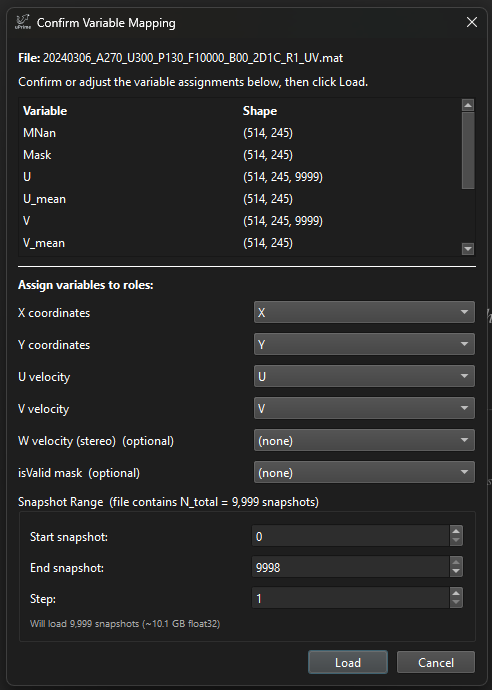
\includegraphics[width=0.65\linewidth]{fig_mat_dialog}
  \caption{\texttt{.mat} variable confirmation dialog. The top panel lists every variable in the file with its shape. Six dropdowns map the file variables to \software{uPrime}'s expected roles ($x$, $y$, $U$, $V$, $W$, isValid); auto-detected matches are pre-filled. The bottom panel sets the snapshot subset to load (start, end, step), with a live readout of the resulting count and estimated memory size. Click \uipth{Load} to confirm and start the actual data read.}
  \label{fig:matdialog}
\end{figure}

\paragraph{Snapshot subset.} The dialog includes Start, End, and Step spinboxes. They allow loading only a slice (e.g.\ snapshots 0--999) or a strided subsample (e.g.\ every 10th snapshot from 0 to 9999). The estimated in-memory size updates live. This is useful for preliminary inspection of very large files before committing to the full load.

\paragraph{Progress feedback.} For v7.3 files (HDF5), the read is chunked snapshot-by-snapshot and the progress bar advances determinately. For classic \texttt{.mat} files, the read is a single blocking call from \texttt{scipy.io}, so a busy indicator is shown along with the file size in the status bar. After the read, the status bar prints a confirmation listing the chosen variables and snapshot count, for example:

\begin{center}
\texttt{Loaded .mat: x=X, y=Y, u=U, v=V, w=(none), isValid=(none), N=1000 of 9999 (range 0:9990 step 10)}
\end{center}

\begin{tipbox}
For very large \texttt{.mat} files, save with \texttt{-v7.3} in MATLAB:\\
\texttt{save('dataset.mat', 'x', 'y', 'u', 'v', '-v7.3')}\\
This enables HDF5 chunked reading, which can show real per-snapshot progress and avoids loading the entire file in one blocking call.
\end{tipbox}

\begin{warnbox}
A \texttt{.mat} file containing a single snapshot will be rejected before any data is read (Figure~\ref{fig:singlesnap}). Most \software{uPrime} modules require multiple snapshots to compute statistics; for a single snapshot only the field viewer is meaningful, which does not justify loading the file.
\end{warnbox}

\begin{figure}[htbp]
  \centering
  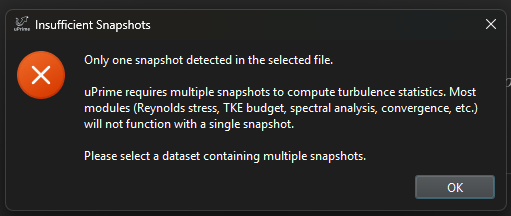
\includegraphics[width=0.55\linewidth]{fig_mat_singlesnap_error}
  \caption{Error dialog shown when a \texttt{.mat} file contains only one snapshot. The check is performed on the metadata before any data is loaded, so the error appears immediately regardless of the file size.}
  \label{fig:singlesnap}
\end{figure}

% ============================= CHAPTER 2 ==============================
\chapter{Main Window}
\label{ch:main}

\section{Overview}

When \software{uPrime} launches you will see a welcome screen. The sidebar on the left is your control panel. All steps are numbered in the order you should use them.

\begin{figure}[htbp]
  \centering
  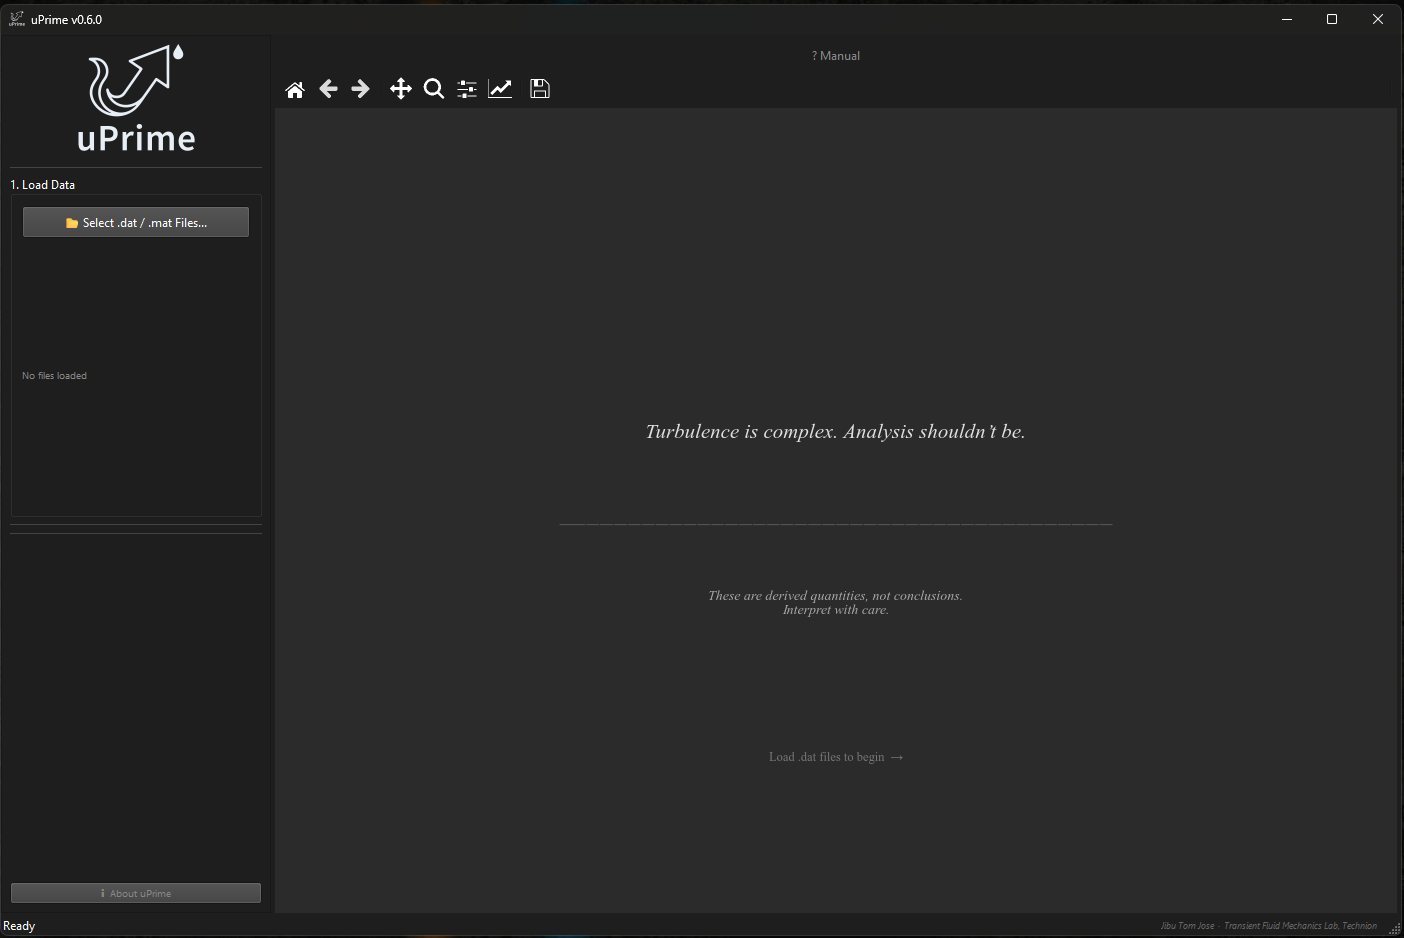
\includegraphics[width=0.92\linewidth]{fig0}
  \caption{\software{uPrime} v0.6.0 welcome screen on launch. The sidebar shows Step~1 (Load Data) only. The \uipth{? Manual} button is visible in the top right. Load \texttt{.dat} or \texttt{.mat} files from the sidebar to begin.}
  \label{fig:welcome}
\end{figure}

\begin{figure}[htbp]
  \centering
  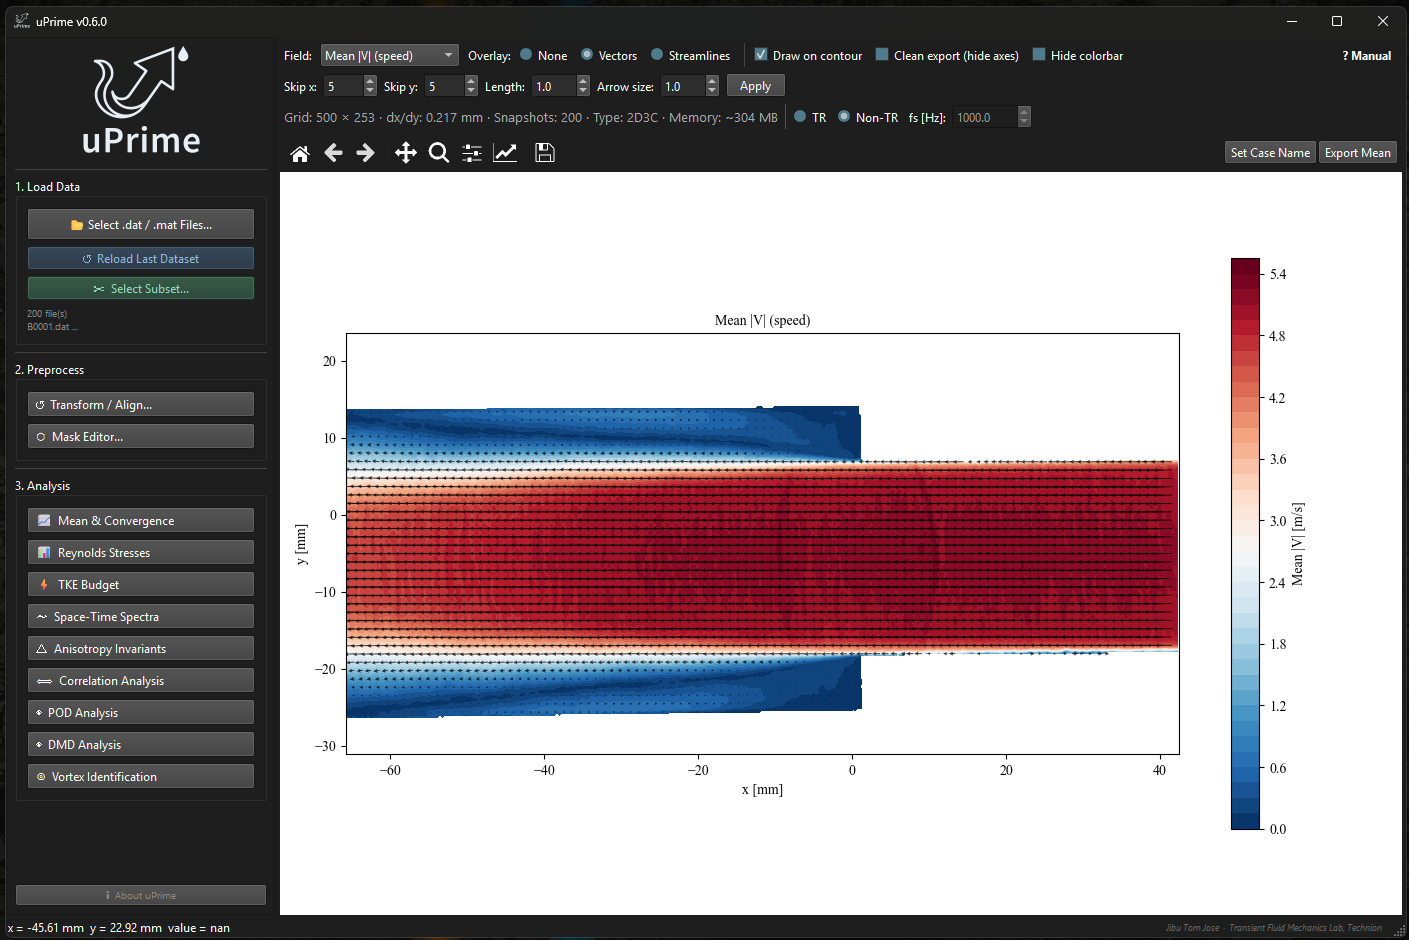
\includegraphics[width=0.85\linewidth]{fig1}
  \caption{Main window after loading a dataset. The Analysis panel lists modules in the recommended order of use, beginning with \uipth{Mean \& Convergence} for verifying statistical convergence before moving to higher-order statistics.}
  \label{fig:main}
\end{figure}

\subsection{Step 1: Load Data}

Click \uipth{Select .dat / .mat Files\ldots} to open a file browser. You can select multiple \texttt{.dat} files (one snapshot each) or a single \texttt{.mat} file (full time series). The file type is auto-detected from the extension.

For \texttt{.dat} loads, a subsampling dialog appears next (see Section~\ref{sec:subsample}). For \texttt{.mat} loads, the variable confirmation dialog appears (see Section~\ref{sec:matformat}).

After loading, the acquisition-type dialog appears. Set \uipth{TR} (time-resolved) or \uipth{Non-TR} and enter the sampling frequency $f_s$ if TR.

\begin{figure}[htbp]
  \centering
  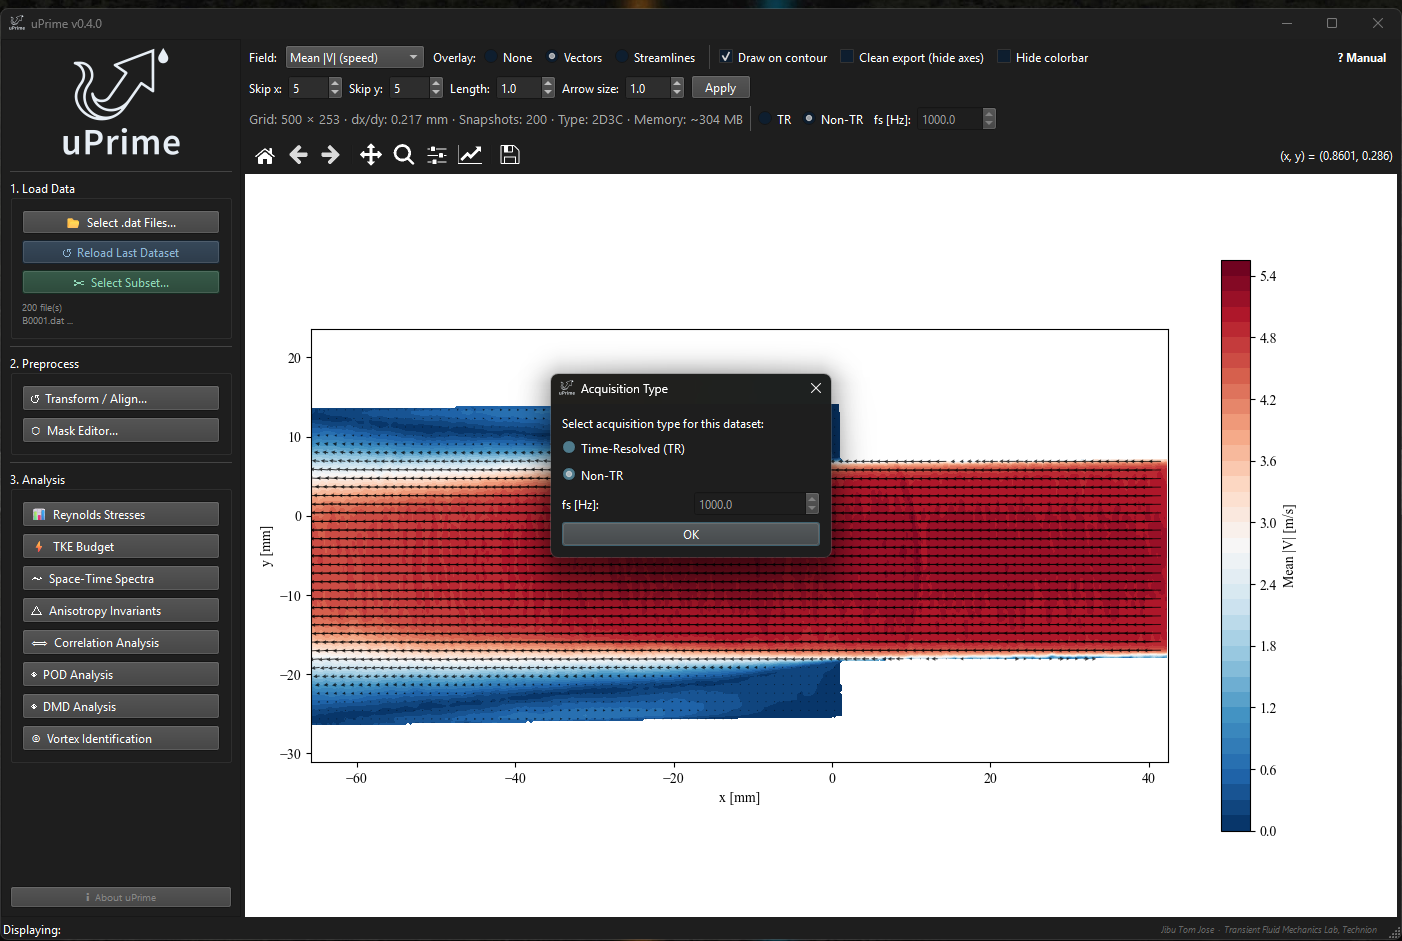
\includegraphics[width=0.85\linewidth]{fig_acqtype}
  \caption{Acquisition type dialog shown automatically after each data load. Select TR and enter $f_s$ to enable temporal analysis modules. The $f_s$ spinbox is greyed out when Non-TR is selected.}
  \label{fig:acqtype}
\end{figure}

\subsection{Step 2: Preprocess}

Click \uipth{Transform / Align\ldots} to open the coordinate correction tool. This is where you fix camera tilt, shift the coordinate origin, and optionally mirror the dataset. \textbf{Always do this before running any analysis.} Full details are in Chapter~\ref{ch:transform}.

Click \uipth{Mask Editor\ldots} to draw additional spatial masks over regions you want to exclude from analysis (e.g.\ reflections, shadows, or wall regions not detected by the DaVis isValid flag). Masks are non-destructive: the raw velocity data is never modified. Toggling a mask on or off does not require reloading.

\begin{figure}[htbp]
  \centering
  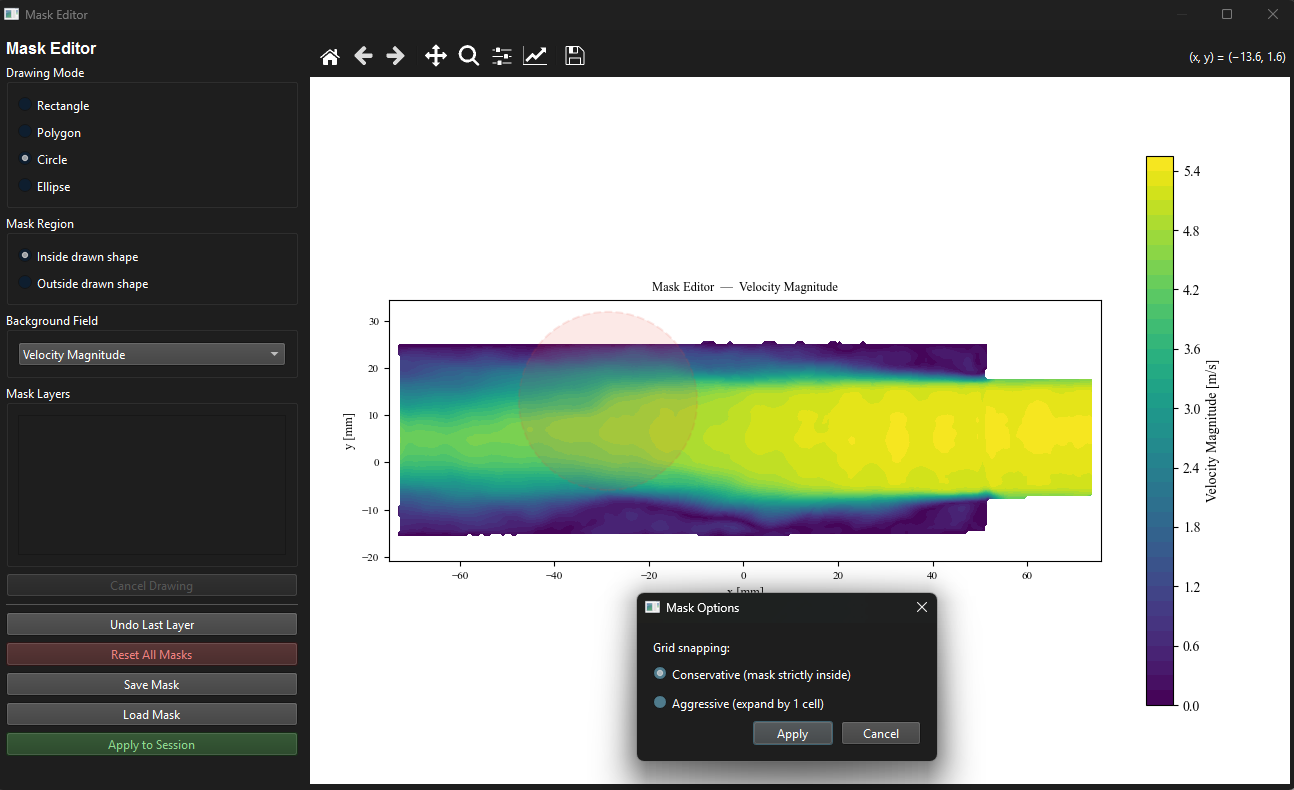
\includegraphics[width=0.92\linewidth]{fig_maskeditor}
  \caption{Mask Editor window. The user is drawing a polygon (red) over a region to exclude. Drawing modes include Rectangle, Polygon, Circle, and Ellipse. The mask can be applied inside or outside the drawn shape. Multiple layers can be stacked and each can be undone independently.}
  \label{fig:maskeditor}
\end{figure}

\begin{figure}[htbp]
  \centering
  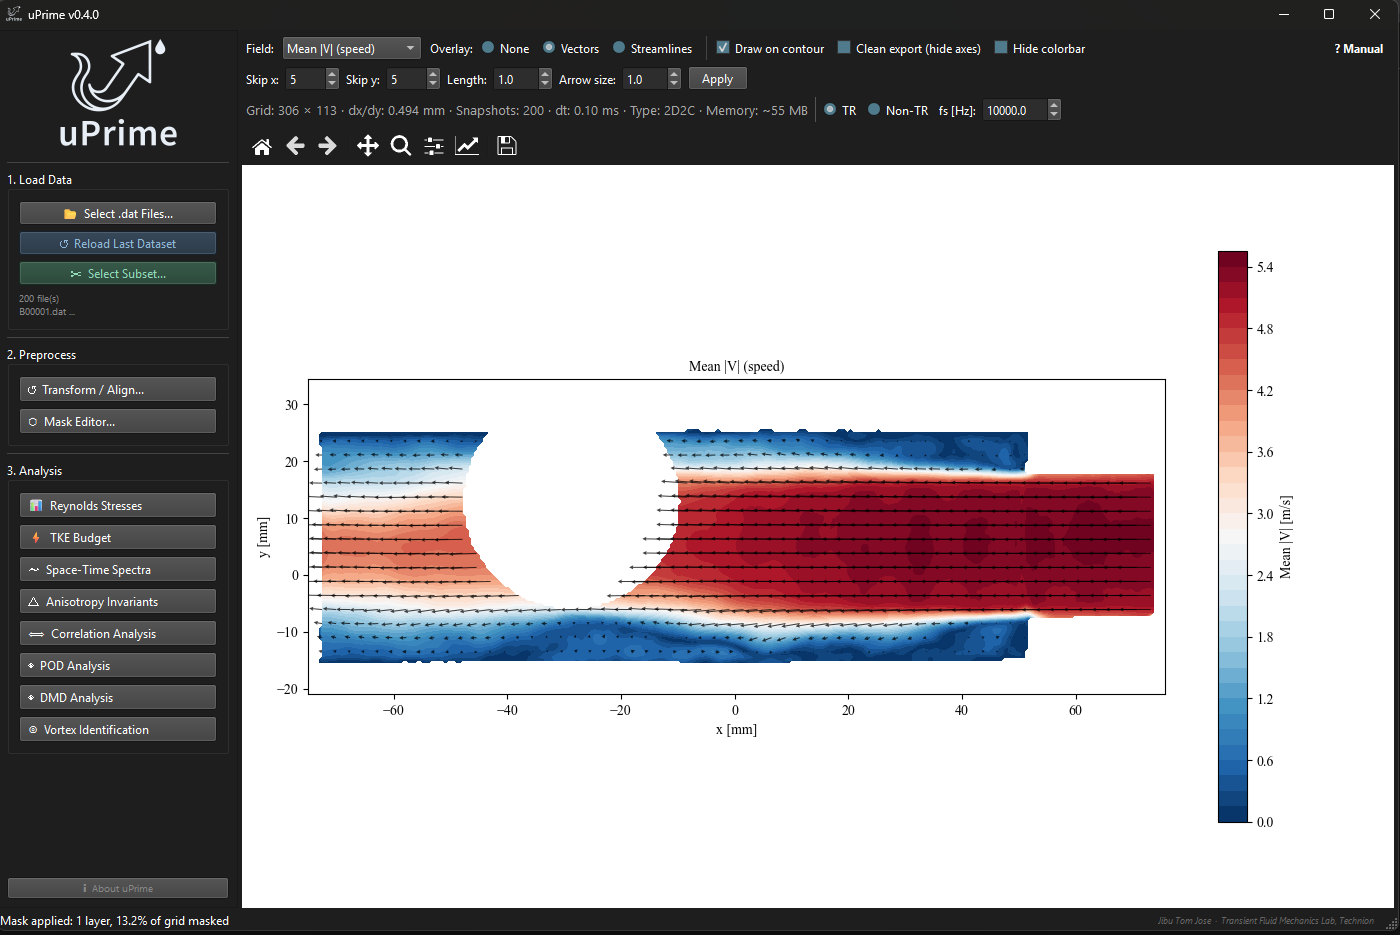
\includegraphics[width=0.92\linewidth]{fig_mask_main}
  \caption{Main window after applying a drawn mask. The masked region is shown in white. The status bar at the bottom reports the number of mask layers and the fraction of the grid that is masked.}
  \label{fig:maskmain}
\end{figure}

\subsection{Step 3: Analysis}

Click any analysis button to open that module in its own window. Multiple analysis windows can be open at the same time and can be compared side by side. The recommended starting point is \uipth{Mean \& Convergence} (Chapter~\ref{ch:meanconv}); from there proceed to Reynolds stresses, TKE budget, and the higher-order modules as appropriate.

All heavy computations (POD, DMD, TKE budget, correlation, vortex identification) run in a background thread so the main window remains fully responsive during computation. A progress indicator appears below the compute button while the calculation is in progress.

\section{Acquisition type and sampling frequency}

The acquisition type and sampling frequency $f_s$ are set in the dataset info ribbon at the top of the main window, immediately below the field options strip. A dialog to set these values also appears automatically after each data load.

\begin{itemize}[leftmargin=1.5em]
  \item \uipth{TR}: snapshots are acquired at a fixed rate. Enter $f_s$ in Hz (enabled only for TR). Temporal analyzes (temporal spectra, temporal correlation, POD temporal coefficients, DMD) become available.
  \item \uipth{Non-TR}: snapshots are statistically independent (e.g.\ double-frame PIV). Temporal analyzes are greyed out.
\end{itemize}

\begin{warnbox}
Set the correct acquisition type and $f_s$ before opening any analysis window. Analysis windows read these settings when they open.
\end{warnbox}

\section{Dataset info ribbon}
\label{sec:datasetinfo}

A compact info strip appears just below the options strip after loading:

\begin{center}
\texttt{Grid: 507\,$\times$\,248 $\cdot$ dx/dy: 0.165\,mm $\cdot$ Snapshots: 2000 $\cdot$ dt: 0.10\,ms $\cdot$ Type: 2D2C $\cdot$ Memory: \textasciitilde{}2012\,MB}
\end{center}

\begin{itemize}[leftmargin=1.5em]
  \item \textbf{Grid}: number of velocity vectors in $x$ and $y$.
  \item \textbf{dx / dy}: spatial resolution in mm. For \texttt{.mat} files this is estimated from the coordinate arrays using the median of differences (robust to small rounding at the edges). A non-uniform grid (more than 1\% variation in spacing) triggers a status-bar warning, since FFT and Welch spectra assume uniform grids.
  \item \textbf{Snapshots}: how many snapshots are currently active (reflects subsampling).
  \item \textbf{dt}: time between frames in milliseconds (TR data only; updates if $f_s$ or stride changes).
  \item \textbf{Type}: \texttt{2D2C} for planar PIV; \texttt{2D3C} for stereo PIV with $W$.
  \item \textbf{Memory}: estimated RAM used by the velocity arrays. For datasets exceeding 4\,GB, this reflects the size of the memory-mapped file on disk rather than physical RAM consumed (see Section~\ref{sec:subsample}).
\end{itemize}

\section{Field viewer}

The right panel shows the selected velocity field as a filled contour plot with optional velocity vectors.

\subsection{Display controls}

\begin{table}[htbp]
\centering
\caption{Field viewer display controls.}
\begin{tabular}{lp{9cm}}
\toprule
\textbf{Control} & \textbf{Description} \\
\midrule
Field         & Quantity to show: Mean U/V/W, speed $|V|$, vorticity, Std(U), Std(V) \\
Overlay       & None, Vectors, or Streamlines \\
Draw on contour & When checked, overlays the selected overlay on the filled contour \\
Clean export  & Hides all axis labels, tick marks, and the plot title for a clean exported image \\
Hide colorbar & Removes the colorbar from the plot \\
? Manual      & Opens the user manual PDF \\
\bottomrule
\end{tabular}
\end{table}

\subsection{Streamlines}

Streamlines trace the instantaneous mean velocity field and give a cleaner visual impression of the flow topology than arrow vectors, especially in regions with complex recirculation.

\begin{stepbox}
\begin{enumerate}[leftmargin=1.5em, topsep=2pt]
  \item Set \uipth{Overlay} to \uipth{Streamlines}.
  \item The vector ribbon appears. Left-click and drag on the field to draw a rake seed line. Multiple rakes can be drawn cumulatively.
  \item Adjust \uipth{Length}, color, and line width in the ribbon.
  \item Click \uipth{Apply} to redraw.
  \item Click \uipth{Reset} in the ribbon to clear all seed rakes and start over.
\end{enumerate}
\end{stepbox}

\begin{notebox}
Streamlines are drawn from the mean velocity field only. They do not reflect instantaneous snapshot structure.
\end{notebox}

\subsection{Toolbar}

\begin{table}[htbp]
\centering
\caption{Toolbar button functions.}
\begin{tabular}{ll}
\toprule
\textbf{Button} & \textbf{Function} \\
\midrule
Home           & Resets the view to the original limits, regardless of zoom history \\
Back / Forward & Step through zoom history \\
Pan            & Click and drag to pan the view \\
Zoom           & Click and drag a rectangle to zoom in \\
Save           & Save the figure as PNG (300 DPI), PDF, or SVG \\
\bottomrule
\end{tabular}
\end{table}

\subsection{Saving figures}

Click the Save button in the toolbar. PNG is saved at 300\,DPI. PDF and SVG use vector graphics; all text is saved as editable text and can be restyled in Adobe Illustrator or Inkscape.

\begin{tipbox}
For publication figures: (1) enable \uipth{Clean export} to hide axes, (2) enable \uipth{Hide colorbar} if not needed, (3) save as SVG and open in Illustrator to set your journal's font and size requirements.
\end{tipbox}

\section{Export menu}

The \uipth{Export} menu in the menu bar provides one-click export of the time-averaged mean field as a Tecplot ASCII \texttt{.dat} file. The exported file contains $\langle U \rangle$, $\langle V \rangle$, $|V|$, and (for stereo data) $\langle W \rangle$ on the original grid, ready for use in CFD validation, plotting in Tecplot, or import into other PIV tools.

\begin{figure}[htbp]
  \centering
  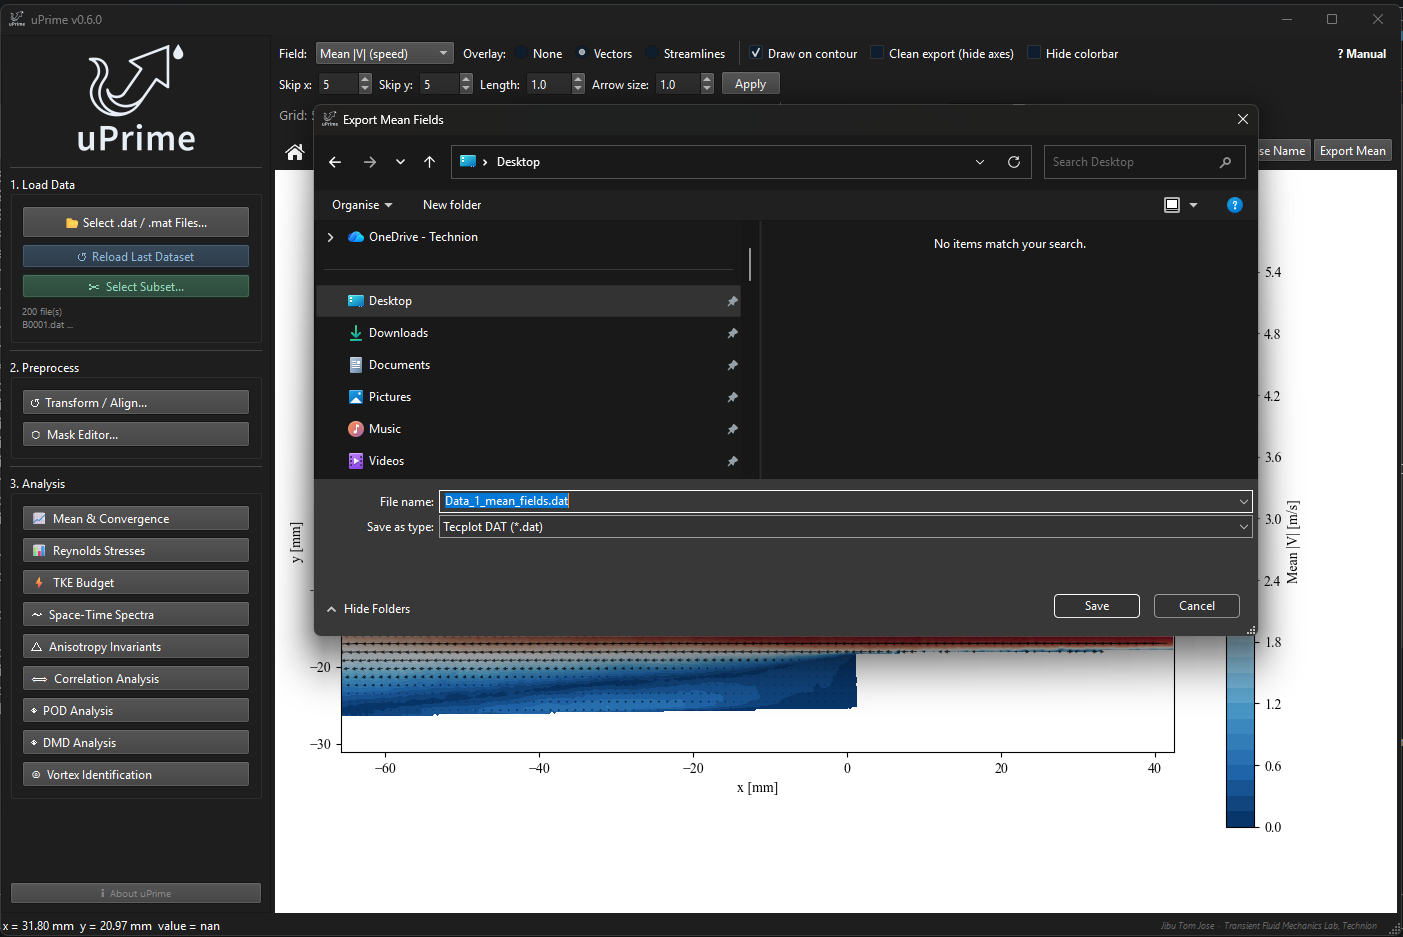
\includegraphics[width=0.6\linewidth]{fig_export_menu}
  \caption{Main window \uipth{Export} menu showing the Tecplot ASCII mean field export option.}
  \label{fig:exportmenu}
\end{figure}

\section{Snapshot subsampling and large dataset handling}
\label{sec:subsample}

A subsampling dialog appears whenever \texttt{.dat} files are selected, giving you control over how many snapshots to load. The same controls (start, end, step) are available inside the \texttt{.mat} variable confirmation dialog (Section~\ref{sec:matformat}).

\begin{itemize}[leftmargin=1.5em]
  \item \textbf{Load all}: load every file in the selection.
  \item \textbf{Stride}: load every $K$-th snapshot. Stride~5 on a 10,000-snapshot dataset gives 2000 samples, which is sufficient for mean fields, Reynolds stresses, and correlations.
  \item \textbf{Limit}: load only the first $N$ snapshots.
\end{itemize}

The dialog shows the estimated snapshot count and memory usage, updating live as you change the options.

After loading, click \uipth{Select Subset\ldots} to adjust the active snapshot range without re-reading from disk.

\begin{tipbox}
For 10,000+ snapshot datasets, start with Stride~5 ($\sim$2000 samples). Mean fields and Reynolds stresses converge well at this level. Run POD and DMD on the full set once you know what you are looking for. Use the \uipth{Mean \& Convergence} module (Chapter~\ref{ch:meanconv}) to verify whether your subsample is sufficient.
\end{tipbox}

\subsection{Large dataset handling (datasets exceeding 4\,GB)}

When the estimated dataset size after subsampling exceeds 4\,GB, \software{uPrime} automatically switches to a \textbf{memory-mapped} loading strategy. Instead of loading all velocity data into RAM, \software{uPrime} writes the data to a temporary binary file on your system's temp drive (typically \texttt{C:\textbackslash Users\textbackslash \textit{username}\textbackslash AppData\textbackslash Local\textbackslash Temp}) and accesses it as needed. The actual path is shown in the warning label inside the subsampling dialog.

\begin{notebox}
Memory-mapped loading requires free disk space on your system temp drive equal to the dataset size. For a 10,000-snapshot 2D2C dataset at a typical grid size, this is approximately 10\,GB. The temporary file is deleted automatically when \software{uPrime} closes normally.
\end{notebox}

\begin{warnbox}
If \software{uPrime} crashes or is forcibly closed, the temporary file may not be deleted. In that case, navigate to your system temp folder and delete any files named \texttt{uprime\_memmap\_*.bin} manually to recover disk space.
\end{warnbox}

The key practical differences when memory-mapped loading is active:

\begin{itemize}[leftmargin=1.5em]
  \item \textbf{Initial load is slower}: \software{uPrime} writes the full dataset to disk before opening it. On a fast SSD, expect 30--90 seconds for a 10\,GB dataset in addition to the normal file reading time.
  \item \textbf{All analysis works normally}: POD, DMD, TKE budget, spectra, correlation, and vortex identification all function identically. Memory-mapped arrays behave like regular numpy arrays.
  \item \textbf{RAM usage is reduced}: only the pages of data currently being accessed are held in RAM. The operating system manages this automatically.
  \item \textbf{Do not load from external drives}: if your \texttt{.dat} files are on an external HDD, copy them to a local drive first. Reading from an external drive while also writing the memory-mapped cache to the temp drive simultaneously will be very slow.
\end{itemize}

\begin{tipbox}
If your system temp drive (usually C:) does not have enough free space, use Stride subsampling to reduce the dataset to under 4\,GB before loading. For example, Stride~3 on a 10,000-snapshot dataset gives $\sim$3333 snapshots ($\sim$3.3\,GB for a typical 2D2C grid), which stays below the threshold and loads entirely into RAM.
\end{tipbox}

% ============================= CHAPTER 3 ==============================
\chapter{Coordinate Transform}
\label{ch:transform}

Open from \uipth{2.\ Preprocess $\to$ Transform / Align\ldots}.

\begin{warnbox}
Transforms modify the dataset \textbf{in memory} and cannot be undone. If you make a mistake, click \uipth{Reload Last Dataset} in the sidebar to reload from disk and start again.
\end{warnbox}

In PIV experiments, the camera is rarely perfectly aligned with the flow geometry. Even a $1^\circ$ tilt introduces errors in all derived quantities, including mean profiles, Reynolds stresses, line profiles, and integral scales. Always apply the transform \emph{before} opening any analysis module.

\begin{figure}[htbp]
  \centering
  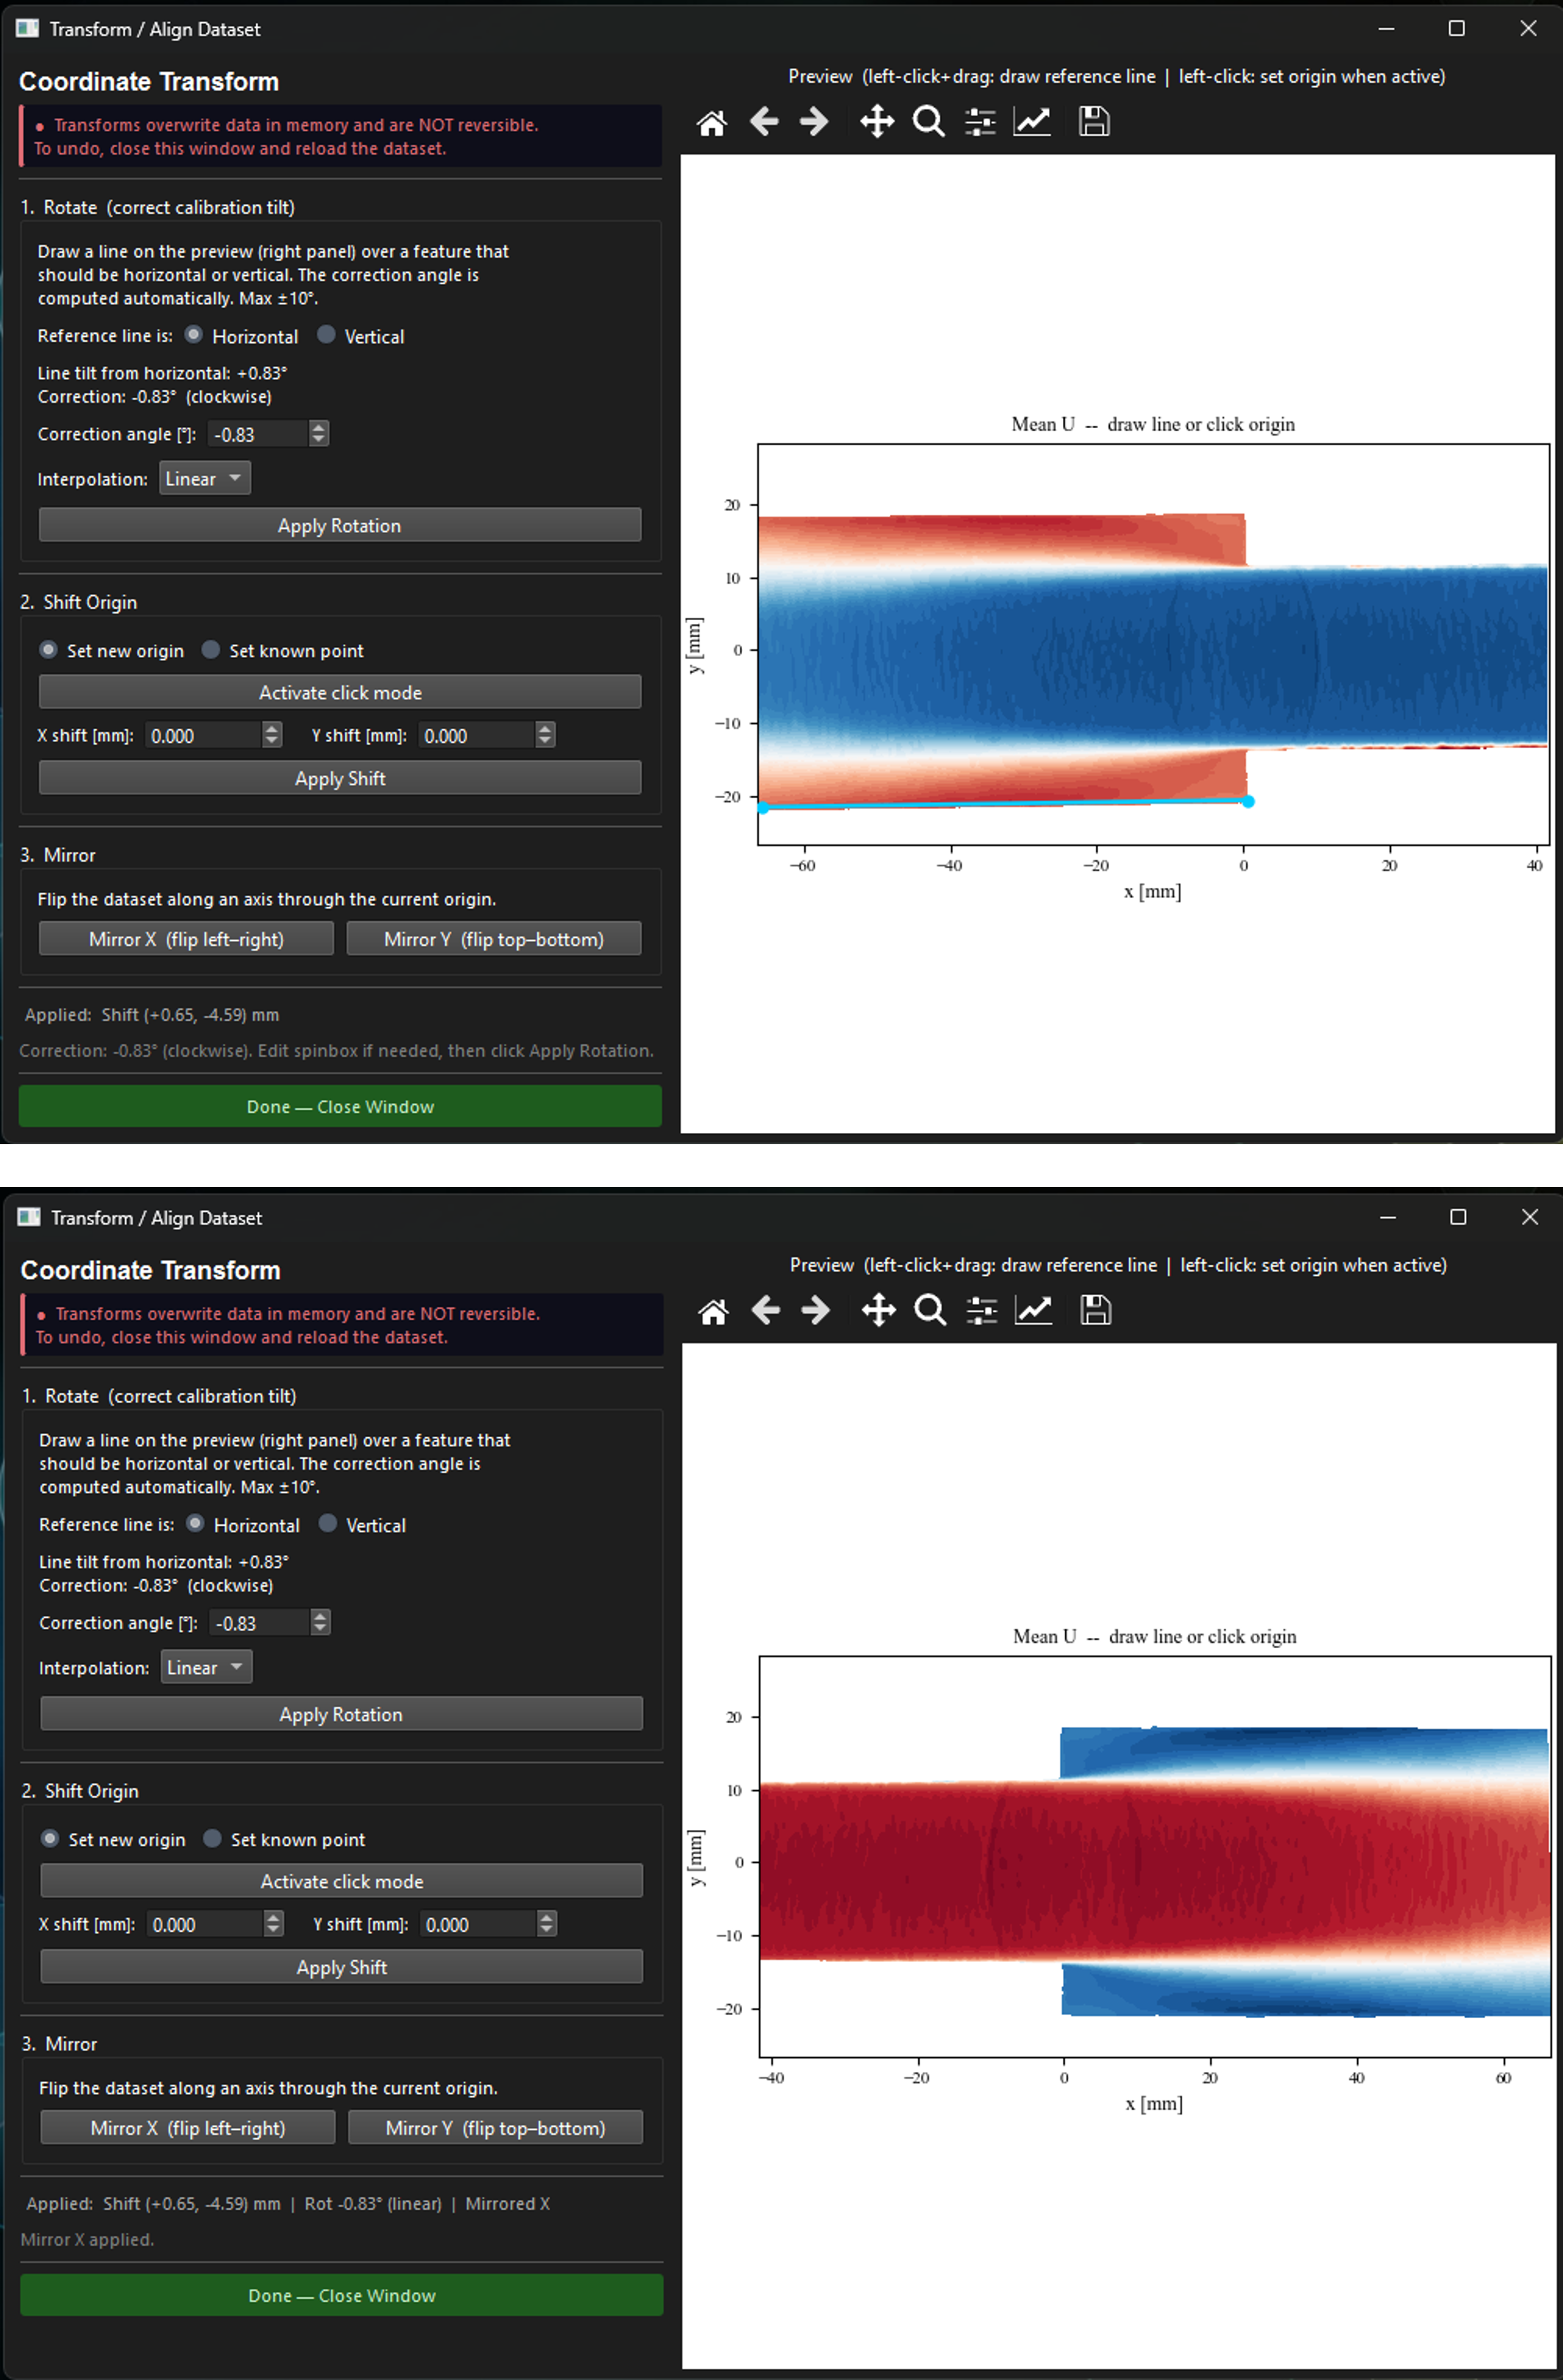
\includegraphics[width=0.92\linewidth]{fig11}
  \caption{Coordinate Transform window. Left: controls. Right: live preview of the mean field. A reference line drawn along the lower pipe wall is shown in cyan. The computed correction angle appears automatically in the left panel.}
  \label{fig:transform}
\end{figure}

\section{Rotation}

\begin{stepbox}
\begin{enumerate}[leftmargin=1.5em, topsep=2pt]
  \item Left-click and drag on the field preview to draw a reference line along any feature that should be perfectly horizontal or vertical (wall, step edge, pipe centerline).
  \item The misalignment angle is computed automatically and shown in the \uipth{Correction angle} field.
  \item Choose \uipth{Linear} (fast) or \uipth{Cubic} (smoother, recommended for final results).
  \item Click \uipth{Apply Rotation}.
\end{enumerate}
\end{stepbox}

\begin{notebox}
Rotation is limited to $\pm10^\circ$. For larger corrections, fix the calibration in DaVis and re-export your data.
\end{notebox}

\section{Origin shift}

Moves the coordinate origin $(0, 0)$ to a physically meaningful reference point such as a step corner, pipe inlet, or cylinder center. Two modes are available: \uipth{Set new origin} (click on the point that should become $(0, 0)$) and \uipth{Set known point} (click a point and enter what its real-world coordinates should be).

\section{Mirror}

Flips the entire dataset along an axis through the current origin. \uipth{Mirror X} negates all $x$-coordinates and the $U$ component; \uipth{Mirror Y} negates all $y$-coordinates and the $V$ component.

% ============================= CHAPTER 4 ==============================
\chapter{Mean \& Convergence}
\label{ch:meanconv}

Open from \uipth{3.\ Analysis $\to$ Mean \& Convergence}.

The Mean \& Convergence module is the recommended first stop for any new dataset. It serves two purposes: plotting mean velocity profiles along arbitrary lines (similar to the Reynolds stress line-profile mode but for first-order statistics), and quantitatively verifying that the dataset has enough snapshots for the higher-order statistics computed by other modules to be trustworthy.

The module has two tabs: \uipth{Mean Velocity} (line profiles) and \uipth{Convergence} (cumulative statistics at a picked point).

\section{Mean Velocity tab}
\label{sec:meanvel}

This tab plots $\langle U \rangle$, $\langle V \rangle$, and (for stereo data) $\langle W \rangle$ along a user-drawn line, in the same style as Reynolds stress line profiles.

\begin{stepbox}
\begin{enumerate}[leftmargin=1.5em, topsep=2pt]
  \item Choose line orientation: \uipth{Free}, \uipth{Horizontal}, or \uipth{Vertical}.
  \item For Horizontal or Vertical, set \uipth{Spatial avg $\pm$ pts} to average over neighboring rows or columns and reduce noise.
  \item Left-click and drag on the |⟨U⟩| field (left panel) to draw the line.
  \item Click \uipth{Plot Profile}.
\end{enumerate}
\end{stepbox}

\begin{figure}[htbp]
  \centering
  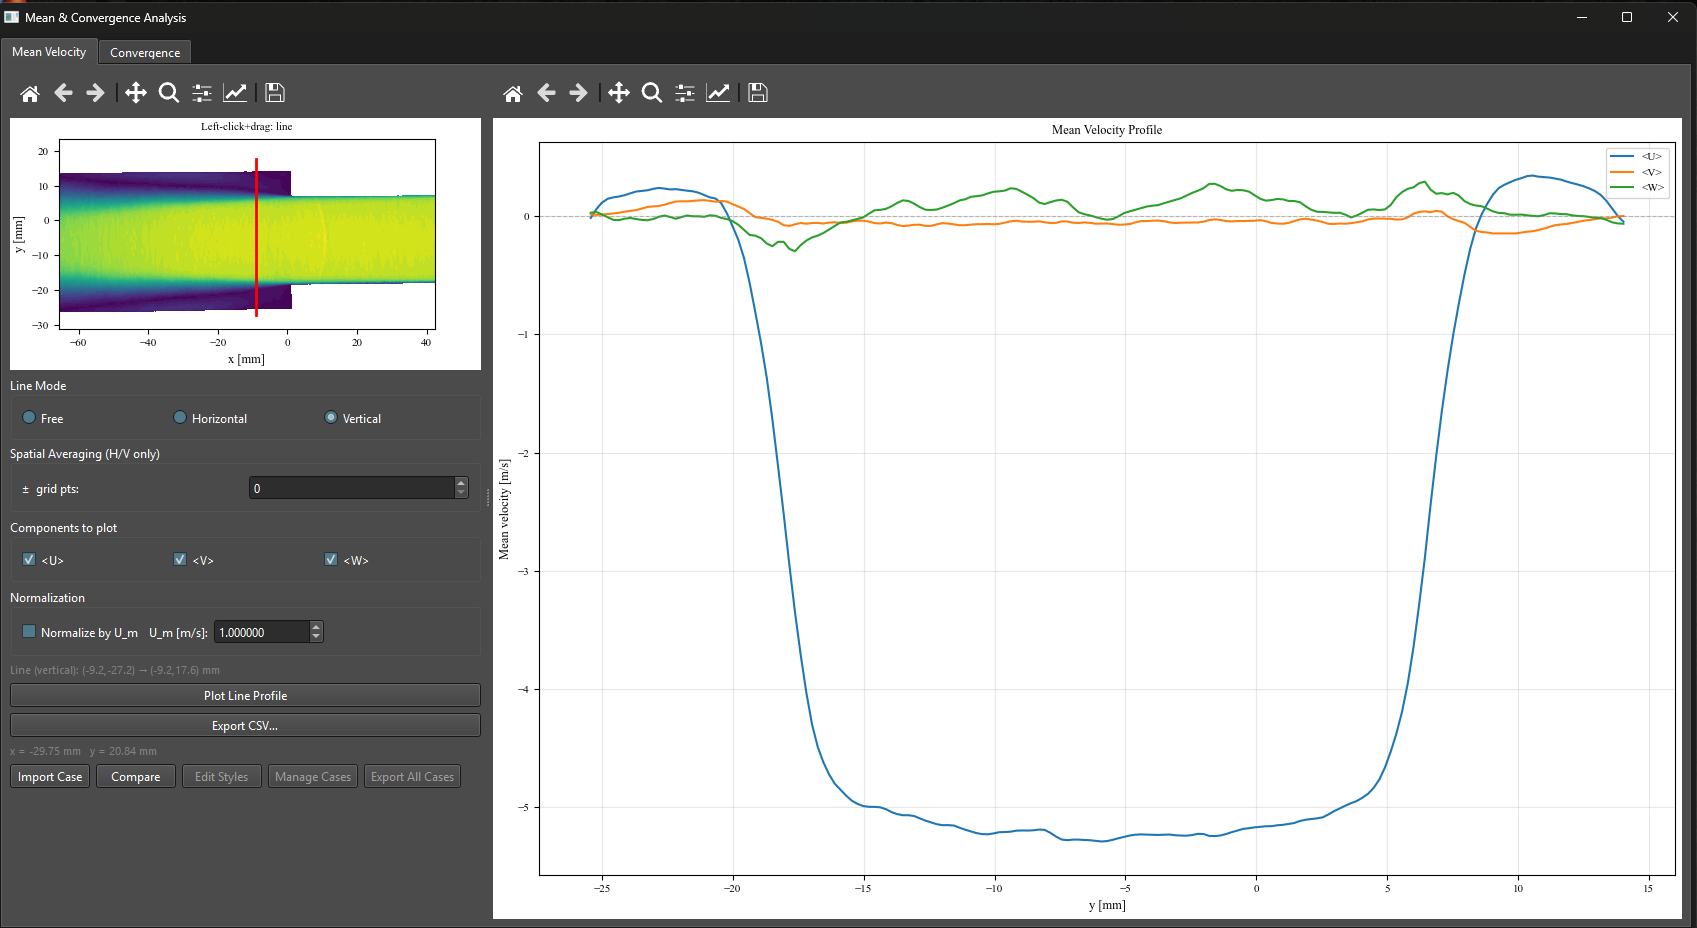
\includegraphics[width=0.92\linewidth]{fig_meanconv_meanvel}
  \caption{Mean \& Convergence module, Mean Velocity tab. Left: $|\langle U \rangle|$ field with a free line drawn (cyan). Right: $\langle U \rangle$, $\langle V \rangle$ profiles along the line as a function of arc length. Stereo data adds $\langle W \rangle$.}
  \label{fig:meanvel}
\end{figure}

\subsection{Normalization by $U_m$}

A checkbox labeled \uipth{Normalize by $U_m$} and a paired spinbox let you divide the plotted velocity components by a user-supplied bulk or reference velocity. When checked, the y-axis labels switch to \texttt{U/U\_m [-]}, \texttt{V/U\_m [-]}, etc. The arc-length axis is not normalized, matching the convention used elsewhere in \software{uPrime}.

\begin{tipbox}
Set $U_m$ to the bulk velocity, free-stream velocity, or any reference value for your flow. Profiles are then directly comparable across cases at different Reynolds numbers.
\end{tipbox}

\subsection{Multi-case comparison}
\label{sec:meanvel_compare}

\software{uPrime} can overlay imported cases (CSV files exported from previous \software{uPrime} sessions or other tools that follow the same column layout) on top of the current profile. This is useful for comparing experimental runs, conditions, or numerical-versus-experimental data.

\begin{stepbox}
\begin{enumerate}[leftmargin=1.5em, topsep=2pt]
  \item Click \uipth{Import Case\ldots} and select a CSV file.
  \item The imported case is added to the case list with an auto-assigned color and dashed linestyle.
  \item Use \uipth{Edit Styles\ldots} to change line color, style, marker, and label per case.
  \item Use \uipth{Manage Cases\ldots} to rename or remove cases.
  \item The current $U_m$ setting is compared against the \texttt{\# U\_m =} header in each imported CSV. If they differ, a status-bar warning is shown for that specific case so you can manually re-normalize before publishing.
\end{enumerate}
\end{stepbox}

The same multi-case workflow is available in Reynolds Stress, TKE Budget, Spectra, Correlation, and Anisotropy windows (see Chapter~\ref{ch:multicase}).

\subsection{Exporting}

Click \uipth{Export Profile\ldots} to save the current profile as a CSV file. The header records the line geometry (endpoints), the $U_m$ value (or N/A if normalization is off), and the column layout. Multi-case overlays can be exported together using \uipth{Export All Cases\ldots}.

\section{Convergence tab}
\label{sec:convergence}

The Convergence tab quantifies whether the dataset has enough snapshots for the first three moments of the velocity fluctuations to be statistically converged. This serves as a numerical check on the assumptions made by every other turbulence-statistics module.

\subsection{Background}

Given a sequence of $N$ snapshots, the cumulative running statistics are
\begin{align}
\langle u' \rangle_N      &= \frac{1}{N} \sum_{i=1}^{N} (u_i - \langle u \rangle_{\mathrm{final}}), \\
\langle u' u' \rangle_N   &= \frac{1}{N} \sum_{i=1}^{N} (u_i - \langle u \rangle_{\mathrm{final}})^2, \\
\langle u' u' u' \rangle_N &= \frac{1}{N} \sum_{i=1}^{N} (u_i - \langle u \rangle_{\mathrm{final}})^3,
\end{align}
where $\langle u \rangle_{\mathrm{final}}$ is the mean computed over all loaded snapshots. With this definition, the curves approach a non-zero asymptote as $N$ grows, which is what allows convergence to be visually inspected.

The cumulative moments are computed using Welford's online algorithm extended to the third central moment. This is a single-pass $O(N)$ computation, numerically stable, and avoids storing per-snapshot residuals.

A trailing-window stability criterion is used to find the convergence point $N^*$:
\[
N^* = \min\left\{ N \;:\; \frac{\max_{n \in [N - W, N]} q_n - \min_{n \in [N - W, N]} q_n}{\sigma_{\mathrm{scale}}} < \varepsilon \right\}
\]
where $W = \max(50, N/10)$ and $\sigma_{\mathrm{scale}}$ is component-aware: $\sqrt{\langle u'u'\rangle_{\mathrm{final}}}$ for first moments, $\langle u'u'\rangle_{\mathrm{final}}$ for second, and $\langle u'u'\rangle_{\mathrm{final}}^{3/2}$ for third (and similarly per-component for $v$ and $w$). The criterion further requires the inequality to hold continuously across the next $W$ samples (sustained crossing), which prevents spurious early matches when the trailing-window range happens to be small by chance.

\noindent\textbf{Reference:} Welford, B.P. (1962). Note on a method for calculating corrected sums of squares and products. \textit{Technometrics}, 4(3), 419--420.

\subsection{Using the tab}

\begin{stepbox}
\begin{enumerate}[leftmargin=1.5em, topsep=2pt]
  \item Set \uipth{Kernel size} (odd integer, default 3). The picked point is averaged over a $k \times k$ neighborhood. Larger kernels reduce noise but cannot pick points within $\lfloor k/2 \rfloor$ of the boundary.
  \item Left-click on the field to pick a point. Points within the boundary margin (shaded grey) are rejected with a status-bar message.
  \item Set the three thresholds: $\varepsilon_1$ for $\langle u' \rangle$, $\varepsilon_2$ for $\langle u'u' \rangle$, $\varepsilon_3$ for $\langle u'u'u' \rangle$. Default 1e-3 each.
  \item Tick which moment orders to plot: $\langle u' \rangle$, $\langle u'u' \rangle$, $\langle u'u'u' \rangle$.
  \item Choose \uipth{Grid layout} (one subplot per component-order combination, raw values) or \uipth{Single plot} (all selected curves overlaid, normalized).
  \item Click \uipth{Compute Convergence}.
\end{enumerate}
\end{stepbox}

\begin{figure}[htbp]
  \centering
  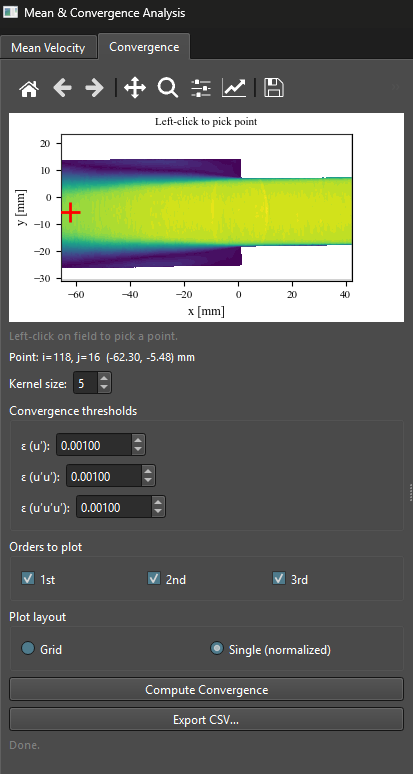
\includegraphics[width=0.6\linewidth]{fig_meanconv_picker}
  \caption{Convergence tab, point picker. The $|\langle U \rangle|$ field is shown in viridis. The boundary margin (grey overlay) is determined by the kernel size and clicks inside it are rejected. The picked point and kernel footprint are shown as a red marker.}
  \label{fig:convpicker}
\end{figure}

\subsection{Grid layout (raw values)}

In grid mode, $\langle u' \rangle_N$, $\langle u'u' \rangle_N$, and $\langle u'u'u' \rangle_N$ are plotted in physical units, one subplot per component (rows: $u$, $v$, optionally $w$) and per moment order (columns: 1, 2, 3). A pair of dashed horizontal lines marks the threshold band $q_{\mathrm{final}} \pm \varepsilon \cdot \sigma_{\mathrm{scale}}$ around the asymptote, and a vertical line at $N^*$ shows the sustained-crossing convergence point. Curves that never satisfy the criterion are labeled \uipth{Not converged}.

\begin{figure}[htbp]
  \centering
  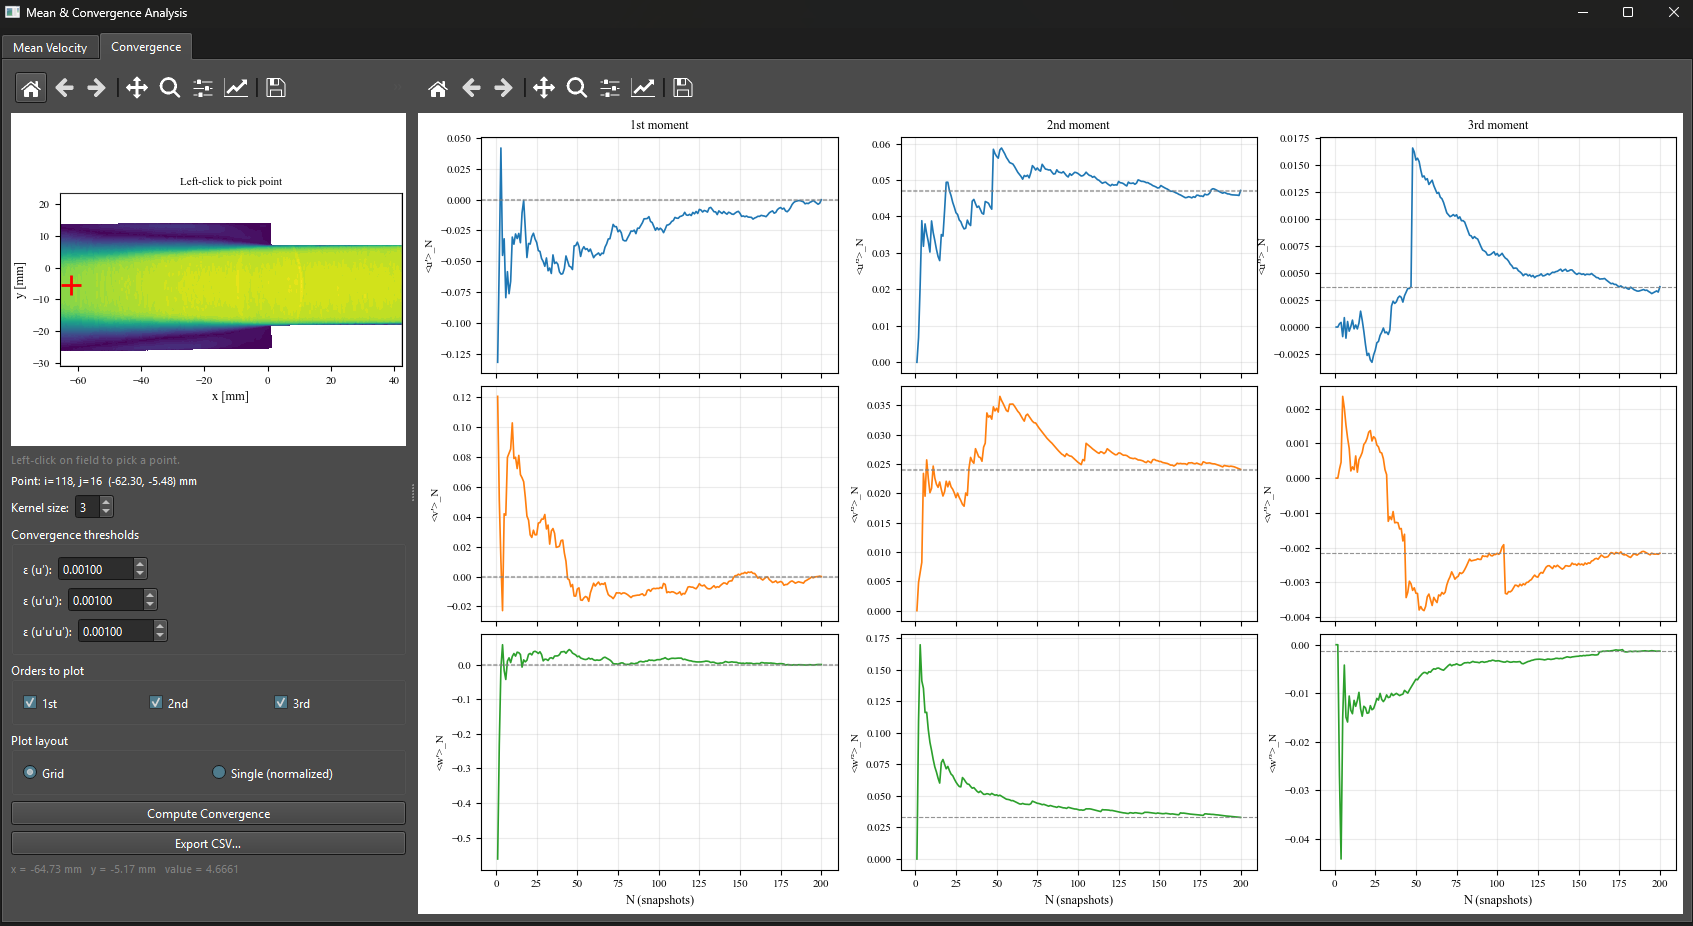
\includegraphics[width=0.92\linewidth]{fig_meanconv_grid}
  \caption{Convergence tab, grid layout (planar 2D2C: $2 \times 3$ subplots). Each panel shows a cumulative moment in physical units, the dashed threshold band around its final-value asymptote, and the vertical $N^*$ line where the sustained-crossing criterion is first met. Third moments typically require many more snapshots than first or second moments to converge.}
  \label{fig:convgrid}
\end{figure}

\subsection{Single plot (normalized)}

In single-plot mode, every selected curve is normalized by its own scale $\sigma_{\mathrm{scale}}$ so they share a common dimensionless y-axis. Curves are color-coded by component ($u$, $v$, $w$) and styled by moment order (solid for first, dashed for second, dotted for third). Per-component dashed threshold bands are drawn around each curve's asymptote $q_{\mathrm{final}}/\sigma_{\mathrm{scale}}$.

\begin{figure}[htbp]
  \centering
  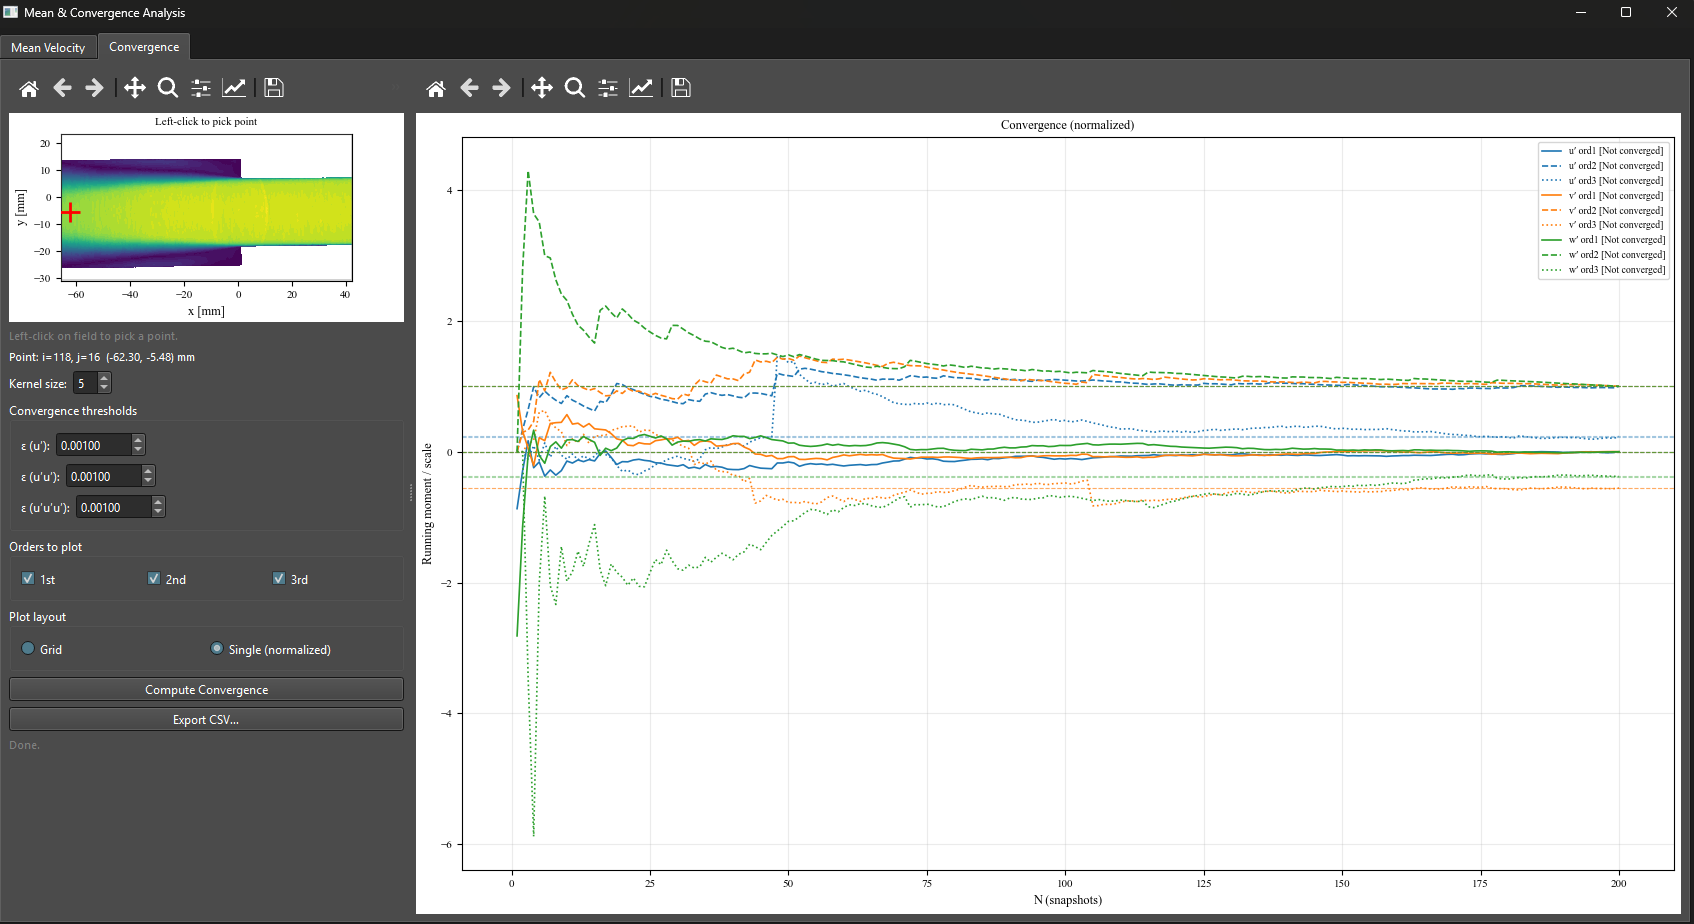
\includegraphics[width=0.92\linewidth]{fig_meanconv_single}
  \caption{Convergence tab, single normalized layout. All selected curves are overlaid on one axes and approach their respective non-zero asymptotes (one per curve). Per-component dashed threshold bands flank each asymptote.}
  \label{fig:convsingle}
\end{figure}

\subsection{Exporting}

Click \uipth{Export CSV\ldots} to save the cumulative moments. The header block records the picked point indices and physical coordinates, the kernel size, the three thresholds, the dataset $N_{\mathrm{total}}$, and the $N^*$ value computed for each quantity. The columns are $N$, $\langle u' \rangle_N$, $\langle u'u' \rangle_N$, $\langle u'u'u' \rangle_N$, $\langle v' \rangle_N$, ..., adding $w$ components for stereo data.

\begin{tipbox}
First and second moments typically converge with a few hundred snapshots in well-mixed regions. Third moments often require 5000 or more, and may not converge at all in regions of low intensity. A non-converging $\langle u'u'u' \rangle$ is not necessarily a problem for second-order statistics; the convergence module simply makes this explicit.
\end{tipbox}

\section{Inline non-convergence notice}
\label{sec:convnotice}

The Reynolds Stress, TKE Budget, and Spectral Analysis windows display a persistent amber top-bar label when the loaded dataset has fewer than 500 snapshots:

\begin{center}
\fcolorbox{upaccent!60}{red!5}{\parbox{0.85\linewidth}{\centering \small \faExclamationTriangle\quad Only \textbf{N=234} snapshots loaded. Statistics may not be converged. Use the Mean \& Convergence module to verify.}}
\end{center}

The label is hidden automatically when the dataset has 500 or more snapshots. Other modules (Correlation, Anisotropy, POD, DMD, Vortex Identification) are silent. The 500 threshold is hardcoded in \texttt{core/constants.py} as \texttt{CONVERGENCE\_WARNING\_N} and can be changed in source builds.

\begin{figure}[htbp]
  \centering
  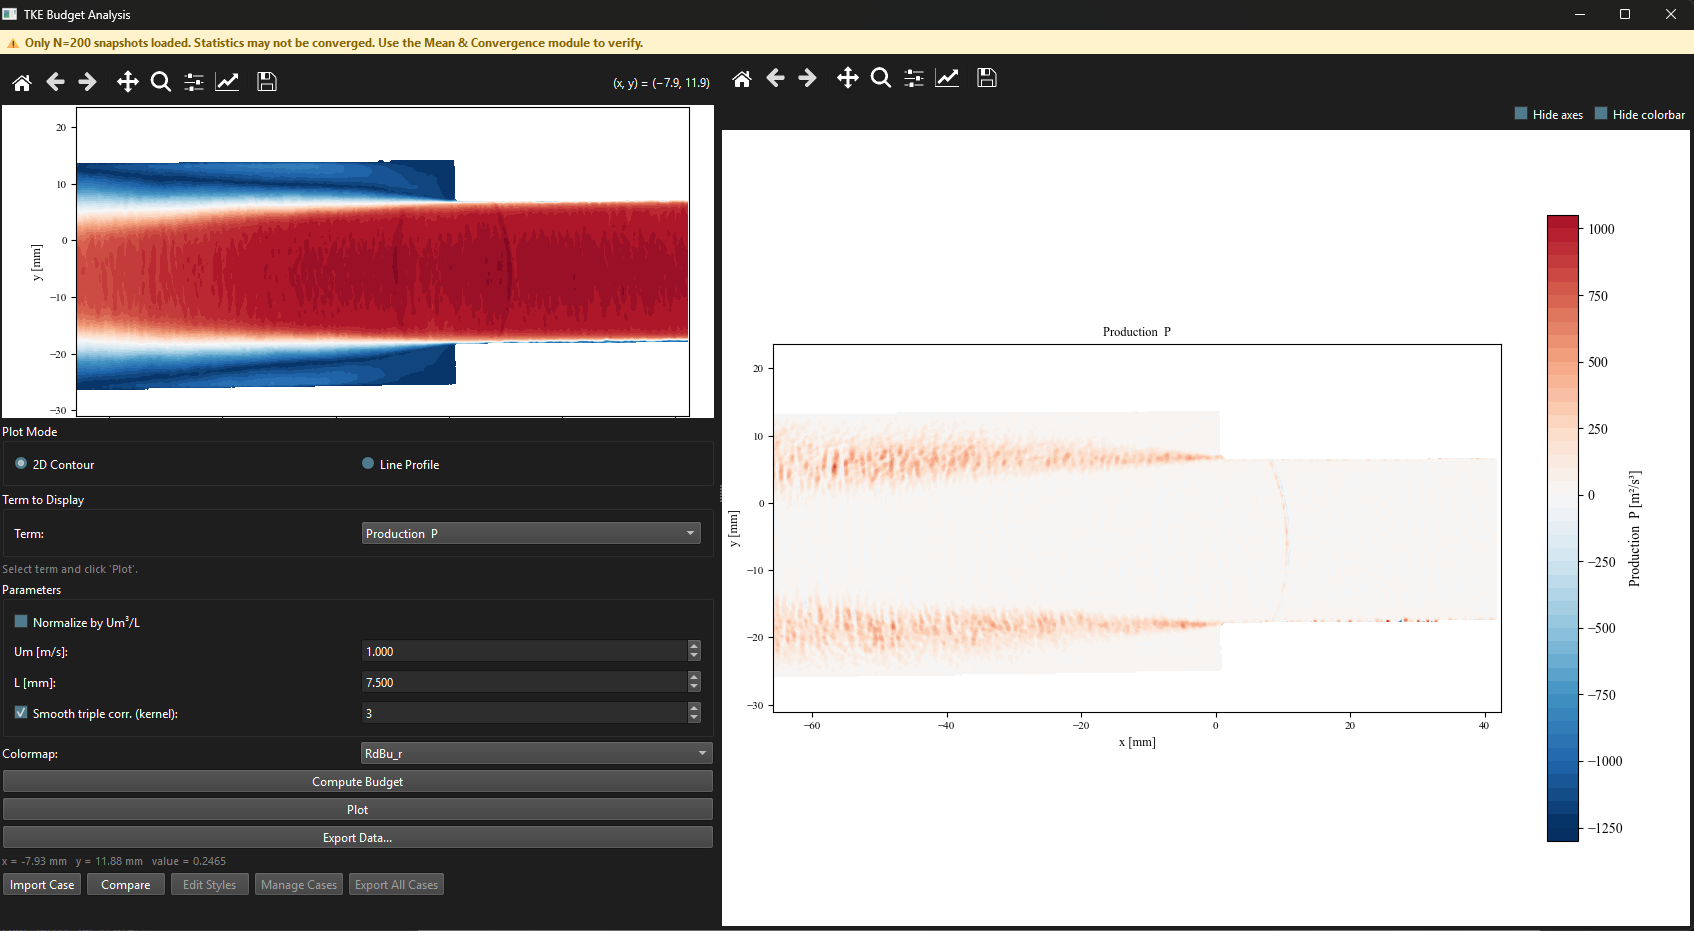
\includegraphics[width=0.85\linewidth]{fig_convergence_topbar}
  \caption{Top-bar non-convergence label as it appears in the Reynolds Stress window with $N = 234$ snapshots. The label is hidden automatically once $N \geq 500$.}
  \label{fig:convbar}
\end{figure}

% ============================= CHAPTER 5 ==============================
\chapter{Reynolds Stress Analysis}
\label{ch:reynolds}

Open from \uipth{3.\ Analysis $\to$ Reynolds Stresses}.

In turbulent flows, the instantaneous velocity can be decomposed into a time-averaged mean $\langle U_i \rangle$ and a fluctuating component $u'_i$, such that $U_i = \langle U_i \rangle + u'_i$. The Reynolds stress tensor $\langle u'_i u'_j \rangle$ quantifies the statistical intensity and directionality of these fluctuations and appears as a closure term in the Reynolds-Averaged Navier-Stokes (RANS) equations (Pope, 2000):
\[
\rho \frac{D \langle U_i \rangle}{Dt} = -\frac{\partial \langle p \rangle}{\partial x_i} + \mu \nabla^2 \langle U_i \rangle - \rho \frac{\partial \langle u'_i u'_j \rangle}{\partial x_j}
\]
The diagonal components $\langle u'u' \rangle$, $\langle v'v' \rangle$, $\langle w'w' \rangle$ are the normal stresses, directly related to the turbulent kinetic energy by $k = \tfrac{1}{2}(\langle u'u'\rangle + \langle v'v'\rangle + \langle w'w'\rangle)$. The off-diagonal components $\langle u'v' \rangle$, $\langle u'w' \rangle$, $\langle v'w' \rangle$ are the shear stresses, which are responsible for the turbulent momentum transfer across shear layers and boundary layers.

For 2D2C data, only $\langle u'u' \rangle$, $\langle v'v' \rangle$, and $\langle u'v' \rangle$ are available. All six components are computed for stereo (2D3C) data.

\begin{tipbox}
The shear stress $\langle u'v' \rangle$ is particularly useful for identifying shear layers and recirculation zones: it changes sign across the centreline of a jet or shear layer, and its peak magnitude locates the region of maximum turbulent momentum transfer.
\end{tipbox}

\noindent\textbf{Reference:} Pope, S.B. (2000). \textit{Turbulent Flows}. Cambridge University Press.

\section{2D contour map}

\begin{stepbox}
\begin{enumerate}[leftmargin=1.5em, topsep=2pt]
  \item Select \uipth{2D Contour Map} under Plot Mode.
  \item Choose the component from the \uipth{Component} dropdown.
  \item Optionally check \uipth{Scale by $U_m^2$} and enter the bulk velocity $U_m$ to non-dimensionalise.
  \item Click \uipth{Plot Contour}.
\end{enumerate}
\end{stepbox}

\begin{figure}[htbp]
  \centering
  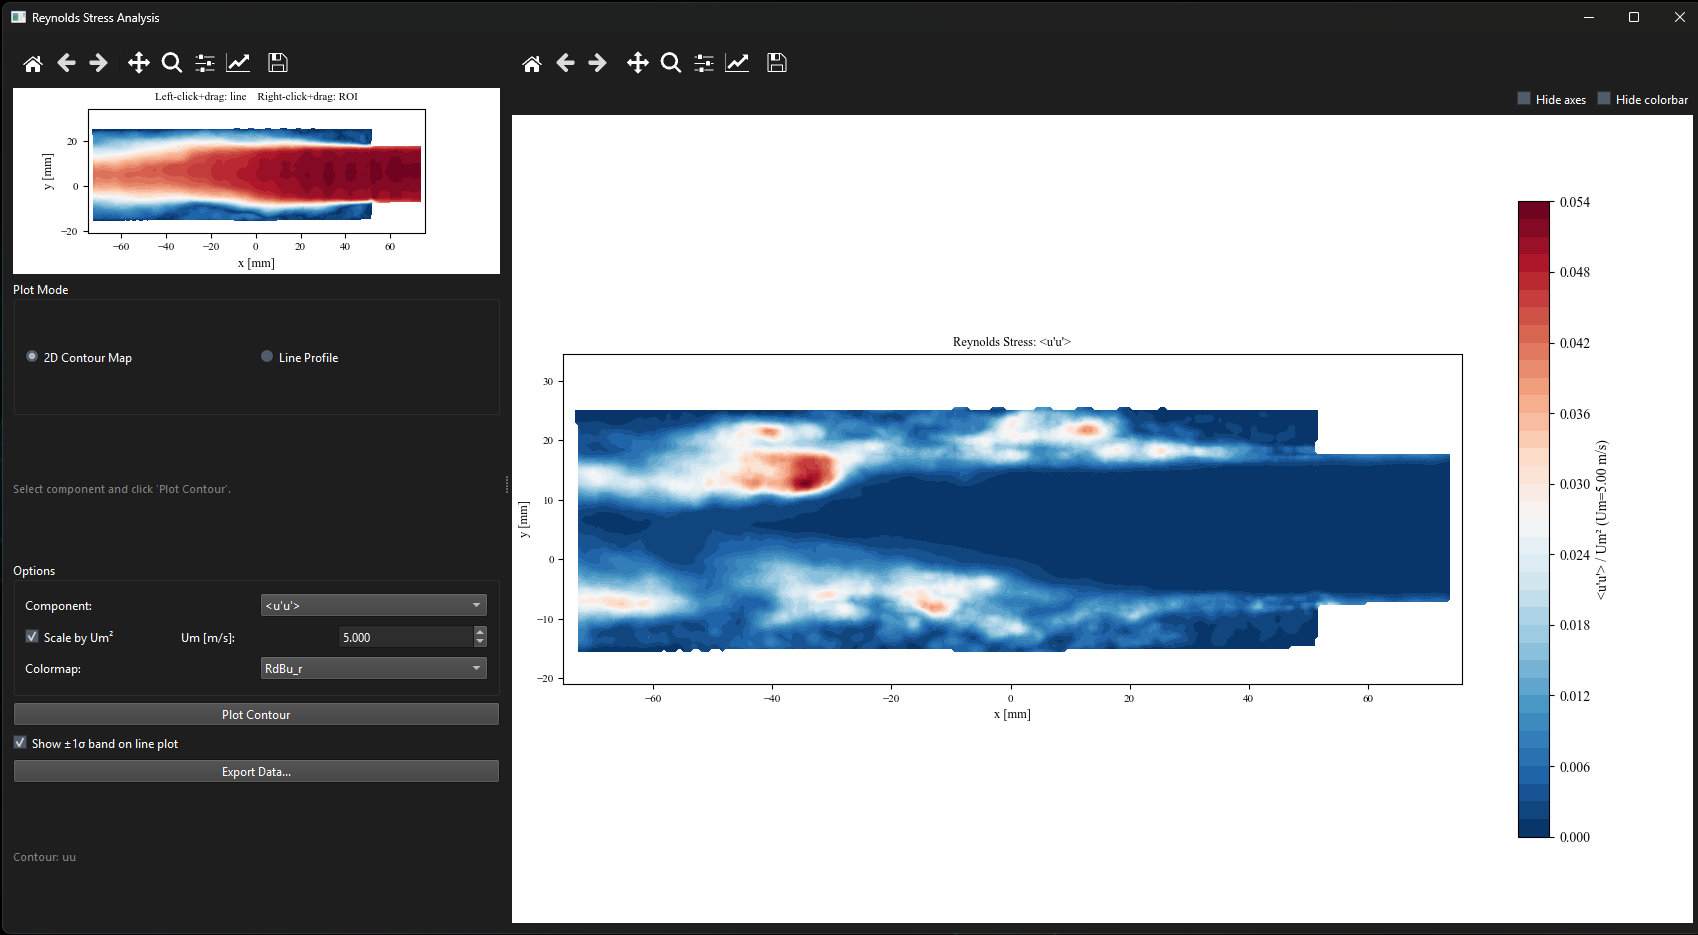
\includegraphics[width=0.92\linewidth]{fig2}
  \caption{Reynolds stress window in 2D contour mode showing $\langle u'v' \rangle$. The mean field is shown in the small reference panel on the left.}
  \label{fig:reynolds_contour}
\end{figure}

\section{Line profile}

\begin{stepbox}
\begin{enumerate}[leftmargin=1.5em, topsep=2pt]
  \item Select \uipth{Line Profile} under Plot Mode.
  \item Choose line orientation: \uipth{Free}, \uipth{Horizontal}, or \uipth{Vertical}.
  \item For Horizontal/Vertical, set \uipth{Spatial avg $\pm$ pts} to average over neighboring rows or columns and reduce noise.
  \item Left-click and drag on the left field panel to draw the line.
  \item Click \uipth{Plot Line Profile}.
\end{enumerate}
\end{stepbox}

All available stress components are plotted together. Check \uipth{Show $\pm1\sigma$ band} to display uncertainty bands. From v0.5.0 onward this checkbox is unchecked by default; the bands tend to crowd plots when multiple cases are overlaid for comparison.

\begin{figure}[htbp]
  \centering
  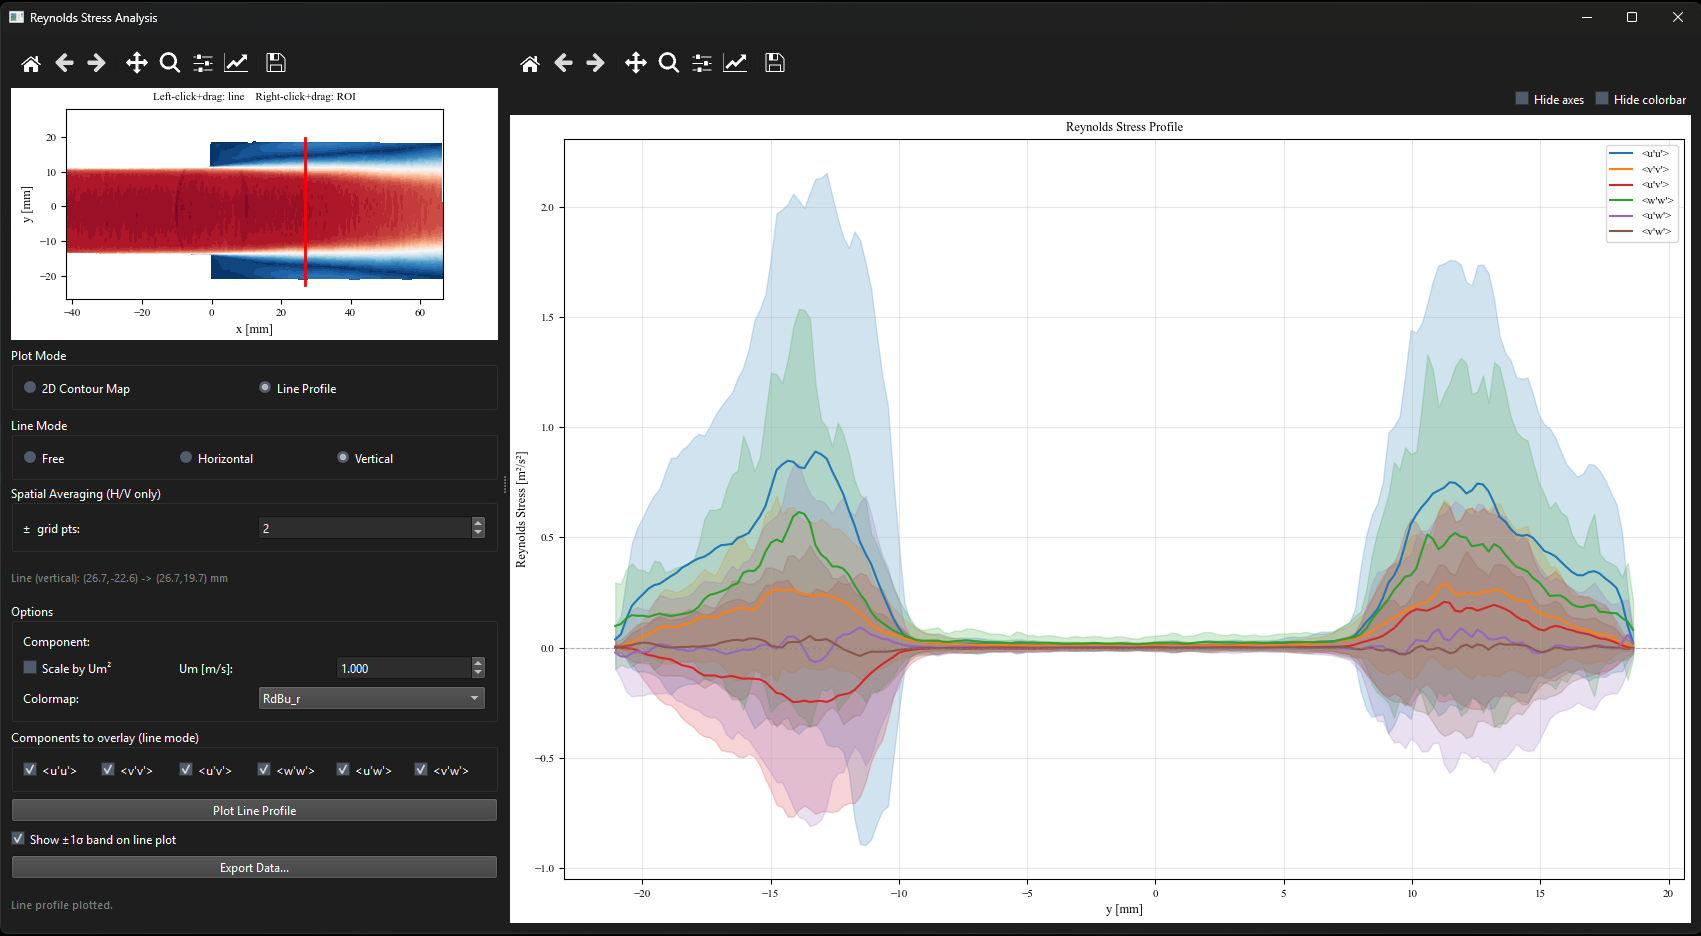
\includegraphics[width=0.92\linewidth]{fig3}
  \caption{Reynolds stress window in line profile mode. All stress components are plotted simultaneously in different colors. Optional shaded bands show $\pm 1\sigma$ statistical uncertainty (toggle in the side panel).}
  \label{fig:reynolds_profile}
\end{figure}

\section{Multi-case comparison}

The Reynolds Stress window supports importing CSV exports from previous sessions and overlaying them on the current plot. See Chapter~\ref{ch:multicase} for the full workflow. The same Import Case, Edit Styles, Manage Cases, and Export All Cases controls apply.

\section{Exporting}

Click \uipth{Export Data\ldots} to save all stress components simultaneously in a single Tecplot \texttt{.dat} file or as a CSV.

% ============================= CHAPTER 6 ==============================
\chapter{TKE Budget}
\label{ch:tke}

Open from \uipth{3.\ Analysis $\to$ TKE Budget}.

The turbulent kinetic energy $k = \tfrac{1}{2}\langle u'_i u'_i \rangle$ evolves according to the TKE transport equation (Pope, 2000, Ch.\ 5):
\[
\underbrace{\frac{\partial k}{\partial t}}_{\text{unsteady}} + \underbrace{\langle U_j \rangle \frac{\partial k}{\partial x_j}}_{C} = \underbrace{-\langle u'_i u'_j \rangle \frac{\partial \langle U_i \rangle}{\partial x_j}}_{P} \underbrace{- \frac{\partial}{\partial x_j}\!\left(\tfrac{1}{2}\langle u'_i u'_i u'_j \rangle + \frac{\langle p' u'_j \rangle}{\rho}\right)}_{D} - \underbrace{\nu \left\langle \frac{\partial u'_i}{\partial x_j}\frac{\partial u'_i}{\partial x_j} \right\rangle}_{\varepsilon}
\]

Production $P$ represents the rate at which turbulent energy is generated by the interaction of Reynolds stresses with the mean velocity gradients. Convection $C$ describes the transport of $k$ by the mean flow. Turbulent diffusion $D$ redistributes energy in space via triple velocity correlations. Viscous dissipation $\varepsilon$ converts kinetic energy irreversibly into heat at the small scales.

From planar PIV, the dissipation $\varepsilon$ and pressure diffusion cannot be computed directly. \software{uPrime} therefore computes a residual $R = P + D - C$ (for stationary turbulence with $\partial k/\partial t \approx 0$), which absorbs dissipation and any missing out-of-plane contributions. A non-zero $R$ is physically expected and is not an error.

Spatial gradients are computed using central differences with NaN-inpainting near mask boundaries to prevent spurious gradients at wall and shadow edges. Triple correlations for turbulent diffusion are optionally smoothed with a median filter before differentiation to reduce noise amplification.

\begin{notebox}
The residual $R$ absorbs pressure diffusion and viscous dissipation, which cannot be computed from planar PIV. A non-zero residual is expected and is \emph{not} an error in the calculation.
\end{notebox}

\noindent\textbf{Reference:} Pope, S.B. (2000). \textit{Turbulent Flows}. Cambridge University Press.

\begin{table}[htbp]
\centering
\caption{TKE budget terms in \software{uPrime}.}
\begin{tabular}{lll}
\toprule
\textbf{Symbol} & \textbf{Name} & \textbf{Availability} \\
\midrule
$k$                     & Turbulent kinetic energy  & Always \\
$P$                     & Production                & Always \\
$C$                     & Convection                & Always \\
$D$                     & Turbulent diffusion       & Always \\
$R$                     & Residual                  & Always \\
$\partial k/\partial t$ & Unsteady term             & TR data only \\
\bottomrule
\end{tabular}
\end{table}

\section{Using the window}

\begin{stepbox}
\begin{enumerate}[leftmargin=1.5em, topsep=2pt]
  \item Set parameters: enter $U_m$ and $L$ if normalising. Adjust the smoothing kernel if the field is noisy.
  \item Click \uipth{Compute Budget} (only needs to be done once per session).
  \item Select a term from the \uipth{Term} dropdown.
  \item Choose \uipth{2D Contour} or \uipth{Line Profile}.
  \item Click \uipth{Plot}.
\end{enumerate}
\end{stepbox}

In line profile mode, TKE $k$ is always overlaid as a dashed reference line regardless of which budget term is selected. Term-visibility checkboxes (\uipth{P}, \uipth{C}, \uipth{D}, \uipth{R}) below the plot control which budget terms appear. All four are checked by default; unchecking one hides it without recomputing.

\begin{figure}[htbp]
  \centering
  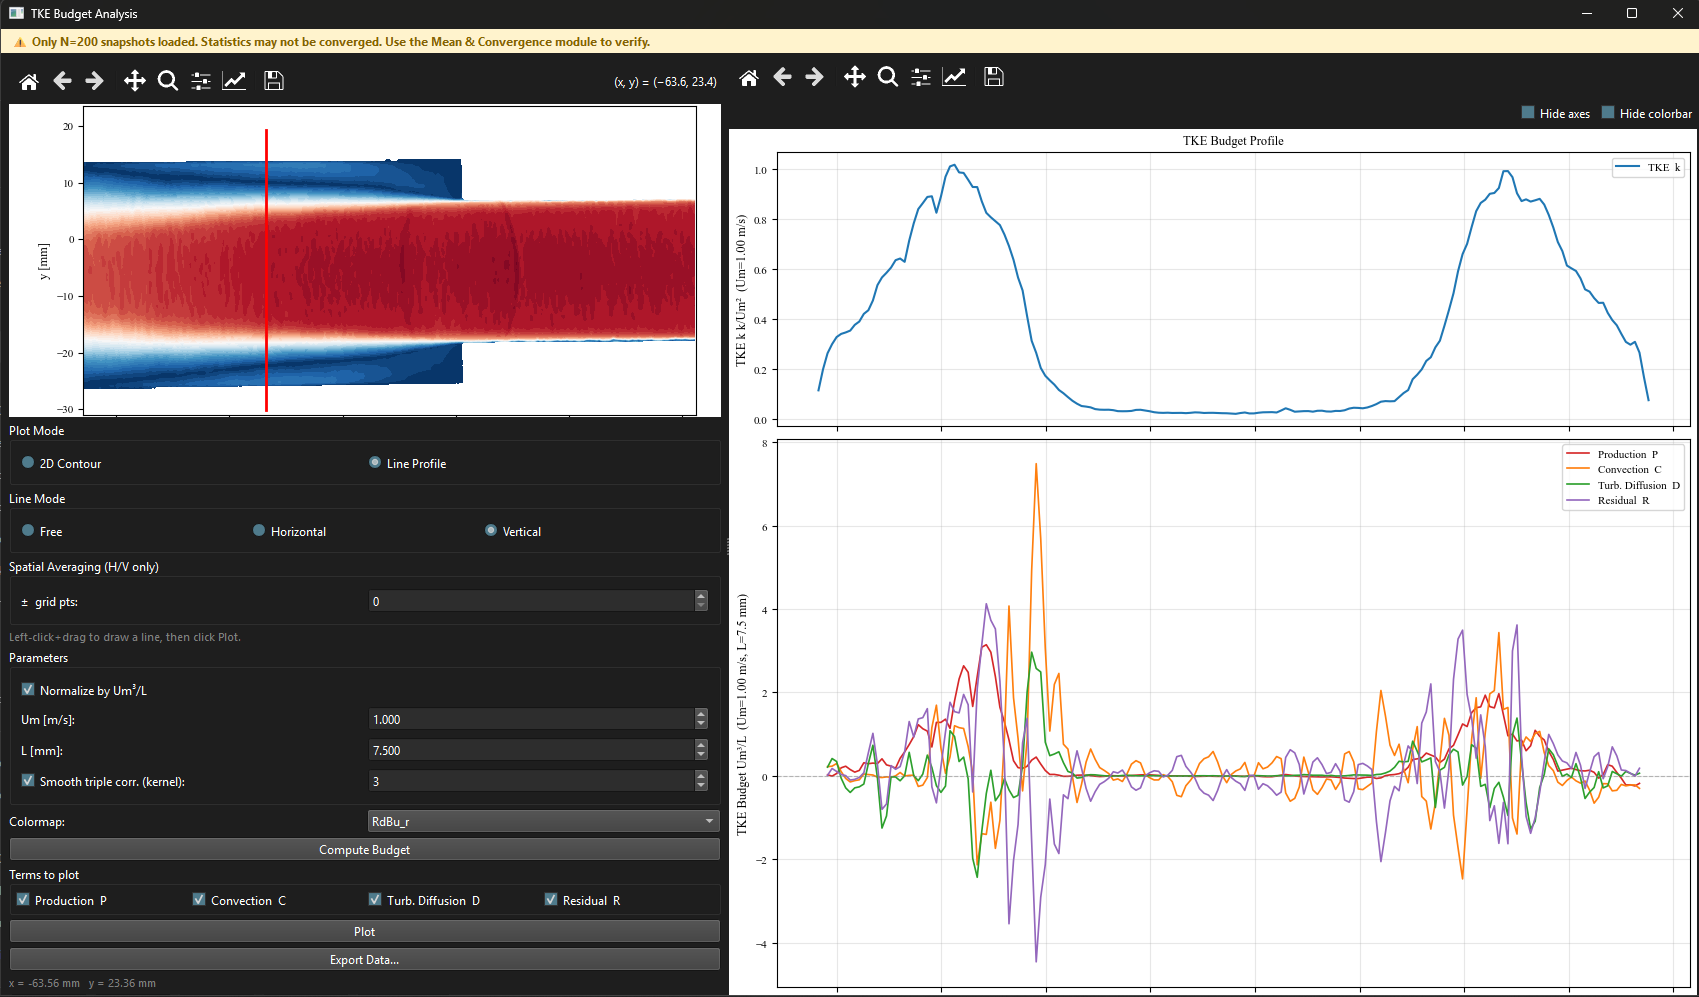
\includegraphics[width=0.92\linewidth]{fig_tke_terms}
  \caption{TKE Budget window in line profile mode showing $P$, $C$, $D$, $R$ along a vertical line through the shear layer. The four checkboxes below the plot control which terms are visible at any time. The mean field reference is shown in the left panel.}
  \label{fig:tkebudget}
\end{figure}

\begin{tipbox}
Enable \uipth{Normalize by $U_m^3/L$} to make the budget terms non-dimensional. TKE $k$ is normalized by $U_m^2$. This is essential when comparing results across different flow conditions or Reynolds numbers.
\end{tipbox}

\section{Multi-case comparison}

The TKE Budget window supports CSV import and overlay (Chapter~\ref{ch:multicase}).

\section{Exporting}

Click \uipth{Export Data\ldots} to save all budget terms together in a single file.

% ============================= CHAPTER 7 ==============================
\chapter{Space-Time Spectral Analysis}
\label{ch:spectra}

Open from \uipth{3.\ Analysis $\to$ Space-Time Spectra}.

The spectral window has four tabs. \textbf{Spatial (Welch)} is always available. \textbf{Temporal} and \textbf{Spatiotemporal} require time-resolved data. \textbf{Spatial (FFT)} is always available and provides a complementary 2D ROI-based spatial spectrum.

\section{Spatial Spectra -- Welch (Tab 1)}

The one-dimensional spatial energy spectrum $E(k)$ characterizes the distribution of turbulent kinetic energy across spatial scales. For homogeneous isotropic turbulence, Kolmogorov's similarity theory predicts an inertial subrange where $E(k) \propto k^{-5/3}$ (Kolmogorov, 1941). The spatial spectrum is computed along a user-defined line using Welch's method: the line is divided into overlapping segments, each Hann-windowed and Fourier-transformed, and the periodograms are averaged to reduce variance. The wavenumber $k$ is in rad/m.

\begin{stepbox}
\begin{enumerate}[leftmargin=1.5em, topsep=2pt]
  \item Choose \uipth{Horizontal ($k_x$)} or \uipth{Vertical ($k_y$)} mode.
  \item Left-click and drag on the field to draw the line.
  \item Select which velocity components to include (U, V, W).
  \item Set the number of Welch segments and overlap.
  \item Click \uipth{Compute}.
\end{enumerate}
\end{stepbox}

Results are plotted on a log-log scale. The Kolmogorov $-5/3$ reference slope can be toggled on/off. You can also compensate the spectrum by multiplying by $k^{5/3}$ to flatten the inertial range.

\begin{figure}[htbp]
  \centering
  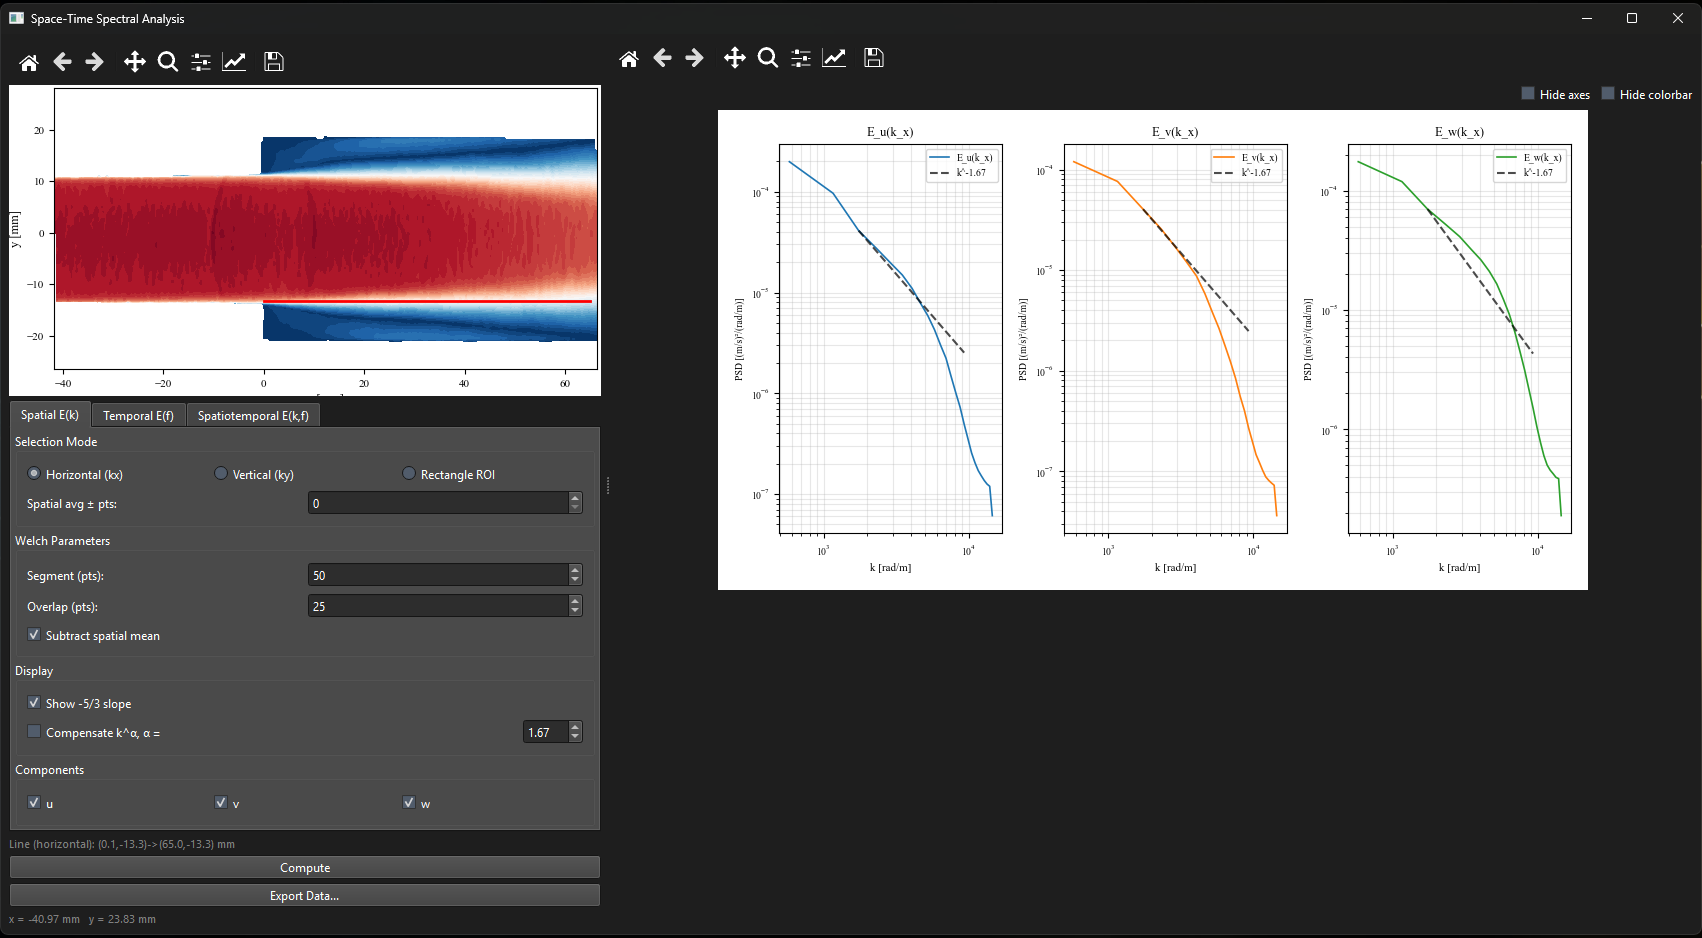
\includegraphics[width=0.92\linewidth]{fig5}
  \caption{Spatial spectra (Welch tab) showing $E(k_x)$ for the U and V components along a horizontal line through the shear layer. The dashed line shows the Kolmogorov $-5/3$ reference slope. The inertial subrange is visible between approximately $k = 100$ and $k = 1000$\,rad/m.}
  \label{fig:spectra}
\end{figure}

\noindent\textbf{Reference:} Kolmogorov, A.N. (1941). The local structure of turbulence in incompressible viscous fluid for very large Reynolds numbers. \textit{Proceedings of the USSR Academy of Sciences}, 30, 301--305.

\section{Temporal Spectra (Tab 2, TR Only)}

The power spectral density $E(f)$ of the velocity fluctuations at a fixed point reveals the temporal frequency content of the turbulence. Dominant peaks correspond to periodic or quasi-periodic phenomena such as vortex shedding, shear layer flapping, or acoustic resonances. The temporal spectrum is computed using Welch's method with a Hann window.

\begin{stepbox}
\begin{enumerate}[leftmargin=1.5em, topsep=2pt]
  \item Left-click on the field to pick a reference point, or right-click drag to draw an ROI.
  \item Set the number of Welch segments. More segments give a smoother spectrum at the cost of frequency resolution.
  \item Click \uipth{Compute}.
\end{enumerate}
\end{stepbox}

\begin{tipbox}
Looking for a shedding frequency or flapping mode? Use fewer segments (higher frequency resolution). Just want the spectral shape? Use more segments for a smoother curve.
\end{tipbox}

\section{Space-Time Spectra (Tab 3, TR Only)}

The two-dimensional space-time spectrum $E(k, f)$ jointly characterizes the spatial and temporal structure of convecting turbulent structures. It is computed by applying a 2D Fourier transform in both space (along a streamwise line) and time. Diagonal ridges in the resulting map correspond to spatially coherent structures convecting at a fixed speed. The slope of a ridge gives the convection velocity $U_c = 2\pi f / k$, providing a direct test of Taylor's frozen turbulence hypothesis (del \'{A}lamo \& Jim\'{e}nez, 2009).

\noindent\textbf{Reference:} del \'{A}lamo, J.C. \& Jim\'{e}nez, J. (2009). Estimation of turbulent convection velocities and corrections to Taylor's approximation. \textit{Journal of Fluid Mechanics}, 640, 5--26.

\section{Spatial Spectra -- FFT (Tab 4)}

Computes the 2D spatial energy spectrum over a rectangular ROI using a direct FFT (via pyFFTW), averaged over all snapshots. The result is shown as 1D marginal spectra $E(k_x)$ and $E(k_y)$ alongside the 2D spectral map.

\section{Multi-case comparison}

Spatial Welch and Temporal spectra support CSV import and overlay (Chapter~\ref{ch:multicase}).

% ============================= CHAPTER 8 ==============================
\chapter{Anisotropy Invariant Analysis}
\label{ch:anisotropy}

Open from \uipth{3.\ Analysis $\to$ Anisotropy Invariants}.

\begin{notebox}
This module requires \textbf{stereo PIV (2D3C)} data. It is not available for 2D2C datasets.
\end{notebox}

The Reynolds stress tensor $b_{ij} = \langle u'_i u'_j \rangle / (2k) - \delta_{ij}/3$ is a symmetric, traceless tensor that describes the anisotropy of the turbulence. Its eigenvalues $\lambda_1 \geq \lambda_2 \geq \lambda_3$ satisfy $\lambda_1 + \lambda_2 + \lambda_3 = 0$. The invariants of $b_{ij}$,
\[
\eta^2 = \frac{1}{6} b_{ij} b_{ji}, \qquad \xi^3 = \frac{1}{6} b_{ij} b_{jk} b_{ki},
\]
define a two-dimensional state space. All physically realizable turbulence states lie within the Lumley triangle, bounded by the one-component ($\lambda_1 = 2/3$), two-component ($\lambda_3 = -1/3$), and isotropic ($\lambda_i = 0$) limits (Lumley, 1978). The barycentric map is an alternative linear representation of the same anisotropy state space introduced by Banerjee et al.\ (2007), which maps the three limiting states to the vertices of an equilateral triangle with coordinates that vary linearly between limits.

\noindent\textbf{References:} Lumley, J.L. (1978). Computational modeling of turbulent flows. \textit{Advances in Applied Mechanics}, 18, 123--176. Banerjee, S., Krahl, R., Durst, F. \& Zenger, Ch. (2007). Presentation of anisotropy properties of turbulence. \textit{International Journal of Heat and Fluid Flow}, 28(3), 939--946.

\section{Lumley triangle mode}

\begin{stepbox}
\begin{enumerate}[leftmargin=1.5em, topsep=2pt]
  \item Ensure \uipth{Line (Lumley triangle)} is selected.
  \item Choose \uipth{Free}, \uipth{Horizontal}, or \uipth{Vertical} line orientation.
  \item Left-click and drag on the mean field to draw the sampling line.
  \item Click \uipth{Compute}.
\end{enumerate}
\end{stepbox}

Reading the triangle: the top vertex represents one-component turbulence; the bottom-left vertex represents two-component axisymmetric (disk-like) turbulence; the bottom-right vertex represents two-component axisymmetric (rod-like) turbulence; the origin represents isotropic turbulence. Points outside the boundary indicate numerical issues (insufficient snapshots or masked regions).

\begin{figure}[htbp]
  \centering
  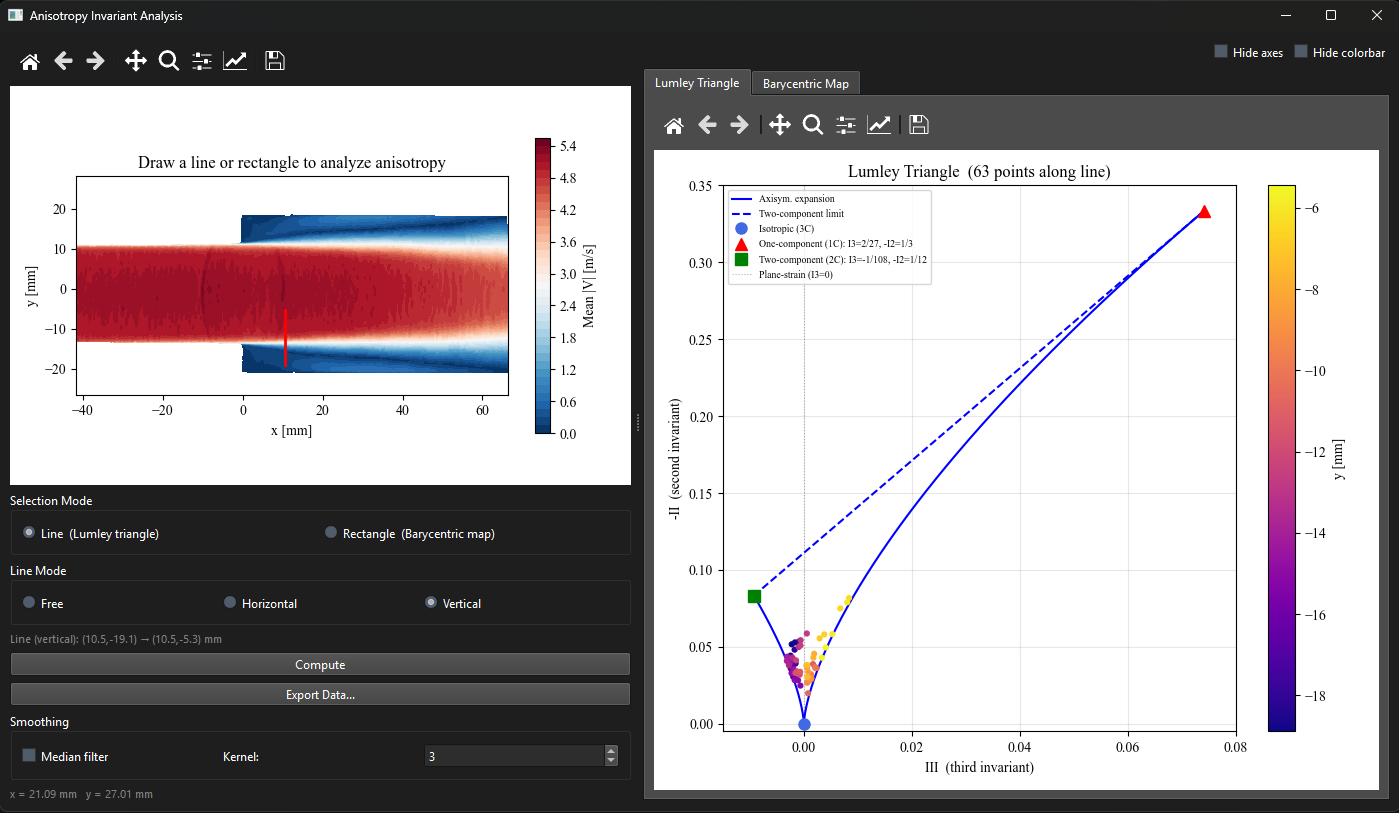
\includegraphics[width=0.92\linewidth]{fig7}
  \caption{Anisotropy window in Lumley triangle mode. Left: the vertical sampling line crosses the shear layer on the mean field. Right: each sampled point appears in the triangle, colored by its distance along the line. Points migrate from near-isotropic (center) toward the one-component vertex (top) inside the high-turbulence shear layer.}
  \label{fig:anisotropy}
\end{figure}

\section{Barycentric map mode}

\begin{stepbox}
\begin{enumerate}[leftmargin=1.5em, topsep=2pt]
  \item Select \uipth{Rectangle (Barycentric map)}.
  \item Left-click and drag to draw a rectangular region on the field.
  \item Click \uipth{Compute}.
\end{enumerate}
\end{stepbox}

The map colors each grid point by its anisotropy state: red = one-component, blue = two-component axisymmetric, green = three-component (near isotropic). Check \uipth{Median filter} to apply a $3\times3$ spatial smoothing to reduce noise.

\section{Multi-case comparison}

Lumley-triangle line profiles support CSV import and overlay (Chapter~\ref{ch:multicase}).

% ============================= CHAPTER 9 ==============================
\chapter{Correlation Analysis}
\label{ch:correlation}

Open from \uipth{3.\ Analysis $\to$ Correlation Analysis}.

The two-point spatial correlation function
\[
R_{uu}(\Delta x, \Delta y) = \frac{\langle u'(\mathbf{x}, t)\, u'(\mathbf{x}+\boldsymbol{\Delta}, t) \rangle}{\sigma(\mathbf{x})\,\sigma(\mathbf{x}+\boldsymbol{\Delta})}
\]
measures the degree to which velocity fluctuations at two different locations are statistically related. When $R_{uu}$ decays from 1 at $\Delta = 0$ to 0, the separation at which it crosses zero defines the integral length scale $L$, a measure of the size of the largest energy-containing eddies (Pope, 2000). The temporal autocorrelation $R(\tau)$ plays an analogous role in time, with the integral time scale $T = \int_0^{\infty} R(\tau)\,\mathrm{d}\tau$.

\noindent\textbf{Reference:} Pope, S.B. (2000). \textit{Turbulent Flows}. Cambridge University Press.

\section{Selecting a reference}

\begin{itemize}[leftmargin=1.5em]
  \item \uipth{Point mode}: left-click on the mean field to select a single reference point. Enable \uipth{$3\times3$ kernel average} to reduce sensitivity to noisy vectors at that point.
  \item \uipth{ROI mode}: left-click and drag to draw a rectangle. The correlation is computed as a spatial average over the region.
\end{itemize}

\section{Spatial correlation}

\begin{stepbox}
\begin{enumerate}[leftmargin=1.5em, topsep=2pt]
  \item Select Point or ROI mode and pick your reference on the field.
  \item Choose the velocity component: R$_{uu}$, R$_{vv}$, or R$_{ww}$.
  \item Select the \uipth{Scale method} (Table~\ref{tab:scalemethods}).
  \item Click \uipth{Compute Spatial Correlation}.
\end{enumerate}
\end{stepbox}

In Point mode you see the full 2D correlation map and two independent 1D slice panels. In ROI mode only the 1D panels are shown. The computed $L_x$ and $L_y$ are displayed in the readout strip at the bottom of the window. A vertical dashed line marks the crossing lag used by the selected scale method; for the zero-crossing method, this line is placed at the lag where $R$ first crosses zero, while $L$ is reported as the integral of $R$ up to that crossing. Click \uipth{Show Diagnostic Plot} to see the cumulative integral of $R(\Delta r)$.

\begin{figure}[htbp]
  \centering
  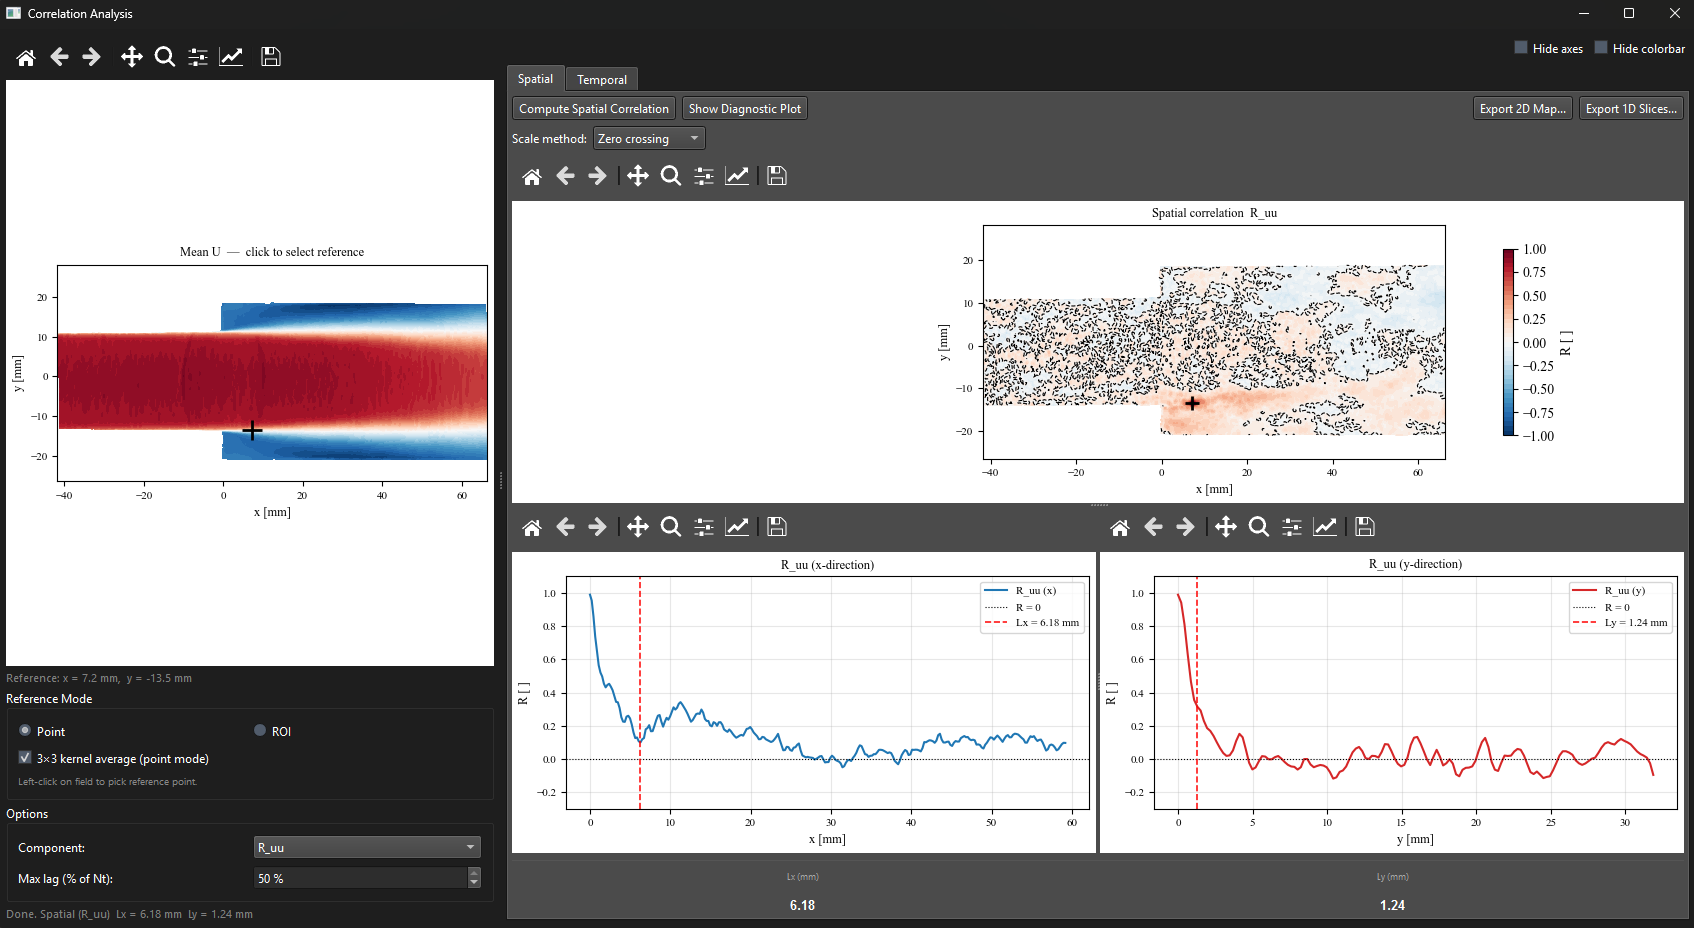
\includegraphics[width=0.92\linewidth]{fig6}
  \caption{Correlation window in ROI mode showing $R_{uu}$ in the $x$- and $y$-directions. The vertical dashed red line marks the zero-crossing lag used to compute the integral length scale. $L_x$ and $L_y$ are reported in the readout strip at the bottom.}
  \label{fig:correlation}
\end{figure}

\begin{table}[htbp]
\centering
\caption{Integral scale methods.}
\label{tab:scalemethods}
\begin{tabular}{lp{9cm}}
\toprule
\textbf{Method} & \textbf{When to use} \\
\midrule
Zero crossing   & Clean, well-resolved correlations with a clear zero crossing. Standard choice. \\
Exponential fit & Noisy correlations without a clear zero crossing. Robust to noise in the tail. \\
1/e point       & Returns the lag at which $R$ first drops to $e^{-1} \approx 0.368$ (interpolated). \\
Domain integral & When no zero crossing exists and you want a conservative upper bound. \\
\bottomrule
\end{tabular}
\end{table}

\begin{tipbox}
If unsure, start with \textbf{Zero crossing}. If the correlation does not have a clean crossing (common for low-Reynolds-number flows or short datasets), switch to \textbf{Exponential fit}.
\end{tipbox}

\section{Temporal correlation (TR only)}

\begin{stepbox}
\begin{enumerate}[leftmargin=1.5em, topsep=2pt]
  \item Click the \uipth{Temporal} tab.
  \item Pick a reference point or draw an ROI as before.
  \item Set \uipth{Max lag (\% of Nt)}: 50\% is usually sufficient.
  \item Select the Scale method.
  \item Click \uipth{Compute Temporal Correlation}.
\end{enumerate}
\end{stepbox}

Results show $R(\tau)$ vs time lag $\tau$ in milliseconds, with integral time scale $T$ and Taylor microscale $\lambda_t$ marked.

\section{Multi-case comparison}

Spatial 1D slice and temporal correlation curves support CSV import and overlay (Chapter~\ref{ch:multicase}).

% ============================= CHAPTER 10 ==============================
\chapter{POD Analysis}
\label{ch:pod}

Open from \uipth{3.\ Analysis $\to$ POD Analysis}.

Proper Orthogonal Decomposition (POD) finds the most efficient low-dimensional representation of the velocity field by decomposing the fluctuation field into a set of orthogonal spatial modes $\boldsymbol{\phi}_n(\mathbf{x})$ and corresponding temporal coefficients $a_n(t)$:
\[
\mathbf{u}'(\mathbf{x}, t) = \sum_{n=1}^{N} a_n(t)\,\boldsymbol{\phi}_n(\mathbf{x})
\]
The modes are ordered by their energy content: Mode 1 captures the largest fraction of the total TKE, Mode 2 the next largest, and so on. This property, known as optimality, means that the POD is the most efficient basis for representing the flow in a least-squares sense (Lumley, 1967; Holmes et al., 1996). In practice, a small number of modes often captures the dominant coherent structures (recirculation zones, vortex shedding, shear layer flapping), while the remaining modes represent incoherent noise.

\software{uPrime} implements the snapshot POD method (Sirovich, 1987), which is efficient when the number of spatial grid points exceeds the number of snapshots. The SVD of the fluctuation snapshot matrix directly yields the POD modes and their energy content.

\noindent\textbf{References:} Lumley, J.L. (1967). The structure of inhomogeneous turbulent flows. In \textit{Atmospheric Turbulence and Radio Wave Propagation}, 166--178. Holmes, P., Lumley, J.L. \& Berkooz, G. (1996). \textit{Turbulence, Coherent Structures, Dynamical Systems and Symmetry}. Cambridge University Press. Sirovich, L. (1987). Turbulence and the dynamics of coherent structures. \textit{Quarterly of Applied Mathematics}, 45(3), 561--590.

\section{Computing POD}

\begin{stepbox}
\begin{enumerate}[leftmargin=1.5em, topsep=2pt]
  \item Set \uipth{Modes to compute} (default 25). Increasing this takes longer.
  \item Click \uipth{Compute POD}. For large datasets this may take several seconds to a minute.
  \item All four tabs populate automatically when done.
\end{enumerate}
\end{stepbox}

\begin{notebox}
POD uses all velocity components simultaneously (U+V for 2D2C; U+V+W for 2D3C). The energy percentage of each mode reflects the combined energy across all components.
\end{notebox}

\section{Energy Spectrum tab}

Use the energy spectrum to decide how many modes to use for reconstruction and interpretation. A steep drop after Mode 1 or 2 indicates a flow dominated by one or two strong coherent structures. A slow gradual decay indicates broadband turbulence with energy distributed across many scales.

\begin{figure}[htbp]
  \centering
  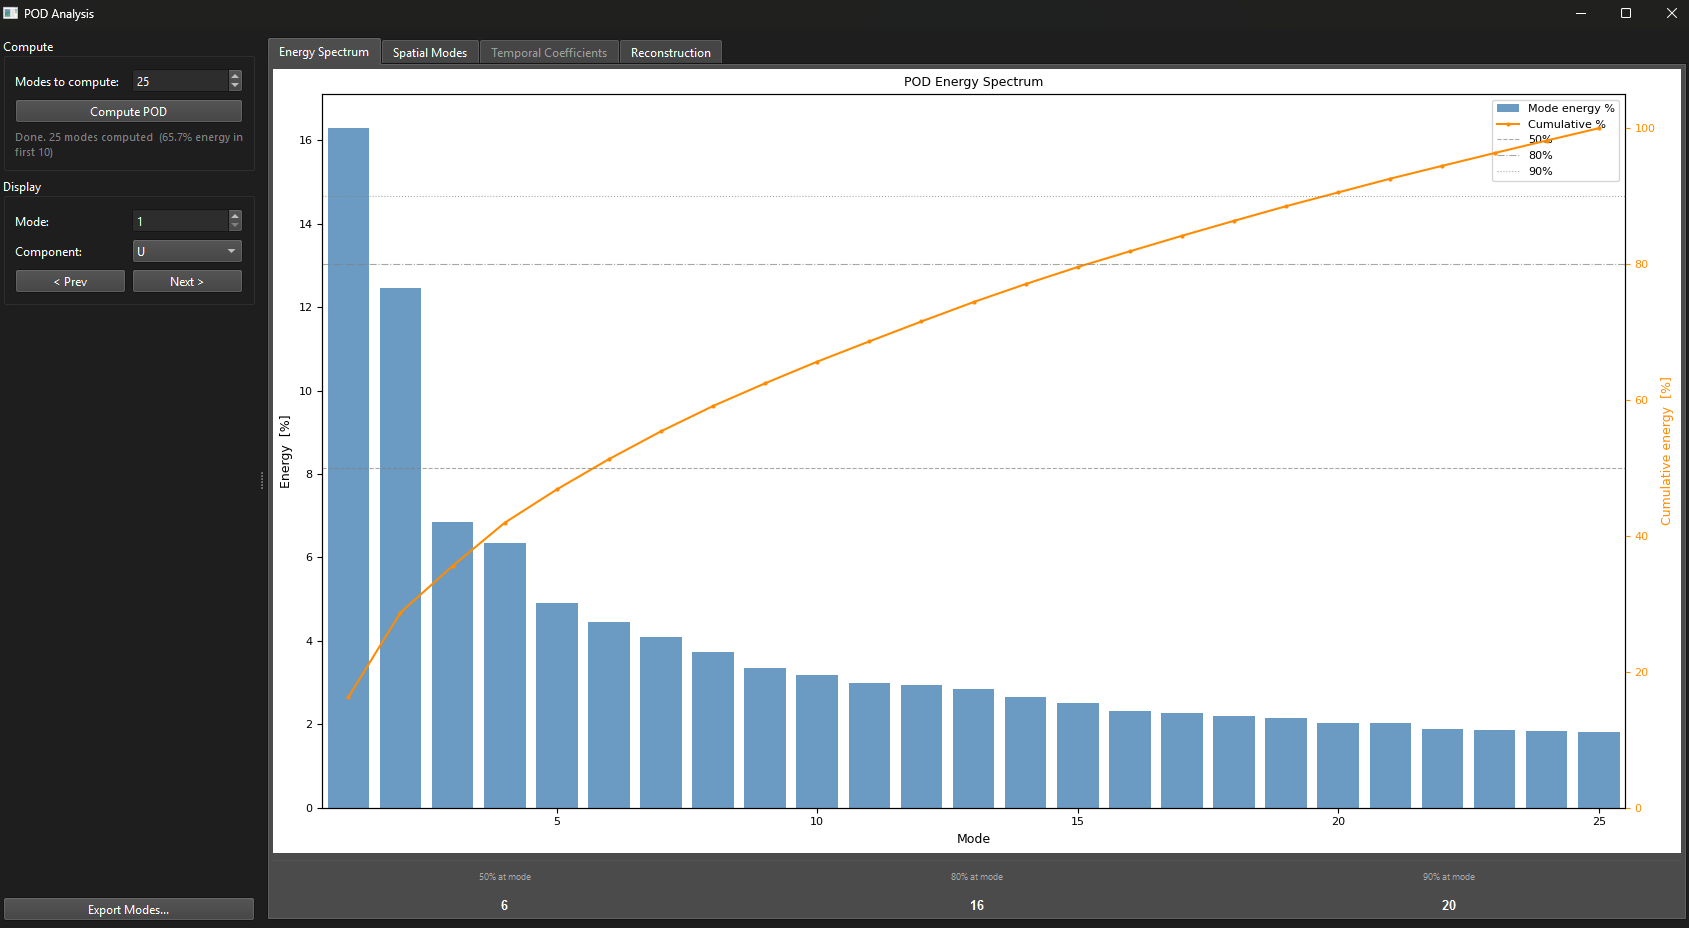
\includegraphics[width=0.92\linewidth]{fig8}
  \caption{POD Energy Spectrum tab. Bars show the energy percentage per mode; the orange curve shows cumulative energy. Dashed horizontal lines mark the 50\%, 80\%, and 90\% thresholds. The readout strip at the bottom shows how many modes are needed to reach each threshold.}
  \label{fig:pod_energy}
\end{figure}

\section{Spatial Modes tab}

Use the \uipth{Mode} spinbox or \uipth{$<$ Prev} / \uipth{Next $>$} buttons to step through modes. Use the \uipth{Component} dropdown to inspect different velocity directions. The title shows the mode number and its energy fraction.

\begin{figure}[htbp]
  \centering
  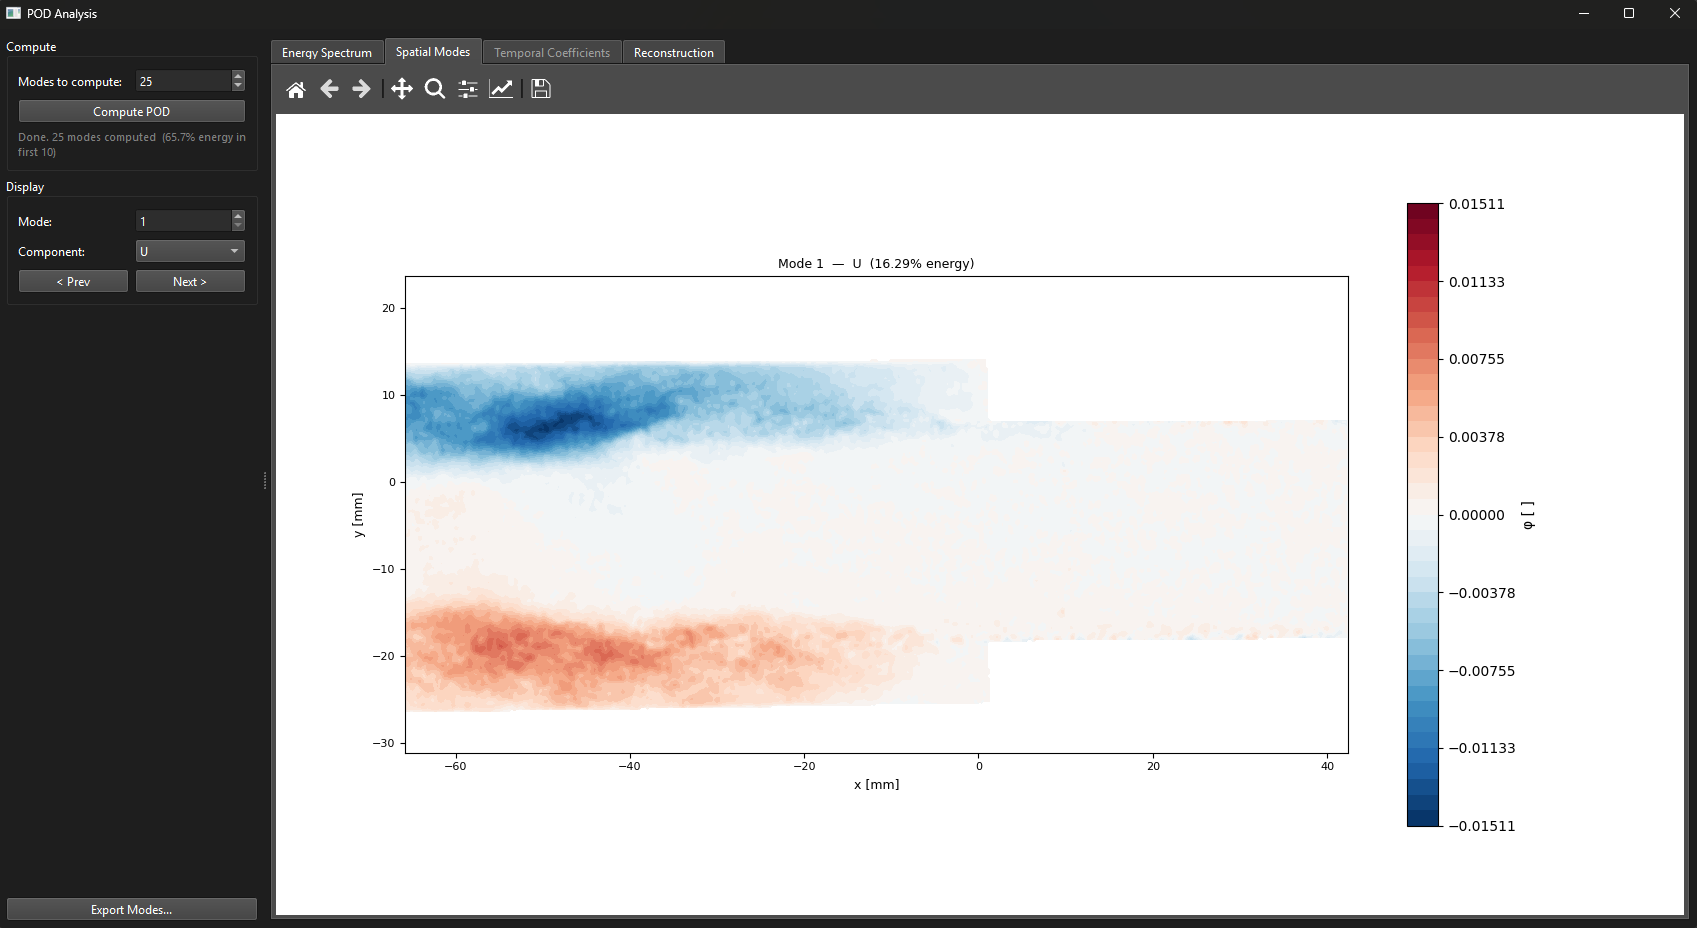
\includegraphics[width=0.92\linewidth]{fig9}
  \caption{POD Spatial Modes tab showing Mode~1 of the $U$ component. Red and blue regions represent opposite-signed velocity fluctuations associated with the dominant coherent structure in the flow. The energy fraction of the mode is shown in the plot title.}
  \label{fig:pod_mode}
\end{figure}

\section{Temporal Coefficients tab (TR only)}

Shows the temporal coefficient time series $a_n(t)$ for the selected mode and its power spectral density. A sharp peak in the PSD indicates a periodic structure at that frequency (e.g.\ vortex shedding or shear layer flapping).

\section{Reconstruction tab}

\begin{figure}[htbp]
  \centering
  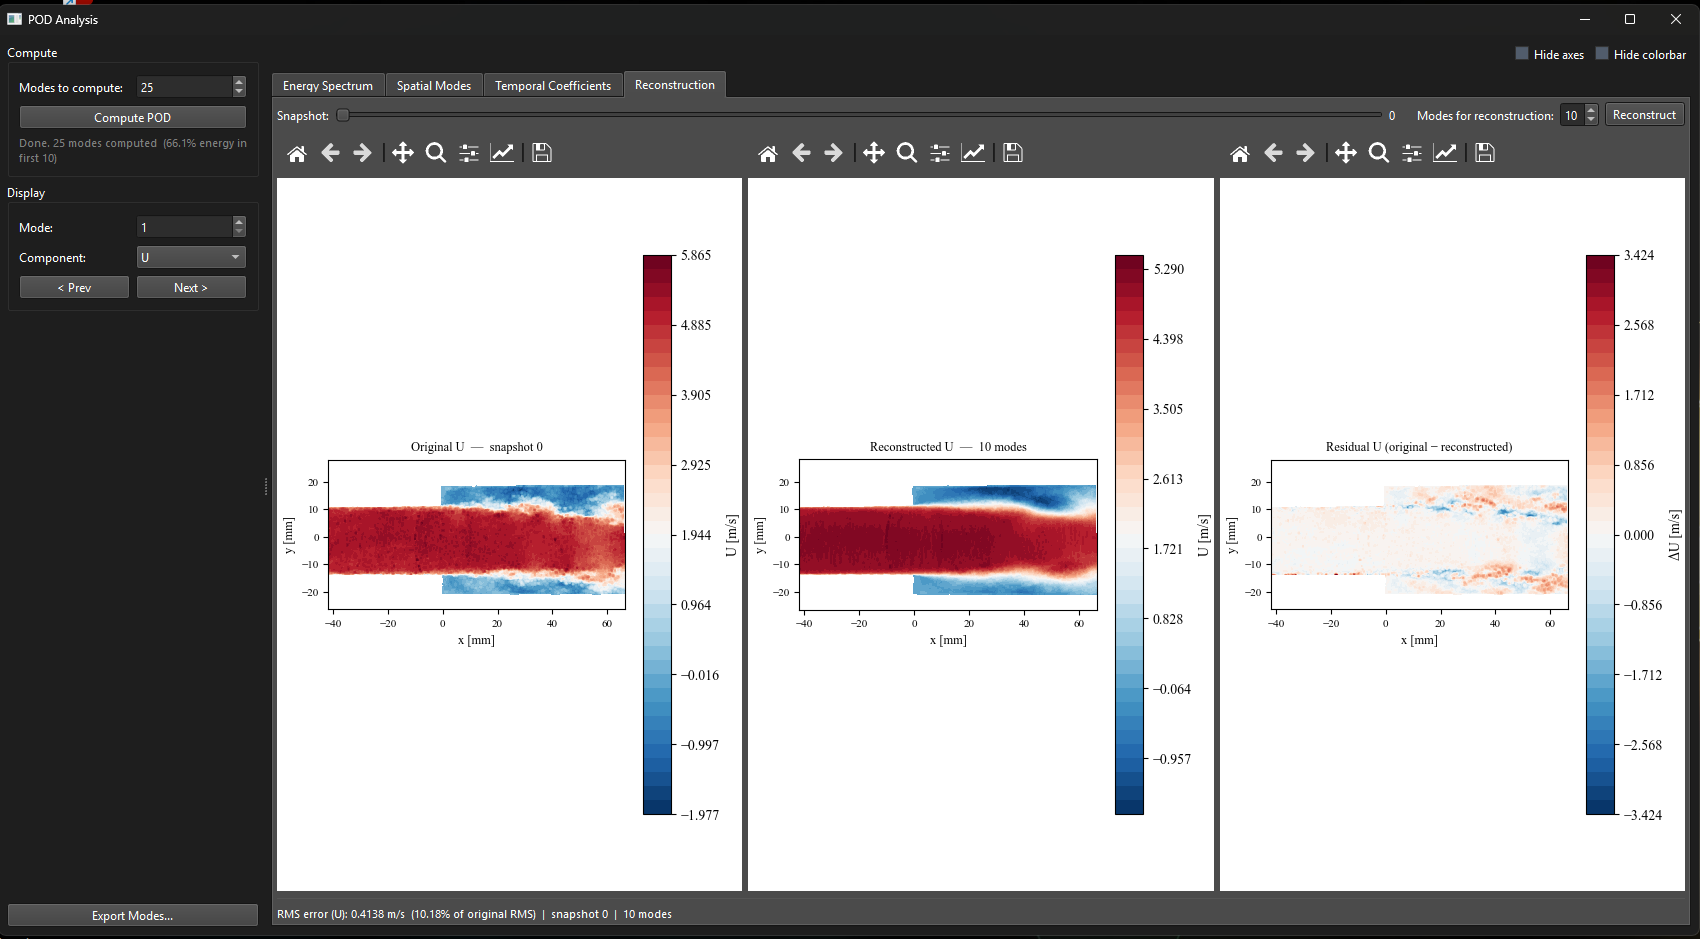
\includegraphics[width=0.92\linewidth]{fig10}
  \caption{POD Reconstruction tab. Left: original snapshot. Center: low-order reconstruction with selected modes. Right: residual (original minus reconstructed). The RMS reconstruction error is shown at the bottom.}
  \label{fig:pod_recon}
\end{figure}

\begin{stepbox}
\begin{enumerate}[leftmargin=1.5em, topsep=2pt]
  \item Drag the \uipth{Snapshot} slider to select a snapshot.
  \item Set \uipth{Modes for reconstruction} (minimum 1).
  \item Click \uipth{Reconstruct}.
\end{enumerate}
\end{stepbox}

The three panels show the original field, the low-order reconstruction, and the residual. A residual below 10--20\% RMS generally means the selected modes capture the dominant structure.

\section{Exporting}

Click \uipth{Export Modes\ldots} to save all spatial modes as a Tecplot \texttt{.dat} file and temporal coefficients as a \texttt{.csv} file.

% ============================= CHAPTER 11 ==============================
\chapter{DMD Analysis}
\label{ch:dmd}

Open from \uipth{3.\ Analysis $\to$ DMD Analysis}.

\begin{notebox}
DMD requires \textbf{time-resolved} data and at least 50 snapshots. The button is greyed out for non-TR datasets.
\end{notebox}

Dynamic Mode Decomposition (DMD) extracts spatial modes that oscillate at a single frequency and grow or decay at a single rate. Unlike POD, DMD modes are not ordered by energy but by their dynamic content. This makes DMD ideal for isolating periodic phenomena such as vortex shedding, acoustic resonances, or shear layer flapping (Schmid, 2010; Tu et al., 2014).

\noindent\textbf{References:} Schmid, P.J. (2010). Dynamic mode decomposition of numerical and experimental data. \textit{Journal of Fluid Mechanics}, 656, 5--28. Tu, J.H., Rowley, C.W., Luchtenburg, D.M., Brunton, S.L. \& Kutz, J.N. (2014). On dynamic mode decomposition: theory and applications. \textit{Journal of Computational Dynamics}, 1(2), 391--421.

\section{Computing DMD}

\begin{stepbox}
\begin{enumerate}[leftmargin=1.5em, topsep=2pt]
  \item Set \uipth{Rank truncation} (default 50). This caps the number of DMD modes.
  \item Optionally enable a Strouhal number normalization with a reference length and velocity.
  \item Click \uipth{Compute DMD}.
\end{enumerate}
\end{stepbox}

\section{Spectrum tab}

The spectrum shows each DMD mode as a bubble in the frequency-growth-rate plane, with bubble area proportional to mode amplitude. Click on any bubble to display its spatial structure in the Mode tab. A growth-rate filter $|\sigma| < $ threshold can be applied to focus on near-neutral physically meaningful modes.

\section{Mode tab}

Displays the spatial structure (real and imaginary parts) of the currently selected DMD mode for the chosen velocity component.

\begin{figure}[htbp]
  \centering
  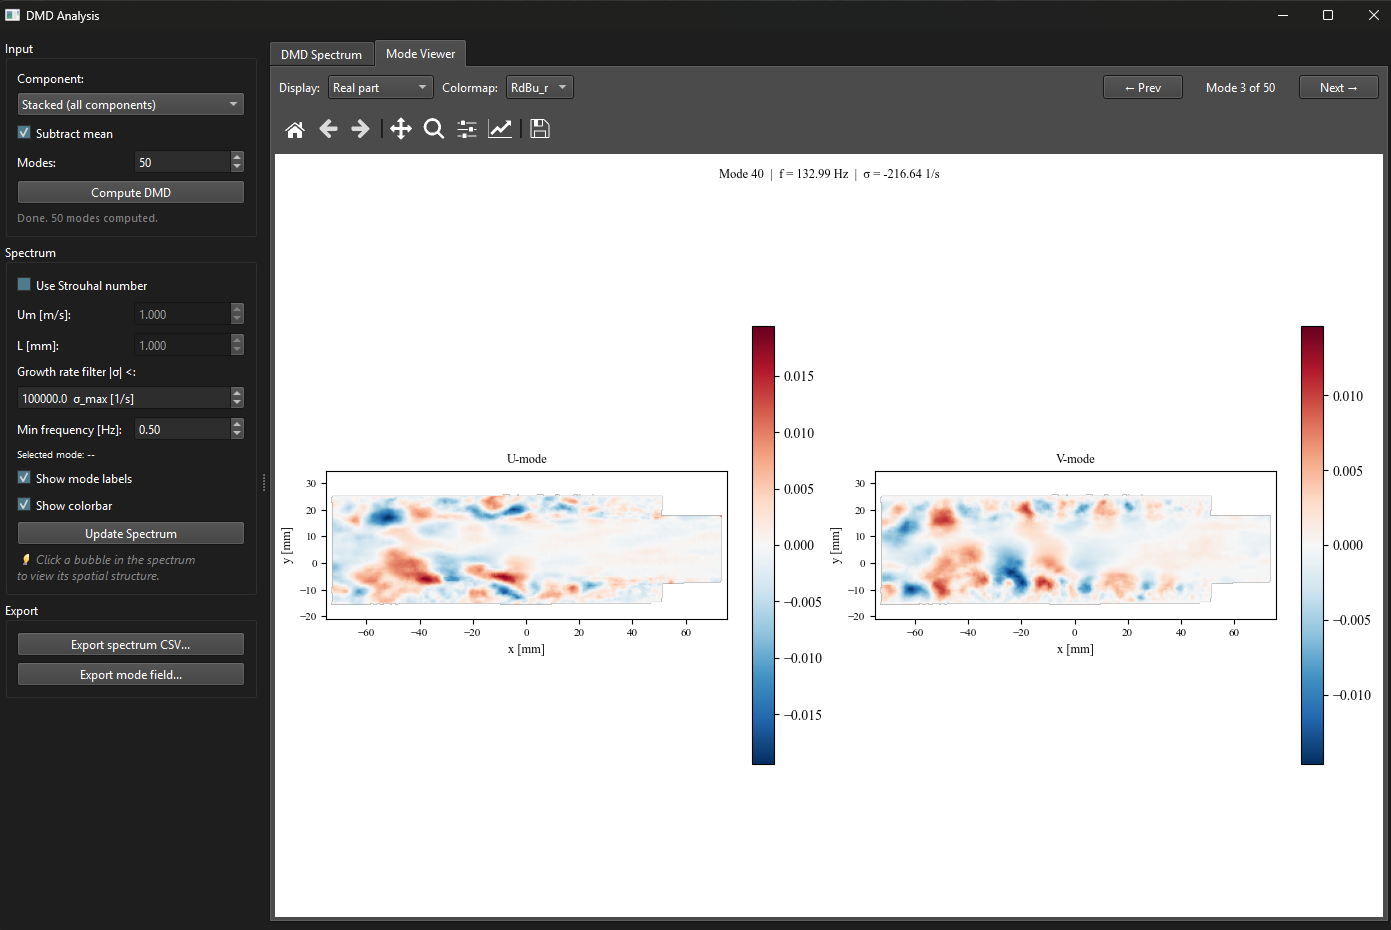
\includegraphics[width=0.92\linewidth]{fig_dmd_mode}
  \caption{DMD Mode tab showing the real and imaginary parts of a selected mode. Animating between them gives a sense of the structure's oscillation in time.}
  \label{fig:dmd_mode}
\end{figure}

\begin{tipbox}
The real and imaginary parts of a DMD mode represent the two phases of the oscillation separated by a quarter period. Animating between them (real $\to$ imaginary $\to$ $-$real $\to$ $-$imaginary) gives a physical sense of how the structure evolves in time.
\end{tipbox}

\section{Exporting}

Click \uipth{Export spectrum CSV\ldots} to save a table of all modes with their frequency, growth rate, and amplitude. Click \uipth{Export mode field\ldots} to save the spatial structure of the currently selected mode as a Tecplot \texttt{.dat} file.

% ============================= CHAPTER 12 ==============================
\chapter{Vortex Identification}
\label{ch:vortex}

Open from \uipth{3.\ Analysis $\to$ Vortex Identification}.

Vortex identification methods seek to objectively define the boundary and core of a vortex from the instantaneous or mean velocity field. \software{uPrime} implements five scalar criteria, which can be broadly divided into gradient-based (Eulerian) methods and the integral-based Graftieaux criteria.

\subsection*{Gradient-based methods}

All four gradient-based methods derive from the 2D velocity gradient tensor:
\[
\nabla \mathbf{u} = \begin{pmatrix} \partial u/\partial x & \partial u/\partial y \\ \partial v/\partial x & \partial v/\partial y \end{pmatrix}
\]
which is decomposed into its symmetric strain rate $\mathbf{S} = \tfrac{1}{2}(\nabla\mathbf{u} + \nabla\mathbf{u}^\top)$ and antisymmetric rotation rate $\boldsymbol{\Omega} = \tfrac{1}{2}(\nabla\mathbf{u} - \nabla\mathbf{u}^\top)$.

\begin{itemize}[leftmargin=1.5em]
  \item \textbf{Vorticity} $\omega = \partial v/\partial x - \partial u/\partial y$: the simplest measure of local rotation, but nonzero in shear layers even without a vortex core.

  \item \textbf{Q-criterion} (Hunt et al., 1988): $Q = -\tfrac{1}{2}(\partial_x u^2 + \partial_y v^2 + 2\,\partial_y u\,\partial_x v)$. A vortex core is identified where $Q > 0$, meaning rotation dominates strain. Q is the most widely used criterion in PIV literature.

  \item \textbf{Swirling strength} $\lambda_{ci}$ (Zhou et al., 1999): the imaginary part of the complex eigenvalue of $\nabla\mathbf{u}$. Complex eigenvalues exist only where the flow is locally swirling; $\lambda_{ci}$ is therefore immune to pure shear contamination that inflates $\omega$ and $Q$ in shear layers. \software{uPrime} multiplies by $\text{sign}(\omega)$ to retain rotation direction.

  \item \textbf{$\lambda_2$-criterion} (Jeong \& Hussain, 1995): identifies a vortex core as a connected region where the second eigenvalue of $\mathbf{S}^2 + \boldsymbol{\Omega}^2$ is negative. This criterion has a direct physical motivation: $\lambda_2 < 0$ marks regions where the centrifugal tendency of the pressure field overcomes both strain and unsteady effects.
\end{itemize}

\noindent\textbf{References:} Hunt, J.C.R., Wray, A. \& Moin, P. (1988). Eddies, stream, and convergence zones in turbulent flows. \textit{CTR Report CTR-S88}, 193--208. Zhou, J., Adrian, R.J., Balachandar, S. \& Kendall, T.M. (1999). Mechanisms for generating coherent packets of hairpin vortices in channel flow. \textit{Journal of Fluid Mechanics}, 387, 353--396. Jeong, J. \& Hussain, F. (1995). On the identification of a vortex. \textit{Journal of Fluid Mechanics}, 285, 69--94.

\subsection*{Graftieaux $\Gamma$ functions}

The $\Gamma$ functions (Graftieaux et al., 2001) are computed directly from the velocity vectors without differentiation, making them substantially more robust to PIV measurement noise:
\[
\Gamma_1(P) = \frac{1}{N} \sum_{M \in \mathcal{S}} \sin\!\left(\widehat{\mathbf{PM},\, \mathbf{U}_M}\right), \qquad
\Gamma_2(P) = \frac{1}{N} \sum_{M \in \mathcal{S}} \sin\!\left(\widehat{\mathbf{PM},\, \mathbf{U}_M - \widetilde{\mathbf{U}}}\right)
\]
where $\mathcal{S}$ is a local neighborhood of $N$ points around $P$, $\widehat{(\cdot,\cdot)}$ denotes the angle between two vectors, and $\widetilde{\mathbf{U}}$ is the local mean velocity over $\mathcal{S}$. Both functions are bounded between $-1$ and $+1$. The sign gives the rotation direction ($+1$ = CCW, $-1$ = CW). A vortex \emph{core} is identified where $|\Gamma_1| > 0.6$--$0.7$; the vortex \emph{boundary} is where $|\Gamma_2| > 2/\pi \approx 0.64$. The neighborhood half-width $S$ (default 2, corresponding to a $5 \times 5$ stencil) is user-adjustable.

\noindent\textbf{Reference:} Graftieaux, L., Michard, M. \& Grosjean, N. (2001). Combining PIV, POD and vortex identification algorithms for the study of unsteady turbulent swirling flows. \textit{Measurement Science and Technology}, 12(9), 1422--1429.

\section{Field View tab}

\begin{stepbox}
\begin{enumerate}[leftmargin=1.5em, topsep=2pt]
  \item Select the scalar field and input (mean or instantaneous frame).
  \item Click \uipth{Compute Field}.
  \item Set the threshold fraction and sign filter, then click \uipth{Detect Vortices}.
  \item Check \uipth{Show vortex boundaries} to overlay detected contours on the colormap.
\end{enumerate}
\end{stepbox}

The threshold is expressed as a fraction of the field maximum, making it dataset-agnostic. The actual physical value is shown in the readout next to the slider. For the $\Gamma$ criteria the threshold has a universal meaning ($|\Gamma_1| = 0.6$ corresponds to the standard core boundary); for gradient-based criteria it is dataset-dependent and must be chosen by the user.

\begin{figure}[htbp]
  \centering
  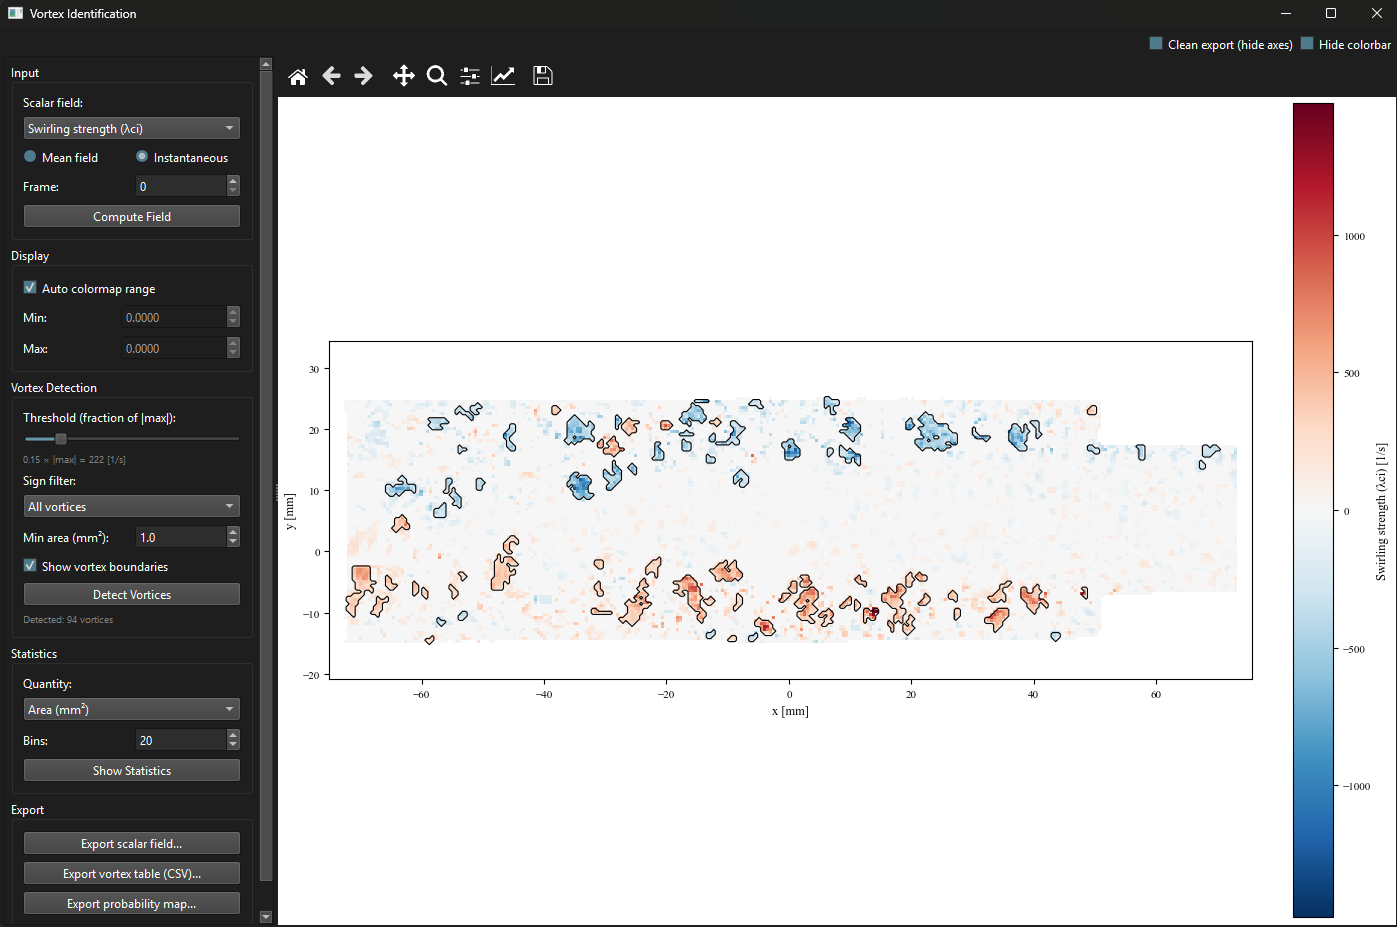
\includegraphics[width=0.92\linewidth]{fig_vortex_field}
  \caption{Vortex Identification window showing the swirling strength $\lambda_{ci}$ field for an instantaneous snapshot. Detected vortex boundaries (black contour lines) are overlaid on the colormap. The threshold is set to 15\% of the field maximum. Red regions indicate positive (CCW) rotation; blue regions indicate negative (CW) rotation. A total of 94 vortices are detected above the minimum area threshold.}
  \label{fig:vortex_field}
\end{figure}

\begin{tipbox}
For PIV data, start with $\Gamma_1/\Gamma_2$, which is most robust to measurement noise. Cross-check with Q-criterion or $\lambda_{ci}$. If the two methods agree, the detected structures are reliable.
\end{tipbox}

\section{Vortex Statistics tab}

After clicking \uipth{Show Statistics}, two plots appear: a spatial probability map showing how often a vortex is detected at each grid point across all snapshots, and a histogram of the selected per-vortex quantity (area, circulation, or aspect ratio) with positive and negative vortices shown separately in red and blue.

\begin{figure}[htbp]
  \centering
  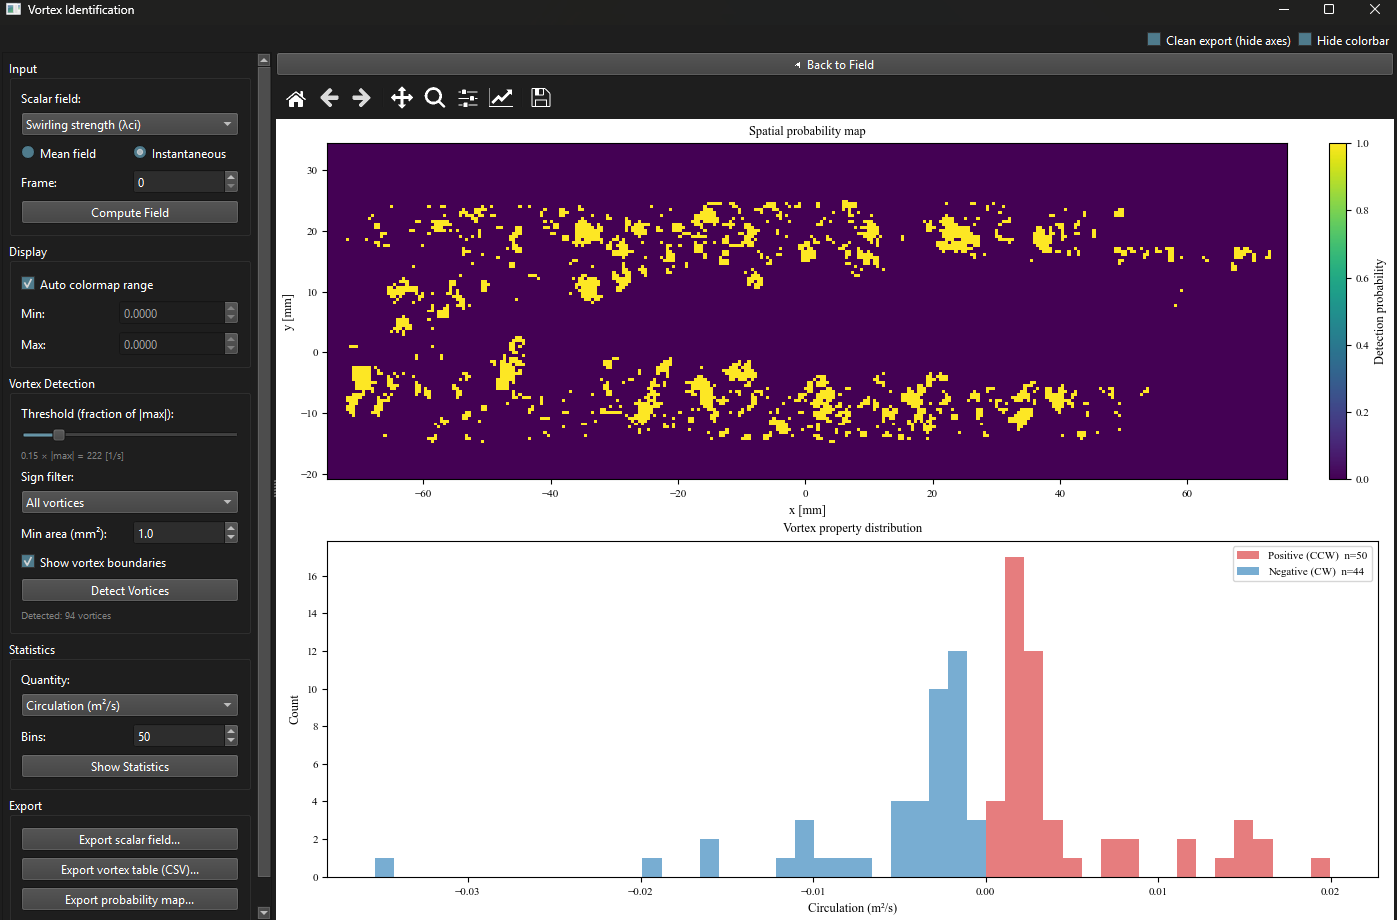
\includegraphics[width=0.92\linewidth]{fig_vortex_stats}
  \caption{Vortex Statistics view. Top: spatial probability map showing the fraction of snapshots in which a vortex is detected at each grid point (viridis colormap, 0--1). Yellow regions indicate persistent vortex locations concentrated in the shear layers. Bottom: circulation histogram for 94 detected vortices (50 CCW in red, 44 CW in blue). The near-symmetric distribution about zero is consistent with a turbulent shear layer with no mean rotation bias.}
  \label{fig:vortex_stats}
\end{figure}

\section{Exporting}

Click \uipth{Export scalar field\ldots} to save the scalar field as a Tecplot \texttt{.dat} file. Click \uipth{Export vortex table (CSV)\ldots} to save a per-vortex table with columns: vortex ID, centroid position, area, sign, circulation, aspect ratio, and frame index. The default filename now reflects the active criterion (e.g.\ \texttt{vortex\_lambda\_ci\_dataset.csv}). This CSV is designed to be imported into post-processing scripts for vortex tracking or further statistical analysis.

% ============================= CHAPTER 13 ==============================
\chapter{Multi-case Comparison}
\label{ch:multicase}

Several analysis modules support importing CSV files from previous \software{uPrime} sessions and overlaying them on top of the current plot. This is useful for comparing experimental conditions, validating against numerical data, or assembling multi-panel publication figures.

The same workflow is used in: Mean \& Convergence (Mean Velocity tab), Reynolds Stress, TKE Budget, Spectra (Spatial Welch and Temporal), Correlation, and Anisotropy (Lumley line mode).

\section{Importing a case}

Click \uipth{Import Case\ldots} and select a CSV file. The CSV must follow the column layout produced by \software{uPrime}'s own \uipth{Export Profile} or \uipth{Export Data} actions. The imported case is added to the case list with an auto-assigned color and dashed linestyle.

\begin{figure}[htbp]
  \centering
  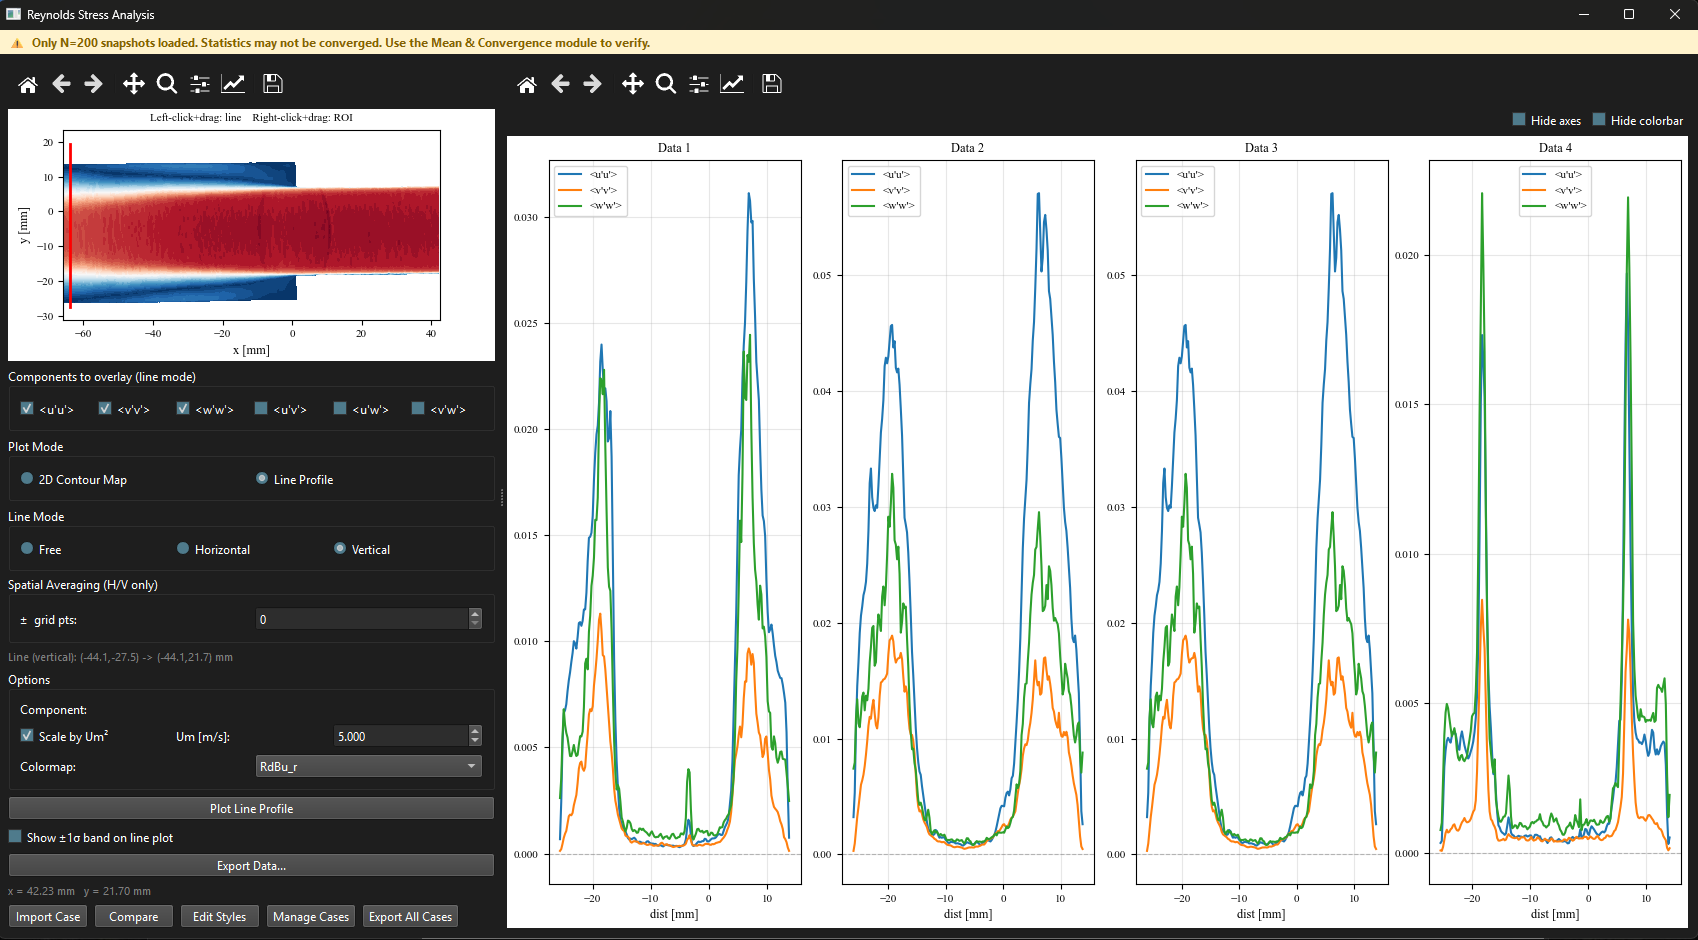
\includegraphics[width=0.92\linewidth]{fig_multicase_overlay}
  \caption{Reynolds stress line profile with two imported cases overlaid. The current dataset is shown as solid lines; imported cases use distinguishable colors and linestyles. The legend uses the user-assigned label per case.}
  \label{fig:multicase}
\end{figure}

\section{Managing cases}

Click \uipth{Manage Cases\ldots} to open the Case Manager dialog. From here, cases can be renamed, hidden, or removed. Each case retains its imported file path, line geometry (where applicable), and any header metadata such as $U_m$.

\begin{figure}[htbp]
  \centering
  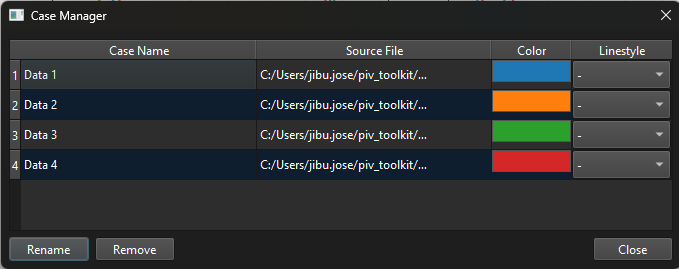
\includegraphics[width=0.55\linewidth]{fig_case_manager}
  \caption{Case Manager dialog. Each row corresponds to one imported case. Use the rename field to change the legend label; toggle visibility with the checkbox; click \uipth{Remove} to drop a case from the list.}
  \label{fig:casemgr}
\end{figure}

\section{Plot styles}

Click \uipth{Edit Styles\ldots} to change line color, linestyle, marker, and label per case. The current dataset and imported cases are styled independently.

\section{Quantity selector and layout chooser}

For modules with multiple quantities (Reynolds stresses with several components, TKE budget with $P$, $C$, $D$, $R$, etc.), the quantity selector controls which quantity is overlaid. The layout chooser switches between single-axes overlay and a faceted grid (one panel per case, sharing axes).

\section{Combined export}

Click \uipth{Export All Cases\ldots} to save the current dataset and all visible imported cases together in a single CSV. A \texttt{case} column is added to identify which row belongs to which case, suitable for pandas, MATLAB, or further plotting.

\section{Header consistency checks}

\software{uPrime} reads metadata from CSV headers when available. For Mean Velocity profiles, the \texttt{\# U\_m =} header is read per imported case. If the imported $U_m$ differs from the current setting, a status-bar warning is shown for that specific case so you can manually re-normalize before publishing.

\begin{warnbox}
\software{uPrime} does not automatically convert units between cases. If your imported CSV uses different units (mm vs m, m/s vs U/U\_m, etc.), the comparison will be misleading. Check the header values and re-export the source data in a consistent format if needed.
\end{warnbox}

% ============================= CHAPTER 14 ==============================
\chapter{Tips, Workflow, and Troubleshooting}

\section{Recommended workflow}

For any new dataset, follow this order:

\begin{enumerate}[leftmargin=1.5em]
  \item \textbf{Load} your files (\texttt{.dat} or \texttt{.mat}). Use stride subsampling if the dataset is large.
  \item \textbf{Set} acquisition type and $f_s$ in the popup dialog or the info ribbon.
  \item \textbf{Transform}: rotate to correct tilt, shift the origin to a physical reference.
  \item \textbf{Inspect} the mean field. Does the flow look correct? Right direction, sensible magnitudes?
  \item \textbf{Mean \& Convergence}: plot the mean velocity profile through your region of interest, then check at a representative point that first and second moments are converged. Skip $\langle u'u'u' \rangle$ if your dataset is small.
  \item \textbf{Reynolds stresses}: identify turbulent regions and shear layers.
  \item \textbf{TKE budget}: understand energy production and transport.
  \item \textbf{Correlations}: measure integral length and time scales.
  \item \textbf{POD}: identify dominant coherent structures.
  \item \textbf{DMD} (TR only): extract frequency-specific coherent modes.
  \item \textbf{Vortex identification}: locate and quantify vortex cores.
  \item \textbf{Export} results. Use the multi-case workflow to overlay against benchmark data when relevant.
\end{enumerate}

\section{Performance tips}

\begin{itemize}[leftmargin=1.5em]
  \item POD and DMD computation time scales as $N_t^2$. For 5000+ snapshots use stride subsampling to $\sim$1000--2000 samples first.
  \item Velocity data is loaded as 32-bit floats (float32), halving RAM usage compared to the 64-bit default.
  \item Close unused analysis windows to free RAM.
  \item Use \uipth{Reload Last Dataset} to undo a bad transform without restarting.
  \item For spatial spectra over a region, the FFT tab is faster than running multiple Welch lines.
  \item The $\Gamma_1/\Gamma_2$ computation involves a Python loop over all grid points and can be slow for large grids. Start with a subsampled dataset or a small neighborhood size $S$ while exploring.
  \item For very large \texttt{.mat} files, save with \texttt{-v7.3} in MATLAB to enable HDF5 chunked reading and real per-snapshot progress.
\end{itemize}

\section{Exporting figures for publication}

\begin{itemize}[leftmargin=1.5em]
  \item \textbf{PDF / SVG}: all text is embedded as editable text objects. Open in Adobe Illustrator or Inkscape to change fonts, sizes, and labels to match journal requirements.
  \item \textbf{PNG}: 300 DPI by default. Suitable for Word, PowerPoint, and reports.
  \item Enable \uipth{Clean export} and/or \uipth{Hide colorbar} for plain field images without annotations.
\end{itemize}

\section{Known limitations}

\begin{itemize}[leftmargin=1.5em]
  \item 3D (tomographic) PIV data is not supported.
  \item Pressure and viscous dissipation are not computed; the TKE budget residual absorbs these terms.
  \item Taylor hypothesis (for converting temporal to spatial scales) is only valid at low turbulence intensity ($u'/\langle U\rangle \ll 1$).
  \item Anisotropy analysis requires stereo data (2D3C) and will be unavailable for 2D2C datasets.
  \item DMD requires time-resolved data and a minimum of 50 snapshots.
  \item The $\Gamma_1/\Gamma_2$ computation is slower than gradient-based methods for large grids due to the neighborhood summation loop.
  \item All exported results are time-averaged unless otherwise noted. Per-snapshot export will be added in a future version.
  \item \texttt{.mat} files must contain multiple snapshots. Single-snapshot files are rejected before any data is loaded.
  \item For classic \texttt{.mat} files (not v7.3), the snapshot subset is applied after the full read because \texttt{scipy.io.loadmat} is a single blocking call. Convert to v7.3 in MATLAB for efficient strided loading on very large files.
\end{itemize}

\section{Common issues}

\begin{table}[htbp]
\centering
\caption{Common issues and solutions.}
\begin{tabular}{p{5.2cm}p{8.8cm}}
\toprule
\textbf{Issue} & \textbf{Solution} \\
\midrule
Files do not load (\texttt{.dat}) & Confirm files are Tecplot ASCII format from DaVis. Binary \texttt{.dat} files are not supported. \\
\addlinespace
\texttt{.mat} load shows ``Insufficient Snapshots'' immediately & The file contains only one snapshot. \software{uPrime} requires multiple snapshots. Re-export from MATLAB with the time axis included as the third dimension of \texttt{u}, \texttt{v}, etc. \\
\addlinespace
\texttt{.mat} variable dialog cannot find \texttt{u} & The velocity variable name is not in the recognized list. Use the manual dropdowns in the dialog to map your variables to $x$, $y$, $u$, $v$, etc. \\
\addlinespace
\texttt{.mat} dx/dy shown as 0.000 mm & Coordinate arrays are degenerate (all values equal along one axis), or the meshgrid orientation could not be inferred. Check that \texttt{x} and \texttt{y} contain real coordinate values. \\
\addlinespace
Anisotropy module is greyed out & Data is 2D2C. This module requires stereo (2D3C) data with a $W$ component. \\
\addlinespace
DMD button is greyed out & Set Acquisition Type to TR in the info ribbon and ensure at least 50 snapshots are loaded. \\
\addlinespace
Temporal tabs are greyed out & Set Acquisition Type to Time-Resolved and enter $f_s$ before opening the analysis window. \\
\addlinespace
Top-bar amber non-convergence label is shown & Dataset has fewer than 500 snapshots. Open Mean \& Convergence and verify convergence at a point in your region of interest. \\
\addlinespace
PDF save fails: permission denied & The file is open in Adobe Acrobat. Close it in Acrobat first, then save again. \\
\addlinespace
Rotation gives a blank result & Mirror the dataset \emph{before} rotating, not after. \\
\addlinespace
Lumley triangle points outside boundary & Insufficient snapshots or masked/invalid vectors near the sampling line. Avoid masked regions when drawing the analysis line. \\
\addlinespace
DMD spectrum dominated by high-$|\sigma|$ modes & Apply the growth rate filter ($|\sigma| <$ threshold) to focus on near-neutral physically meaningful modes. \\
\addlinespace
$\Gamma$ computation is very slow & Reduce the neighborhood half-width $S$, or subsample the dataset before computing. \\
\addlinespace
Imported case appears at wrong scale & The imported CSV uses a different $U_m$ or different units than the current session. Check the case's header and re-export consistently. \\
\bottomrule
\end{tabular}
\end{table}

% ============================= CHAPTER 15 ==============================
\chapter{Mouse and Keyboard Reference}

\section{Mouse interactions by window}

\begin{table}[htbp]
\centering
\caption{Mouse interactions in analysis windows.}
\begin{tabular}{lp{4cm}p{6.5cm}}
\toprule
\textbf{Window} & \textbf{Action} & \textbf{Effect} \\
\midrule
All windows       & Left-click on toolbar Home & Reset to original zoom \\
Main (Streamlines) & Left-click drag on field & Draw streamline seed rake \\
Mean \& Convergence (Tab 1) & Left-click drag on field & Draw line profile \\
Mean \& Convergence (Tab 2) & Left-click on field & Pick convergence point \\
Reynolds, TKE     & Left-click drag on field & Draw line profile \\
Spectra           & Left-click drag on field & Draw analysis line \\
Spectra           & Right-click drag on field & Draw rectangular ROI \\
Anisotropy        & Left-click drag on field & Draw Lumley triangle line \\
Anisotropy        & Left-click drag on field & Draw barycentric ROI (in Rectangle mode) \\
Correlation       & Left-click on field & Pick reference point (Point mode) \\
Correlation       & Left-click drag on field & Draw ROI (ROI mode) \\
Transform         & Left-click drag on preview & Draw rotation reference line \\
Transform         & Left-click on preview & Set new origin (Shift Origin mode) \\
DMD Spectrum      & Left-click on bubble & Select mode and show spatial structure \\
Vortex            & Left-click drag on field & Draw ROI (field view) \\
\bottomrule
\end{tabular}
\end{table}

\section{Keyboard shortcuts}

\begin{table}[htbp]
\centering
\caption{Keyboard shortcuts.}
\begin{tabular}{ll}
\toprule
\textbf{Key} & \textbf{Action} \\
\midrule
F1 & Open user manual \\
\bottomrule
\end{tabular}
\end{table}

\section{Field Viewer: Display Controls Summary}

\begin{table}[htbp]
\centering
\caption{Quick reference for display controls.}
\begin{tabular}{ll}
\toprule
\textbf{Control} & \textbf{Shortcut / location} \\
\midrule
Change displayed field     & \uipth{Field} dropdown in the options strip \\
Toggle overlay type        & \uipth{Overlay} radio buttons \\
Adjust vector density      & \uipth{Skip x} and \uipth{Skip y} spinboxes \\
Scale arrow/streamline length & \uipth{Length} spinbox \\
Scale arrowhead size       & \uipth{Arrow size} spinbox \\
Draw streamline rake       & Left-click drag on field (Streamlines overlay active) \\
Hide all axes and labels   & \uipth{Clean export} checkbox \\
Hide colorbar              & \uipth{Hide colorbar} checkbox \\
Reset view                 & \uipth{Home} button in toolbar \\
Save figure                & Save button in toolbar (PNG 300 DPI, PDF, SVG) \\
Open manual                & \uipth{? Manual} button (top right) or F1 \\
\bottomrule
\end{tabular}
\end{table}

% ============================= APPENDIX ================================
\appendix

\chapter{Citing uPrime}

If \software{uPrime} contributes to your research, please cite:

\begin{mdframed}[backgroundcolor=uplightgray, linecolor=upboxborder, linewidth=1pt]
Jibu Tom Jose, \& Ram, O. (2026). \textit{uPrime: Open-source software for velocity field and turbulence analysis from PIV and CFD data}. Transient Fluid Mechanics Laboratory (TFML), Technion (v0.6.0-alpha). Zenodo.\\
\url{https://doi.org/10.5281/zenodo.19376184}
\end{mdframed}

The citation text and DOI are also accessible directly from within the application via \uipth{About uPrime} at the bottom of the sidebar. The DOI can be copied to the clipboard using the copy button next to it.

\begin{figure}[htbp]
  \centering
  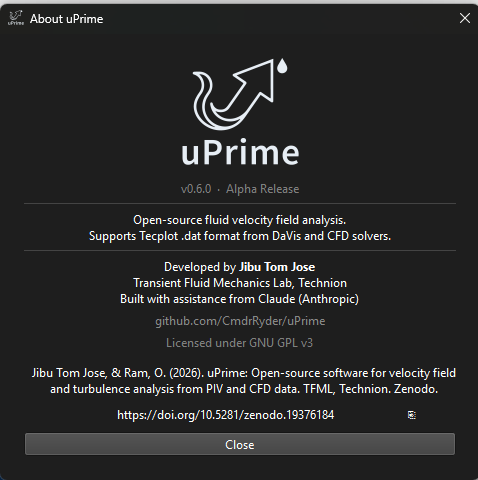
\includegraphics[width=0.5\linewidth]{fig_about}
  \caption{About \software{uPrime} dialog (v0.6.0). The citation text and DOI are displayed with a one-click copy button. The GitHub link opens the repository in the default browser.}
  \label{fig:about}
\end{figure}

\chapter{Sample Dataset}
\label{app:sample}

A sample dataset is available for testing and evaluating \software{uPrime} workflows without needing your own experimental data.

\begin{mdframed}[backgroundcolor=uplightgray, linecolor=upboxborder, linewidth=1pt]
\textbf{Download:} \url{https://doi.org/10.5281/zenodo.19539711}
\end{mdframed}

The dataset includes one non-time-resolved stereo PIV dataset (2D3C) with 100 snapshots, suitable for testing Reynolds stress, TKE budget, correlation, anisotropy, POD, and vortex identification modules; and one time-resolved planar PIV dataset (2D2C) with 200 snapshots, suitable for testing temporal spectra, temporal correlation, TR-POD, and DMD workflows.

Both datasets are provided in Tecplot ASCII \texttt{.dat} format and load directly into \software{uPrime} without any configuration.

\begin{warnbox}
This dataset is provided strictly for testing and evaluation of \software{uPrime}. It must not be used for research, publications, or redistribution without explicit written permission from the authors.
\end{warnbox}

\chapter{Version history}

\begin{longtable}{lp{12cm}}
\toprule
\textbf{Version} & \textbf{Summary} \\
\midrule
\endfirsthead

\multicolumn{2}{l}{\small\textit{(continued from previous page)}} \\
\toprule
\textbf{Version} & \textbf{Summary} \\
\midrule
\endhead

\midrule
\multicolumn{2}{r}{\small\textit{(continued on next page)}} \\
\endfoot

\bottomrule
\endlastfoot
v0.1   & Initial release: Reynolds stresses, TKE visualisation, basic spectral analysis. \\
v0.2   & TKE budget, anisotropy invariants, correlation analysis, coordinate transform. Migrated from PyQt5 to PyQt6. \\
v0.3   & POD analysis, improved correlation module (multiple scale methods, diagnostic plots), expanded transform tool. \\
v0.3.3 & Bug fixes (home button, mirror--rotate sequence, correlation ROI drawing). UI improvements: sidebar reorganized, dataset info ribbon, Times New Roman export font, 300\,DPI PNG. New features: snapshot subsampling and subset selection, reload button, mirror transform, exit confirmation dialog, hide axes/colorbar in all windows. \\
v0.3.4 & Streamline overlay: rake-based seed drawing, cumulative rakes, color picker, line width control. Spatial FFT tab: 2D ROI-based spatial spectra via pyFFTW. Memory halved: velocity arrays loaded as float32. Improved subset loading. Export improvements: 300\,DPI PNG, improved PDF quality. \\
v0.4.0 & New modules: DMD Analysis (TR only, frequency-growth rate spectrum, spatial mode viewer, Strouhal number support); Vortex Identification (vorticity, Q-criterion, $\lambda_{ci}$, $\lambda_2$, $\Gamma_1$/$\Gamma_2$, per-vortex statistics, spatial probability map). Non-destructive masking: raw velocity data never modified; mask stored as single 2D boolean array. Unit auto-detection from \texttt{.dat} file header. Acquisition type moved to dataset info ribbon with popup dialog on load. Correlation: 1/e method now returns interpolated crossing lag; zero-crossing marker placed at actual crossing position. Logo added to application and manual. User manual accessible via F1 or top-right button. \\
v0.4.1 & Performance: all heavy computations (POD, DMD, TKE budget, correlation, spectra, vortex identification) moved to background QThread workers; main window stays responsive during computation; progress indicator shown below compute button. Large dataset support: datasets exceeding 4\,GB are automatically memory-mapped to a temporary file in the system temp folder instead of being loaded into RAM; a warning with the temp path and required disk space is shown in the subsampling dialog. Bug fix: cursor value readout now reports correct values after mirror transform. \\
v0.5.0 & Multi-case comparison workflow added to Reynolds Stress, TKE Budget, Spectra, Correlation, and Anisotropy windows: Import Case, Edit Styles, Manage Cases, Combined CSV export. Export menu in main window with Tecplot ASCII mean field export. Term-visibility checkboxes (P/C/D/R) on TKE budget line plot. Reynolds stress $\pm 1\sigma$ band hidden by default. \\
v0.5.1 & New \uipth{Mean \& Convergence} module: first entry in the Analysis panel. Mean Velocity tab with line profiles, $U_m$ normalization, and multi-case import matching the Reynolds Stress workflow. Convergence tab with Welford online algorithm for cumulative first, second, and third central moments at a kernel-averaged picked point; sustained-crossing $N^*$ detection; grid layout (raw values) and single normalized layout. Convergence pop-up warnings removed and replaced by an inline amber top-bar label on Reynolds, TKE, and Spectra modules when $N < 500$. \\
v0.6.0 & MATLAB \texttt{.mat} file input (classic v5/v7 and v7.3 HDF5). Variable confirmation dialog with auto-detection, snapshot subset spinboxes, single-snapshot rejection. Auto-correction of meshgrid orientation and \texttt{(Nx, Ny, Nt)} velocity arrays. dx/dy estimated from coordinate arrays via robust median-of-differences. Default export filenames in Vortex Identification module. Mean \& Convergence picker fix for elongated fields (canvas height computed from data aspect). Field-display ZeroDivisionError guard. \\
\bottomrule
\end{longtable}

\end{document}